\documentclass{report}
\usepackage[margin=1in,marginparwidth=1.5in, marginparsep=.25in]{geometry}
\usepackage{fancyhdr}
\usepackage{amsmath}
\usepackage{amssymb}
\usepackage{tikz-qtree}
\usepackage{titlesec}
\usepackage{enumerate}
\usepackage{imakeidx}
\usepackage{multirow}
\usepackage[nonumberlist]{glossaries}
\usepackage[normalem]{ulem}
\usepackage{mathrsfs}
\usepackage{listings}
\usepackage{marvosym}
\usepackage{xcolor}
\usepackage{titlesec}
\usepackage{fontspec}
\usepackage{tcolorbox}
\usepackage{colortbl}
\usepackage{array}

\tcbuselibrary{skins}

\usetikzlibrary{arrows}

\def\l{\ensuremath{\lambda}}
\def\FV{\hbox{FV}}
\def\SN{\hbox{SN}}
\def\qed{\ensuremath{\square}}
\def\qqed{\ensuremath{\blacksquare}}
\def\rbeta{\ensuremath{\rightarrow_\beta}}
\def\concat{\ensuremath{\frown}}
\def\godnum#1{\ensuremath{\kern 0.02in\raisebox{.02in}{$\ulcorner$} \kern-.05in #1 \kern-.03in \raisebox{0.02in}{$\urcorner$}}}

\providecommand{\dotdiv}{% Don't redefine it if available
  \mathbin{% We want a binary operation
    \vphantom{+}% The same height as a plus or minus
    \text{% Change size in sub/superscripts
      \mathsurround=0pt % To be on the safe side
      \ooalign{% Superimpose the two symbols
        \noalign{\kern-.35ex}% but the dot is raised a bit
        \hidewidth$\smash{\cdot}$\hidewidth\cr % Dot
        \noalign{\kern.35ex}% Backup for vertical alignment
        $-$\cr % Minus
      }%
    }%
  }%
}

\def\monus{\dotdiv}
\def\v{\ensuremath{\mathcal{V}}}

% Margin Notes
\long\def\margnot#1#2{\marginpar{
    \begin{tikzpicture}
      \fill[color=txtbkblue] (0,-0.05) rectangle (5,0.55);
      \draw (0.2,0) node[anchor=south west] {\color{txtbkwhite}\textbf{#1}};
    \end{tikzpicture}#2
  }
}
\def\margnotTwo#1#2#3{\marginpar{
    \begin{tikzpicture}
      \fill[color=txtbkblue] (0,-0.45) rectangle (5,0.55);
      \draw (0.2,0) node[anchor=south west] {\color{txtbkwhite}\textbf{#1}};
      \draw (0.6,-.45) node[anchor=south west] {\color{txtbkwhite}\textbf{#2}};
    \end{tikzpicture}#3
  }
}

% Example Boxes
\long\def\examplebox#1#2{
  \begin{tcolorbox}[enhanced, width=\textwidth,colback={txtbkpaleblue},title={\color{txtbkwhite}\textbf{#1}},colupper=black,colbacktitle=txtbkblue,frame style={draw=none,fill=none}, arc=0pt,outer arc=0pt]
    #2
  \end{tcolorbox}
}
% Define macros and things to make the book look nice

% Colors
\definecolor{txtbkwhite}{RGB}{255,255,255}
\definecolor{txtbkblue}{RGB}{0,177,235}
\definecolor{txtbkpaleblue}{RGB}{224,242,253}
%\definecolor{txtbkblue}{RGB}{255,102,204}
%\definecolor{txtbkpaleblue}{RGB}{255,204,255}

\colorlet{coverblue}{txtbkblue!75!black}
\colorlet{coverpaleblue}{txtbkpaleblue!75!black}

% Remove fancyhdr line
\def\headrulewidth{0pt}

% Fonts
%\def\establishFont{\setmainfont{SourceSansPro-Regular}}
\def\establishFont{\setmainfont{Calibri}}
\newfontfamily\helvetica{DejaVuSans-ExtraLight}

% Sections and Subsections
\titleformat{\chapter}
            {\Huge\bfseries\color{txtbkwhite}\helvetica}
            {
              \begin{tikzpicture}[remember picture, overlay]
                \fill[color=txtbkblue] (current page.north west) rectangle (10,-1);
              \end{tikzpicture}
            }{0pt}{\huge}

\titleformat{\section}
            {\color{txtbkblue}\Large\bf}
            {
              \raisebox{-.1in}{
                \kern-1.2in
\begin{tikzpicture}
                \fill[color=txtbkblue] (0,0) rectangle (2.3,1);
                \draw (2.3,0.5) node[anchor=east] {\color{txtbkwhite}\thesection};
                \end{tikzpicture}\kern-0.15in
              }
            }{1em}{}

\titleformat{\subsection}
            {\color{txtbkblue}\bf\large}
            {\kern-.5in\large\thesubsection}{1em}{}

\def\plainFormat#1{} % Make it {#1} to enable.

%%%%%%%%%%%%%%%
% Set up page %
%%%%%%%%%%%%%%%
\lhead{\today}
\chead{21-366 Lambda Calculus Lecture Notes}
\rhead{Brian Jacobs}
\pagestyle{fancy}

\makeindex[options=-s Lambda-index.ist]
\makeglossaries
\setglossarystyle{altlist}
\newglossaryentry{term}
{
        name=Term,
        description={A term in \l calculus consists of constants and variables $x, y, z$ and other terms, $X, Y, Z$, arranged in one of the following ways. First, as a variable $x$. Second as $(XY)$, read ``$X$ applied to $Y$.'' Third, as a lambda term $(\l xX)$}
}

\newglossaryentry{program}
{
        name=Program,
        description={Any term in lambda calculus is referred to as a ``program.''}
}

\newglossaryentry{application}
{
        name=Application,
        description={An application of a term $X$ to another term $Y$ is written $XY$}
}

\newglossaryentry{redex}
{
        name=Redex,
        description={In a reduction, the redex is the initial term. It is replaced by the \textbf{reductum}}
}

\newglossaryentry{reductum}
{
        name=Reductum,
        description={In a reduction, the reductum is derived from the \textbf{redex}}
}

\newglossaryentry{combinator}
{
        name=Combinator,
        description={A term $X$ such that $FV(X) = \emptyset$. Alternately: a term which does not have any free variables. See \textbf{closed}}
}

\newglossaryentry{closed}
{
        name=Closed,
        description={A term $X$ such that $FV(X) = \emptyset$. Alternately: a term which does not have any free variables. See \textbf{combinator}}
}

\newglossaryentry{monussubtraction}
{
        name={Monus Subtraction},
        description={Notated $\dotdiv$, monus subtraction is defined as usual subtraction with the additional rule that if the subtraction results in a number lower than zero, it is defined to be $0$ instead}
}

\newglossaryentry{boolean}
{
        name={Boolean},
        description={A boolean can take one of two values, either true or false. We conventionally refer to true as $K := (\l xy.x)$ and false as $K_* := KI$}
}

\newglossaryentry{leftassociation}
{
        name={Left Association},
        description={When we delete every pair of parens around a subterm which is not in argument position, we can restore them by using left association (TODO: IMPROVE THIS)}
}

\newglossaryentry{ring}
{
        name={Ring},
        description={An algebraic structure comprised of a set and operations which generalize multiplication and addition to the elements of the set}
}

\newglossaryentry{diagonalize}
{
        name={Diagonalize},
        description={A function diagonalizes across its inputs by setting all of its inputs to be equal}
}

\newglossaryentry{fixedpoint}
{
        name={Fixed Point},
        description={A fixed point of a function is an element of the function's domain which is mapped to itself by that function. For example, if $f(x) = x$, then $x$ is a fixed point of $f$}
}

\newglossaryentry{tailrecursion}
{
        name={Tail Recursion},
        description={A tail recursive function is a function which calls itself at the end of its excecution}
}

\newglossaryentry{functionposition}
{
        name={Function Position},
        description={In a term $(UV)$, the $U$ is in function position}
}

\newglossaryentry{argumentposition}
{
        name={Argument Position},
        description={In a term $(UV)$, the $V$ is in function position}
}
\glsaddall

\title{21-366 Lambda Calculus \\\vspace{.2in} \normalsize Lecture Notes and Exercises}
\author{Brian Jacobs}
\date{\today}

\begin{document}
% Include Title Page
\pagestyle{empty}

\begin{tikzpicture}[remember picture,overlay]

  % Draw Background
  \fill[color=coverblue] (current page.south west) rectangle (current page.north east);
  \draw (current page.north west) node[anchor=north west] {
    \begin{minipage}{1.29\linewidth}
      \footnotesize\color{coverpaleblue} ( ( \l ( x ( \l ( x ( ( \l ( ( \l ( x ( ( \l ( x \l ) ) x ) ) ) \l ) ) ( x x ) ) ) ) ) ) ( ( \l ( ( \l ( x ( ( \l ( ( \l x ) x ) ) ( ( \l x ) x ) ) ) ) ( ( \l ( x ( ( \l ( x \l ) ) x ) ) ) ( ( \l ( x ( \l ( ( \l x ) x ) ) ) ) x ) ) ) ) ( x ( ( \l ( x ( ( \l ( ( \l ( x ( ( \l ( x \l ) ) x ) ) ) \l ) ) ( x x ) ) ) ) ( \l ( x ( ( \l ( x ( ( \l ( x \l ) ) x ) ) ) ( ( \l ( x \l ) ) x ) ) ) ) ) ) ) ) ( ( \l ( x ( \l ( x ( ( \l ( ( \l ( x ( ( \l ( x \l ) ) x ) ) ) \l ) ) ( x x ) ) ) ) ) ) ( ( \l ( ( \l ( x ( ( \l ( ( \l x ) x ) ) ( ( \l x ) x ) ) ) ) ( ( \l ( x ( ( \l ( x \l ) ) x ) ) ) ( ( \l ( x ( \l ( ( \l x ) x ) ) ) ) x ) ) ) ) ( x ( ( \l ( x ( ( \l ( ( \l ( x ( ( \l ( x \l ) ) x ) ) ) \l ) ) ( x x ) ) ) ) ( \l ( x ( ( \l ( x ( ( \l ( x \l ) ) x ) ) ) ( ( \l ( x \l ) ) x ) ) ) ) ) ) ) ) ( ( \l ( x ( \l ( x ( ( \l ( ( \l ( x ( ( \l ( x \l ) ) x ) ) ) \l ) ) ( x x ) ) ) ) ) ) ( ( \l ( ( \l ( x ( ( \l ( ( \l x ) x ) ) ( ( \l x ) x ) ) ) ) ( ( \l ( x ( ( \l ( x \l ) ) x ) ) ) ( ( \l ( x ( \l ( ( \l x ) x ) ) ) ) x ) ) ) ) ( x ( ( \l ( x ( ( \l ( ( \l ( x ( ( \l ( x \l ) ) x ) ) ) \l ) ) ( x x ) ) ) ) ( \l ( x ( ( \l ( x ( ( \l ( x \l ) ) x ) ) ) ( ( \l ( x \l ) ) x ) ) ) ) ) ) ) ) ( ( \l ( x ( \l ( x ( ( \l ( ( \l ( x ( ( \l ( x \l ) ) x ) ) ) \l ) ) ( x x ) ) ) ) ) ) ( ( \l ( ( \l ( x ( ( \l ( ( \l x ) x ) ) ( ( \l x ) x ) ) ) ) ( ( \l ( x ( ( \l ( x \l ) ) x ) ) ) ( ( \l ( x ( \l ( ( \l x ) x ) ) ) ) x ) ) ) ) ( x ( ( \l ( x ( ( \l ( ( \l ( x ( ( \l ( x \l ) ) x ) ) ) \l ) ) ( x x ) ) ) ) ( \l ( x ( ( \l ( x ( ( \l ( x \l ) ) x ) ) ) ( ( \l ( x \l ) ) x ) ) ) ) ) ) ) ) ( ( \l ( x ( \l ( x ( ( \l ( ( \l ( x ( ( \l ( x \l ) ) x ) ) ) \l ) ) ( x x ) ) ) ) ) ) ( ( \l ( ( \l ( x ( ( \l ( ( \l x ) x ) ) ( ( \l x ) x ) ) ) ) ( ( \l ( x ( ( \l ( x \l ) ) x ) ) ) ( ( \l ( x ( \l ( ( \l x ) x ) ) ) ) x ) ) ) ) ( x ( ( \l ( x ( ( \l ( ( \l ( x ( ( \l ( x \l ) ) x ) ) ) \l ) ) ( x x ) ) ) ) ( \l ( x ( ( \l ( x ( ( \l ( x \l ) ) x ) ) ) ( ( \l ( x \l ) ) x ) ) ) ) ) ) ) ) ( ( \l ( x ( \l ( x ( ( \l ( ( \l ( x ( ( \l ( x \l ) ) x ) ) ) \l ) ) ( x x ) ) ) ) ) ) ( ( \l ( ( \l ( x ( ( \l ( ( \l x ) x ) ) ( ( \l x ) x ) ) ) ) ( ( \l ( x ( ( \l ( x \l ) ) x ) ) ) ( ( \l ( x ( \l ( ( \l x ) x ) ) ) ) x ) ) ) ) ( x ( ( \l ( x ( ( \l ( ( \l ( x ( ( \l ( x \l ) ) x ) ) ) \l ) ) ( x x ) ) ) ) ( \l ( x ( ( \l ( x ( ( \l ( x \l ) ) x ) ) ) ( ( \l ( x \l ) ) x ) ) ) ) ) ) ) ) ( ( \l ( x ( \l ( x ( ( \l ( ( \l ( x ( ( \l ( x \l ) ) x ) ) ) \l ) ) ( x x ) ) ) ) ) ) ( ( \l ( ( \l ( x ( ( \l ( ( \l x ) x ) ) ( ( \l x ) x ) ) ) ) ( ( \l ( x ( ( \l ( x \l ) ) x ) ) ) ( ( \l ( x ( \l ( ( \l x ) x ) ) ) ) x ) ) ) ) ( x ( ( \l ( x ( ( \l ( ( \l ( x ( ( \l ( x \l ) ) x ) ) ) \l ) ) ( x x ) ) ) ) ( \l ( x ( ( \l ( x ( ( \l ( x \l ) ) x ) ) ) ( ( \l ( x \l ) ) x ) ) ) ) ) ) ) ) ( ( \l ( x ( \l ( x ( ( \l ( ( \l ( x ( ( \l ( x \l ) ) x ) ) ) \l ) ) ( x x ) ) ) ) ) ) ( ( \l ( ( \l ( x ( ( \l ( ( \l x ) x ) ) ( ( \l x ) x ) ) ) ) ( ( \l ( x ( ( \l ( x \l ) ) x ) ) ) ( ( \l ( x ( \l ( ( \l x ) x ) ) ) ) x ) ) ) ) ( x ( ( \l ( x ( ( \l ( ( \l ( x ( ( \l ( x \l ) ) x ) ) ) \l ) ) ( x x ) ) ) ) ( \l ( x ( ( \l ( x ( ( \l ( x \l ) ) x ) ) ) ( ( \l ( x \l ) ) x ) ) ) ) ) ) ) ) ( ( \l ( x ( \l ( x ( ( \l ( ( \l ( x ( ( \l ( x \l ) ) x ) ) ) \l ) ) ( x x ) ) ) ) ) ) ( ( \l ( ( \l ( x ( ( \l ( ( \l x ) x ) ) ( ( \l x ) x ) ) ) ) ( ( \l ( x ( ( \l ( x \l ) ) x ) ) ) ( ( \l ( x ( \l ( ( \l x ) x ) ) ) ) x ) ) ) ) ( x ( ( \l ( x ( ( \l ( ( \l ( x ( ( \l ( x \l ) ) x ) ) ) \l ) ) ( x x ) ) ) ) ( \l ( x ( ( \l ( x ( ( \l ( x \l ) ) x ) ) ) ( ( \l ( x \l ) ) x ) ) ) ) ) ) ) ) ( ( \l ( x ( \l ( x ( ( \l ( ( \l ( x ( ( \l ( x \l ) ) x ) ) ) \l ) ) ( x x ) ) ) ) ) ) ( ( \l ( ( \l ( x ( ( \l ( ( \l x ) x ) ) ( ( \l x ) x ) ) ) ) ( ( \l ( x ( ( \l ( x \l ) ) x ) ) ) ( ( \l ( x ( \l ( ( \l x ) x ) ) ) ) x ) ) ) ) ( x ( ( \l ( x ( ( \l ( ( \l ( x ( ( \l ( x \l ) ) x ) ) ) \l ) ) ( x x ) ) ) ) ( \l ( x ( ( \l ( x ( ( \l ( x \l ) ) x ) ) ) ( ( \l ( x \l ) ) x ) ) ) ) ) ) ) ) ( ( \l ( x ( \l ( x ( ( \l ( ( \l ( x ( ( \l ( x \l ) ) x ) ) ) \l ) ) ( x x ) ) ) ) ) ) ( ( \l ( ( \l ( x ( ( \l ( ( \l x ) x ) ) ( ( \l x ) x ) ) ) ) ( ( \l ( x ( ( \l ( x \l ) ) x ) ) ) ( ( \l ( x ( \l ( ( \l x ) x ) ) ) ) x ) ) ) ) ( x ( ( \l ( x ( ( \l ( ( \l ( x ( ( \l ( x \l ) ) x ) ) ) \l ) ) ( x x ) ) ) ) ( \l ( x ( ( \l ( x ( ( \l ( x \l ) ) x ) ) ) ( ( \l ( x \l ) ) x ) ) ) ) ) ) ) ) ( ( \l ( x ( \l ( x ( ( \l ( ( \l ( x ( ( \l ( x \l ) ) x ) ) ) \l ) ) ( x x ) ) ) ) ) ) ( ( \l ( ( \l ( x ( ( \l ( ( \l x ) x ) ) ( ( \l x ) x ) ) ) ) ( ( \l ( x ( ( \l ( x \l ) ) x ) ) ) ( ( \l ( x ( \l ( ( \l x ) x ) ) ) ) x ) ) ) ) ( x ( ( \l ( x ( ( \l ( ( \l ( x ( ( \l ( x \l ) ) x ) ) ) \l ) ) ( x x ) ) ) ) ( \l ( x ( ( \l ( x ( ( \l ( x \l ) ) x ) ) ) ( ( \l ( x \l ) ) x ) ) ) ) ) ) ) ) ( ( \l ( x ( \l ( x ( ( \l ( ( \l ( x ( ( \l ( x \l ) ) x ) ) ) \l ) ) ( x x ) ) ) ) ) ) ( ( \l ( ( \l ( x ( ( \l ( ( \l x ) x ) ) ( ( \l x ) x ) ) ) ) ( ( \l ( x ( ( \l ( x \l ) ) x ) ) ) ( ( \l ( x ( \l ( ( \l x ) x ) ) ) ) x ) ) ) ) ( x ( ( \l ( x ( ( \l ( ( \l ( x ( ( \l ( x \l ) ) x ) ) ) \l ) ) ( x x ) ) ) ) ( \l ( x ( ( \l ( x ( ( \l ( x \l ) ) x ) ) ) ( ( \l ( x \l ) ) x ) ) ) ) ) ) ) ) ( ( \l ( x ( \l ( x ( ( \l ( ( \l ( x ( ( \l ( x \l ) ) x ) ) ) \l ) ) ( x x ) ) ) ) ) ) ( ( \l ( ( \l ( x ( ( \l ( ( \l x ) x ) ) ( ( \l x ) x ) ) ) ) ( ( \l ( x ( ( \l ( x \l ) ) x ) ) ) ( ( \l ( x ( \l ( ( \l x ) x ) ) ) ) x ) ) ) ) ( x ( ( \l ( x ( ( \l ( ( \l ( x ( ( \l ( x \l ) ) x ) ) ) \l ) ) ( x x ) ) ) ) ( \l ( x ( ( \l ( x ( ( \l ( x \l ) ) x ) ) ) ( ( \l ( x \l ) ) x ) ) ) ) ) ) ) ) ( ( \l ( x ( \l ( x ( ( \l ( ( \l ( x ( ( \l ( x \l ) ) x ) ) ) \l ) ) ( x x ) ) ) ) ) ) ( ( \l ( ( \l ( x ( ( \l ( ( \l x ) x ) ) ( ( \l x ) x ) ) ) ) ( ( \l ( x ( ( \l ( x \l ) ) x ) ) ) ( ( \l ( x ( \l ( ( \l x ) x ) ) ) ) x ) ) ) ) ( x ( ( \l ( x ( ( \l ( ( \l ( x ( ( \l ( x \l ) ) x ) ) ) \l ) ) ( x x ) ) ) ) ( \l ( x ( ( \l ( x ( ( \l ( x \l ) ) x ) ) ) ( ( \l ( x \l ) ) x ) ) ) ) ) ) ) ) ( ( \l ( x ( \l ( x ( ( \l ( ( \l ( x ( ( \l ( x \l ) ) x ) ) ) \l ) ) ( x x ) ) ) ) ) ) ( ( \l ( ( \l ( x ( ( \l ( ( \l x ) x ) ) ( ( \l x ) x ) ) ) ) ( ( \l ( x ( ( \l ( x \l ) ) x ) ) ) ( ( \l ( x ( \l ( ( \l x ) x ) ) ) ) x ) ) ) ) ( x ( ( \l ( x ( ( \l ( ( \l ( x ( ( \l ( x \l ) ) x ) ) ) \l ) ) ( x x ) ) ) ) ( \l ( x ( ( \l ( x ( ( \l ( x \l ) ) x ) ) ) ( ( \l ( x \l ) ) x ) ) ) ) ) ) ) ) ( ( \l ( x ( \l ( x ( ( \l ( ( \l ( x ( ( \l ( x \l ) ) x ) ) ) \l ) ) ( x x ) ) ) ) ) ) ( ( \l ( ( \l ( x ( ( \l ( ( \l x ) x ) ) ( ( \l x ) x ) ) ) ) ( ( \l ( x ( ( \l ( x \l ) ) x ) ) ) ( ( \l ( x ( \l ( ( \l x ) x ) ) ) ) x ) ) ) ) ( x ( ( \l ( x ( ( \l ( ( \l ( x ( ( \l ( x \l ) ) x ) ) ) \l ) ) ( x x ) ) ) ) ( \l ( x ( ( \l ( x ( ( \l ( x \l ) ) x ) ) ) ( ( \l ( x \l ) ) x ) ) ) ) ) ) ) ) ( ( \l ( x ( \l ( x ( ( \l ( ( \l ( x ( ( \l ( x \l ) ) x ) ) ) \l ) ) ( x x ) ) ) ) ) ) ( ( \l ( ( \l ( x ( ( \l ( ( \l x ) x ) ) ( ( \l x ) x ) ) ) ) ( ( \l ( x ( ( \l ( x \l ) ) x ) ) ) ( ( \l ( x ( \l ( ( \l x ) x ) ) ) ) x ) ) ) ) ( x ( ( \l ( x ( ( \l ( ( \l ( x ( ( \l ( x \l ) ) x ) ) ) \l ) ) ( x x ) ) ) ) ( \l ( x ( ( \l ( x ( ( \l ( x \l ) ) x ) ) ) ( ( \l ( x \l ) ) x ) ) ) ) ) ) ) ) ( ( \l ( x ( \l ( x ( ( \l ( ( \l ( x ( ( \l ( x \l ) ) x ) ) ) \l ) ) ( x x ) ) ) ) ) ) ( ( \l ( ( \l ( x ( ( \l ( ( \l x ) x ) ) ( ( \l x ) x ) ) ) ) ( ( \l ( x ( ( \l ( x \l ) ) x ) ) ) ( ( \l ( x ( \l ( ( \l x ) x ) ) ) ) x ) ) ) ) ( x ( ( \l ( x ( ( \l ( ( \l ( x ( ( \l ( x \l ) ) x ) ) ) \l ) ) ( x x ) ) ) ) ( \l ( x ( ( \l ( x ( ( \l ( x \l ) ) x ) ) ) ( ( \l ( x \l ) ) x ) ) ) ) ) ) ) ) ( ( \l ( x ( \l ( x ( ( \l ( ( \l ( x ( ( \l ( x \l ) ) x ) ) ) \l ) ) ( x x ) ) ) ) ) ) ( ( \l ( ( \l ( x ( ( \l ( ( \l x ) x ) ) ( ( \l x ) x ) ) ) ) ( ( \l ( x ( ( \l ( x \l ) ) x ) ) ) ( ( \l ( x ( \l ( ( \l x ) x ) ) ) ) x ) ) ) ) ( x ( ( \l ( x ( ( \l ( ( \l ( x ( ( \l ( x \l ) ) x ) ) ) \l ) ) ( x x ) ) ) ) ( \l ( x ( ( \l ( x ( ( \l ( x \l ) ) x ) ) ) ( ( \l ( x \l ) ) x ) ) ) ) ) ) ) ) ( ( \l ( x ( \l ( x ( ( \l ( ( \l ( x ( ( \l ( x \l ) ) x ) ) ) \l ) ) ( x x ) ) ) ) ) ) ( ( \l ( ( \l ( x ( ( \l ( ( \l x ) x ) ) ( ( \l x ) x ) ) ) ) ( ( \l ( x ( ( \l ( x \l ) ) x ) ) ) ( ( \l ( x ( \l ( ( \l x ) x ) ) ) ) x ) ) ) ) ( x ( ( \l ( x ( ( \l ( ( \l ( x ( ( \l ( x \l ) ) x ) ) ) \l ) ) ( x x ) ) ) ) ( \l ( x ( ( \l ( x ( ( \l ( x \l ) ) x ) ) ) ( ( \l ( x \l ) ) x ) ) ) ) ) ) ) ) ( ( \l ( x ( \l ( x ( ( \l ( ( \l ( x ( ( \l ( x \l ) ) x ) ) ) \l ) ) ( x x ) ) ) ) ) ) ( ( \l ( ( \l ( x ( ( \l ( ( \l x ) x ) ) ( ( \l x ) x ) ) ) ) ( ( \l ( x ( ( \l ( x \l ) ) x ) ) ) ( ( \l ( x ( \l ( ( \l x ) x ) ) ) ) x ) ) ) ) ( x ( ( \l ( x ( ( \l ( ( \l ( x ( ( \l ( x \l ) ) x ) ) ) \l ) ) ( x x ) ) ) ) ( \l ( x ( ( \l ( x ( ( \l ( x \l ) ) x ) ) ) ( ( \l ( x \l ) ) x ) ) ) ) ) ) ) ) ( ( \l ( x ( \l ( x ( ( \l ( ( \l ( x ( ( \l ( x \l ) ) x ) ) ) \l ) ) ( x x ) ) ) ) ) ) ( ( \l ( ( \l ( x ( ( \l ( ( \l x ) x ) ) ( ( \l x ) x ) ) ) ) ( ( \l ( x ( ( \l ( x \l ) ) x ) ) ) ( ( \l ( x ( \l ( ( \l x ) x ) ) ) ) x ) ) ) ) ( x ( ( \l ( x ( ( \l ( ( \l ( x ( ( \l ( x \l ) ) x ) ) ) \l ) ) ( x x ) ) ) ) ( \l ( x ( ( \l ( x ( ( \l ( x \l ) ) x ) ) ) ( ( \l ( x \l ) ) x ) ) ) ) ) ) ) ) ( ( \l ( x ( \l ( x ( ( \l ( ( \l ( x ( ( \l ( x \l ) ) x ) ) ) \l ) ) ( x x ) ) ) ) ) ) ( ( \l ( ( \l ( x ( ( \l ( ( \l x ) x ) ) ( ( \l x ) x ) ) ) ) ( ( \l ( x ( ( \l ( x \l ) ) x ) ) ) ( ( \l ( x ( \l ( ( \l x ) x ) ) ) ) x ) ) ) ) ( x ( ( \l ( x ( ( \l ( ( \l ( x ( ( \l ( x \l ) ) x ) ) ) \l ) ) ( x x ) ) ) ) ( \l ( x ( ( \l ( x ( ( \l ( x \l ) ) x ) ) ) ( ( \l ( x \l ) ) x ) ) ) ) ) ) ) ) ( ( \l ( x ( \l ( x ( ( \l ( ( \l ( x ( ( \l ( x \l ) ) x ) ) ) \l ) ) ( x x ) ) ) ) ) ) ( ( \l ( ( \l ( x ( ( \l ( ( \l x ) x ) ) ( ( \l x ) x ) ) ) ) ( ( \l ( x ( ( \l ( x \l ) ) x ) ) ) ( ( \l ( x ( \l ( ( \l x ) x ) ) ) ) x ) ) ) ) ( x ( ( \l ( x ( ( \l ( ( \l ( x ( ( \l ( x \l ) ) x ) ) ) \l ) ) ( x x ) ) ) ) ( \l ( x ( ( \l ( x ( ( \l ( x \l ) ) x ) ) ) ( ( \l ( x \l ) ) x ) ) ) ) ) ) ) ) ( ( \l ( x ( \l ( x ( ( \l ( ( \l ( x ( ( \l ( x \l ) ) x ) ) ) \l ) ) ( x x ) ) ) ) ) ) ( ( \l ( ( \l ( x ( ( \l ( ( \l x ) x ) ) ( ( \l x ) x ) ) ) ) ( ( \l ( x ( ( \l ( x \l ) ) x ) ) ) ( ( \l ( x ( \l ( ( \l x ) x ) ) ) ) x ) ) ) ) ( x ( ( \l ( x ( ( \l ( ( \l ( x ( ( \l ( x \l ) ) x ) ) ) \l ) ) ( x x ) ) ) ) ( \l ( x ( ( \l ( x ( ( \l ( x \l ) ) x ) ) ) ( ( \l ( x \l ) ) x ) ) ) ) ) ) ) ) ( ( \l ( x ( \l ( x ( ( \l ( ( \l ( x ( ( \l ( x \l ) ) x ) ) ) \l ) ) ( x x ) ) ) ) ) ) ( ( \l ( ( \l ( x ( ( \l ( ( \l x ) x ) ) ( ( \l x ) x ) ) ) ) ( ( \l ( x ( ( \l ( x \l ) ) x ) ) ) ( ( \l ( x ( \l ( ( \l x ) x ) ) ) ) x ) ) ) ) ( x ( ( \l ( x ( ( \l ( ( \l ( x ( ( \l ( x \l ) ) x ) ) ) \l ) ) ( x x ) ) ) ) ( \l ( x ( ( \l ( x ( ( \l ( x \l ) ) x ) ) ) ( ( \l ( x \l ) ) x ) ) ) ) ) ) ) ) ( ( \l ( x ( \l ( x ( ( \l ( ( \l ( x ( ( \l ( x \l ) ) x ) ) ) \l ) ) ( x x ) ) ) ) ) ) ( ( \l ( ( \l ( x ( ( \l ( ( \l x ) x ) ) ( ( \l x ) x ) ) ) ) ( ( \l ( x ( ( \l ( x \l ) ) x ) ) ) ( ( \l ( x ( \l ( ( \l x ) x ) ) ) ) x ) ) ) ) ( x ( ( \l ( x ( ( \l ( ( \l ( x ( ( \l ( x \l ) ) x ) ) ) \l ) ) ( x x ) ) ) ) ( \l ( x ( ( \l ( x ( ( \l ( x \l ) ) x ) ) ) ( ( \l ( x \l ) ) x ) ) ) ) ) ) ) ) ( ( \l ( x ( \l ( x ( ( \l ( ( \l ( x ( ( \l ( x \l ) ) x ) ) ) \l ) ) ( x x ) ) ) ) ) ) ( ( \l ( ( \l ( x ( ( \l ( ( \l x ) x ) ) ( ( \l x ) x ) ) ) ) ( ( \l ( x ( ( \l ( x \l ) ) x ) ) ) ( ( \l ( x ( \l ( ( \l x ) x ) ) ) ) x ) ) ) ) ( x ( ( \l ( x ( ( \l ( ( \l ( x ( ( \l ( x \l ) ) x ) ) ) \l ) ) ( x x ) ) ) ) ( \l ( x ( ( \l ( x ( ( \l ( x \l ) ) x ) ) ) ( ( \l ( x \l ) ) x ) ) ) ) ) ) ) ) ( ( \l ( x ( \l ( x ( ( \l ( ( \l ( x ( ( \l ( x \l ) ) x ) ) ) \l ) ) ( x x ) ) ) ) ) ) ( ( \l ( ( \l ( x ( ( \l ( ( \l x ) x ) ) ( ( \l x ) x ) ) ) ) ( ( \l ( x ( ( \l ( x \l ) ) x ) ) ) ( ( \l ( x ( \l ( ( \l x ) x ) ) ) ) x ) ) ) ) ( x ( ( \l ( x ( ( \l ( ( \l ( x ( ( \l ( x \l ) ) x ) ) ) \l ) ) ( x x ) ) ) ) ( \l ( x ( ( \l ( x ( ( \l ( x \l ) ) x ) ) ) ( ( \l ( x \l ) ) x ) ) ) ) ) ) ) ) ( ( \l ( x ( \l ( x ( ( \l ( ( \l ( x ( ( \l ( x \l ) ) x ) ) ) \l ) ) ( x x ) ) ) ) ) ) ( ( \l ( ( \l ( x ( ( \l ( ( \l x ) x ) ) ( ( \l x ) x ) ) ) ) ( ( \l ( x ( ( \l ( x \l ) ) x ) ) ) ( ( \l ( x ( \l ( ( \l x ) x ) ) ) ) x ) ) ) ) ( x ( ( \l ( x ( ( \l ( ( \l ( x ( ( \l ( x \l ) ) x ) ) ) \l ) ) ( x x ) ) ) ) ( \l ( x ( ( \l ( x ( ( \l ( x \l ) ) x ) ) ) ( ( \l ( x \l ) ) x ) ) ) ) ) ) ) ) ( ( \l ( x ( \l ( x ( ( \l ( ( \l ( x ( ( \l ( x \l ) ) x ) ) ) \l ) ) ( x x ) ) ) ) ) ) ( ( \l ( ( \l ( x ( ( \l ( ( \l x ) x ) ) ( ( \l x ) x ) ) ) ) ( ( \l ( x ( ( \l ( x \l ) ) x ) ) ) ( ( \l ( x ( \l ( ( \l x ) x ) ) ) ) x ) ) ) ) ( x ( ( \l ( x ( ( \l ( ( \l ( x ( ( \l ( x \l ) ) x ) ) ) \l ) ) ( x x ) ) ) ) ( \l ( x ( ( \l ( x ( ( \l ( x \l ) ) x ) ) ) ( ( \l ( x \l ) ) x ) ) ) ) ) ) ) ) ( ( \l ( x ( \l ( x ( ( \l ( ( \l ( x ( ( \l ( x \l ) ) x ) ) ) \l ) ) ( x x ) ) ) ) ) ) ( ( \l ( ( \l ( x ( ( \l ( ( \l x ) x ) ) ( ( \l x ) x ) ) ) ) ( ( \l ( x ( ( \l ( x \l ) ) x ) ) ) ( ( \l ( x ( \l ( ( \l x ) x ) ) ) ) x ) ) ) ) ( x ( ( \l ( x ( ( \l ( ( \l ( x ( ( \l ( x \l ) ) x ) ) ) \l ) ) ( x x ) ) ) ) ( \l ( x ( ( \l ( x ( ( \l ( x \l ) ) x ) ) ) ( ( \l ( x \l ) ) x ) ) ) ) ) ) ) ) ( ( \l ( x ( \l ( x ( ( \l ( ( \l ( x ( ( \l ( x \l ) ) x ) ) ) \l ) ) ( x x ) ) ) ) ) ) ( ( \l ( ( \l ( x ( ( \l ( ( \l x ) x ) ) ( ( \l x ) x ) ) ) ) ( ( \l ( x ( ( \l ( x \l ) ) x ) ) ) ( ( \l ( x ( \l ( ( \l x ) x ) ) ) ) x ) ) ) ) ( x ( ( \l ( x ( ( \l ( ( \l ( x ( ( \l ( x \l ) ) x ) ) ) \l ) ) ( x x ) ) ) ) ( \l ( x ( ( \l ( x ( ( \l ( x \l ) ) x ) ) ) ( ( \l ( x \l ) ) x ) ) ) ) ) ) ) ) ( ( \l ( x ( \l ( x ( ( \l ( ( \l ( x ( ( \l ( x \l ) ) x ) ) ) \l ) ) ( x x ) ) ) ) ) ) ( ( \l ( ( \l ( x ( ( \l ( ( \l x ) x ) ) ( ( \l x ) x ) ) ) ) ( ( \l ( x ( ( \l ( x \l ) ) x ) ) ) ( ( \l ( x ( \l ( ( \l x ) x ) ) ) ) x ) ) ) ) ( x ( ( \l ( x ( ( \l ( ( \l ( x ( ( \l ( x \l ) ) x ) ) ) \l ) ) ( x x ) ) ) ) ( \l ( x ( ( \l ( x ( ( \l ( x \l ) ) x ) ) ) ( ( \l ( x \l ) ) x ) ) ) ) ) ) ) ) ( ( \l ( x ( \l ( x ( ( \l ( ( \l ( x ( ( \l ( x \l ) ) x ) ) ) \l ) ) ( x x ) ) ) ) ) ) ( ( \l ( ( \l ( x ( ( \l ( ( \l x ) x ) ) ( ( \l x ) x ) ) ) ) ( ( \l ( x ( ( \l ( x \l ) ) x ) ) ) ( ( \l ( x ( \l ( ( \l x ) x ) ) ) ) x ) ) ) ) ( x ( ( \l ( x ( ( \l ( ( \l ( x ( ( \l ( x \l ) ) x ) ) ) \l ) ) ( x x ) ) ) ) ( \l ( x ( ( \l ( x ( ( \l ( x \l ) ) x ) ) ) ( ( \l ( x \l ) ) x ) ) ) ) ) ) ) ) ( ( \l ( x ( \l ( x ( ( \l ( ( \l ( x ( ( \l ( x \l ) ) x ) ) ) \l ) ) ( x x ) ) ) ) ) ) ( ( \l ( ( \l ( x ( ( \l ( ( \l x ) x ) ) ( ( \l x ) x ) ) ) ) ( ( \l ( x ( ( \l ( x \l ) ) x ) ) ) ( ( \l ( x ( \l ( ( \l x ) x ) ) ) ) x ) ) ) ) ( x ( ( \l ( x ( ( \l ( ( \l ( x ( ( \l ( x \l ) ) x ) ) ) \l ) ) ( x x ) ) ) ) ( \l ( x ( ( \l ( x ( ( \l ( x \l ) ) x ) ) ) ( ( \l ( x \l ) ) x ) ) ) ) ) ) ) ) ( ( \l ( x ( \l ( x ( ( \l ( ( \l ( x ( ( \l ( x \l ) ) x ) ) ) \l ) ) ( x x ) ) ) ) ) ) ( ( \l ( ( \l ( x ( ( \l ( ( \l x ) x ) ) ( ( \l x ) x ) ) ) ) ( ( \l ( x ( ( \l ( x \l ) ) x ) ) ) ( ( \l ( x ( \l ( ( \l x ) x ) ) ) ) x ) ) ) ) ( x ( ( \l ( x ( ( \l ( ( \l ( x ( ( \l ( x \l ) ) x ) ) ) \l ) ) ( x x ) ) ) ) ( \l ( x ( ( \l ( x ( ( \l ( x \l ) ) x ) ) ) ( ( \l ( x \l ) ) x ) ) ) ) ) ) ) ) ( ( \l ( x ( \l ( x ( ( \l ( ( \l ( x ( ( \l ( x \l ) ) x ) ) ) \l ) ) ( x x ) ) ) ) ) ) ( ( \l ( ( \l ( x ( ( \l ( ( \l x ) x ) ) ( ( \l x ) x ) ) ) ) ( ( \l ( x ( ( \l ( x \l ) ) x ) ) ) ( ( \l ( x ( \l ( ( \l x ) x ) ) ) ) x ) ) ) ) ( x ( ( \l ( x ( ( \l ( ( \l ( x ( ( \l ( x \l ) ) x ) ) ) \l ) ) ( x x ) ) ) ) ( \l ( x ( ( \l ( x ( ( \l ( x \l ) ) x ) ) ) ( ( \l ( x \l ) ) x ) ) ) ) ) ) ) ) ( ( \l ( x ( \l ( x ( ( \l ( ( \l ( x ( ( \l ( x \l ) ) x ) ) ) \l ) ) ( x x ) ) ) ) ) ) ( ( \l ( ( \l ( x ( ( \l ( ( \l x ) x ) ) ( ( \l x ) x ) ) ) ) ( ( \l ( x ( ( \l ( x \l ) ) x ) ) ) ( ( \l ( x ( \l ( ( \l x ) x ) ) ) ) x ) ) ) ) ( x ( ( \l ( x ( ( \l ( ( \l ( x ( ( \l ( x \l ) ) x ) ) ) \l ) ) ( x x ) ) ) ) ( \l ( x ( ( \l ( x ( ( \l ( x \l ) ) x ) ) ) ( ( \l ( x \l ) ) x ) ) ) ) ) ) ) ) ( ( \l ( x ( \l ( x ( ( \l ( ( \l ( x ( ( \l ( x \l ) ) x ) ) ) \l ) ) ( x x ) ) ) ) ) ) ( ( \l ( ( \l ( x ( ( \l ( ( \l x ) x ) ) ( ( \l x ) x ) ) ) ) ( ( \l ( x ( ( \l ( x \l ) ) x ) ) ) ( ( \l ( x ( \l ( ( \l x ) x ) ) ) ) x ) ) ) ) ( x ( ( \l ( x ( ( \l ( ( \l ( x ( ( \l ( x \l ) ) x ) ) ) \l ) ) ( x x ) ) ) ) ( \l ( x ( ( \l ( x ( ( \l ( x \l ) ) x ) ) ) ( ( \l ( x \l ) ) x ) ) ) ) ) ) ) ) ( ( \l ( x ( \l ( x ( ( \l ( ( \l ( x ( ( \l ( x \l ) ) x ) ) ) \l ) ) ( x x ) ) ) ) ) ) ( ( \l ( ( \l ( x ( ( \l ( ( \l x ) x ) ) ( ( \l x ) x ) ) ) ) ( ( \l ( x ( ( \l ( x \l ) ) x ) ) ) ( ( \l ( x ( \l ( ( \l x ) x ) ) ) ) x ) ) ) ) ( x ( ( \l ( x ( ( \l ( ( \l ( x ( ( \l ( x \l ) ) x ) ) ) \l ) ) ( x x ) ) ) ) ( \l ( x ( ( \l ( x ( ( \l ( x \l ) ) x ) ) ) ( ( \l ( x \l ) ) x ) ) ) ) ) ) ) ) ( ( \l ( x ( \l ( x ( ( \l ( ( \l ( x ( ( \l ( x \l ) ) x ) ) ) \l ) ) ( x x ) ) ) ) ) ) ( ( \l ( ( \l ( x ( ( \l ( ( \l x ) x ) ) ( ( \l x ) x ) ) ) ) ( ( \l ( x ( ( \l ( x \l ) ) x ) ) ) ( ( \l ( x ( \l ( ( \l x ) x ) ) ) ) x ) ) ) ) ( x ( ( \l ( x ( ( \l ( ( \l ( x ( ( \l ( x \l ) ) x ) ) ) \l ) ) ( x x ) ) ) ) ( \l ( x ( ( \l ( x ( ( \l ( x \l ) ) x ) ) ) ( ( \l ( x \l ) ) x ) ) ) ) ) ) ) ) ( ( \l ( x ( \l ( x ( ( \l ( ( \l ( x ( ( \l ( x \l ) ) x ) ) ) \l ) ) ( x x ) ) ) ) ) ) ( ( \l ( ( \l ( x ( ( \l ( ( \l x ) x ) ) ( ( \l x ) x ) ) ) ) ( ( \l ( x ( ( \l ( x \l ) ) x ) ) ) ( ( \l ( x ( \l ( ( \l x ) x ) ) ) ) x ) ) ) ) ( x ( ( \l ( x ( ( \l ( ( \l ( x ( ( \l ( x \l ) ) x ) ) ) \l ) ) ( x x ) ) ) ) ( \l ( x ( ( \l ( x ( ( \l ( x \l ) ) x ) ) ) ( ( \l ( x \l ) ) x ) ) ) ) ) ) ) ) ( ( \l ( x ( \l ( x ( ( \l ( ( \l ( x ( ( \l ( x \l ) ) x ) ) ) \l ) ) ( x x ) ) ) ) ) ) ( ( \l ( ( \l ( x ( ( \l ( ( \l x ) x ) ) ( ( \l x ) x ) ) ) ) ( ( \l ( x ( ( \l ( x \l ) ) x ) ) ) ( ( \l ( x ( \l ( ( \l x ) x ) ) ) ) x ) ) ) ) ( x ( ( \l ( x ( ( \l ( ( \l ( x ( ( \l ( x \l ) ) x ) ) ) \l ) ) ( x x ) ) ) ) ( \l ( x ( ( \l ( x ( ( \l ( x \l ) ) x ) ) ) ( ( \l ( x \l ) ) x ) ) ) ) ) ) ) ) ( ( \l ( x ( \l ( x ( ( \l ( ( \l ( x ( ( \l ( x \l ) ) x ) ) ) \l ) ) ( x x ) ) ) ) ) ) ( ( \l ( ( \l ( x ( ( \l ( ( \l x ) x ) ) ( ( \l x ) x ) ) ) ) ( ( \l ( x ( ( \l ( x \l ) ) x ) ) ) ( ( \l ( x ( \l ( ( \l x ) x ) ) ) ) x ) ) ) ) ( x ( ( \l ( x ( ( \l ( ( \l ( x ( ( \l ( x \l ) ) x ) ) ) \l ) ) ( x x ) ) ) ) ( \l ( x ( ( \l ( x ( ( \l ( x \l ) ) x ) ) ) ( ( \l ( x \l ) ) x ) ) ) ) ) ) ) ) ( ( \l ( x ( \l ( x ( ( \l ( ( \l ( x ( ( \l ( x \l ) ) x ) ) ) \l ) ) ( x x ) ) ) ) ) ) ( ( \l ( ( \l ( x ( ( \l ( ( \l x ) x ) ) ( ( \l x ) x ) ) ) ) ( ( \l ( x ( ( \l ( x \l ) ) x ) ) ) ( ( \l ( x ( \l ( ( \l x ) x ) ) ) ) x ) ) ) ) ( x ( ( \l ( x ( ( \l ( ( \l ( x ( ( \l ( x \l ) ) x ) ) ) \l ) ) ( x x ) ) ) ) ( \l ( x ( ( \l ( x ( ( \l ( x \l ) ) x ) ) ) ( ( \l ( x \l ) ) x ) ) ) ) ) ) ) ) ( ( \l ( x ( \l ( x ( ( \l ( ( \l ( x ( ( \l ( x \l ) ) x ) ) ) \l ) ) ( x x ) ) ) ) ) ) ( ( \l ( ( \l ( x ( ( \l ( ( \l x ) x ) ) ( ( \l x ) x ) ) ) ) ( ( \l ( x ( ( \l ( x \l ) ) x ) ) ) ( ( \l ( x ( \l ( ( \l x ) x ) ) ) ) x ) ) ) ) ( x ( ( \l ( x ( ( \l ( ( \l ( x ( ( \l ( x \l ) ) x ) ) ) \l ) ) ( x x ) ) ) ) ( \l ( x ( ( \l ( x ( ( \l ( x \l ) ) x ) ) ) ( ( \l ( x \l ) ) x ) ) ) ) ) ) ) ) ( ( \l ( x ( \l ( x ( ( \l ( ( \l ( x ( ( \l ( x \l ) ) x ) ) ) \l ) ) ( x x ) ) ) ) ) ) ( ( \l ( ( \l ( x ( ( \l ( ( \l x ) x ) ) ( ( \l x ) x ) ) ) ) ( ( \l ( x ( ( \l ( x \l ) ) x ) ) ) ( ( \l ( x ( \l ( ( \l x ) x ) ) ) ) x ) ) ) ) ( x ( ( \l ( x ( ( \l ( ( \l ( x ( ( \l ( x \l ) ) x ) ) ) \l ) ) ( x x ) ) ) ) ( \l ( x ( ( \l ( x ( ( \l ( x \l ) ) x ) ) ) ( ( \l ( x \l ) ) x ) ) ) ) ) ) ) ) ( ( \l ( x ( \l ( x ( ( \l ( ( \l ( x ( ( \l ( x \l ) ) x ) ) ) \l ) ) ( x x ) ) ) ) ) ) ( ( \l ( ( \l ( x ( ( \l ( ( \l x ) x ) ) ( ( \l x ) x ) ) ) ) ( ( \l ( x ( ( \l ( x \l ) ) x ) ) ) ( ( \l ( x ( \l ( ( \l x ) x ) ) ) ) x ) ) ) ) ( x ( ( \l ( x ( ( \l ( ( \l ( x ( ( \l ( x \l ) ) x ) ) ) \l ) ) ( x x ) ) ) ) ( \l ( x ( ( \l ( x ( ( \l ( x \l ) ) x ) ) ) ( ( \l ( x \l ) ) x ) ) ) ) ) ) ) ) ( ( \l ( x ( \l ( x ( ( \l ( ( \l ( x ( ( \l ( x \l ) ) x ) ) ) \l ) ) ( x x ) ) ) ) ) ) ( ( \l ( ( \l ( x ( ( \l ( ( \l x ) x ) ) ( ( \l x ) x ) ) ) ) ( ( \l ( x ( ( \l ( x \l ) ) x ) ) ) ( ( \l ( x ( \l ( ( \l x ) x ) ) ) ) x ) ) ) ) ( x ( ( \l ( x ( ( \l ( ( \l ( x ( ( \l ( x \l ) ) x ) ) ) \l ) ) ( x x ) ) ) ) ( \l ( x ( ( \l ( x ( ( \l ( x \l ) ) x ) ) ) ( ( \l ( x \l ) ) x ) ) ) ) ) ) ) ) ( ( \l ( x ( \l ( x ( ( \l ( ( \l ( x ( ( \l ( x \l ) ) x ) ) ) \l ) ) ( x x ) ) ) ) ) ) ( ( \l ( ( \l ( x ( ( \l ( ( \l x ) x ) ) ( ( \l x ) x ) ) ) ) ( ( \l ( x ( ( \l ( x \l ) ) x ) ) ) ( ( \l ( x ( \l ( ( \l x ) x ) ) ) ) x ) ) ) ) ( x ( ( \l ( x ( ( \l ( ( \l ( x ( ( \l ( x \l ) ) x ) ) ) \l ) ) ( x x ) ) ) ) ( \l ( x ( ( \l ( x ( ( \l ( x \l ) ) x ) ) ) ( ( \l ( x \l ) ) x ) ) ) ) ) ) ) ) ( ( \l ( x ( \l ( x ( ( \l ( ( \l ( x ( ( \l ( x \l ) ) x ) ) ) \l ) ) ( x x ) ) ) ) ) ) ( ( \l ( ( \l ( x ( ( \l ( ( \l x ) x ) ) ( ( \l x ) x ) ) ) ) ( ( \l ( x ( ( \l ( x \l ) ) x ) ) ) ( ( \l ( x ( \l ( ( \l x ) x ) ) ) ) x ) ) ) ) ( x ( ( \l ( x ( ( \l ( ( \l ( x ( ( \l ( x \l ) ) x ) ) ) \l ) ) ( x x ) ) ) ) ( \l ( x ( ( \l ( x ( ( \l ( x \l ) ) x ) ) ) ( ( \l ( x \l ) ) x ) ) ) ) ) ) ) ) ( ( \l ( x ( \l ( x ( ( \l ( ( \l ( x ( ( \l ( x \l ) ) x ) ) ) \l ) ) ( x x ) ) ) ) ) ) ( ( \l ( ( \l ( x ( ( \l ( ( \l x ) x ) ) ( ( \l x ) x ) ) ) ) ( ( \l ( x ( ( \l ( x \l ) ) x ) ) ) ( ( \l ( x ( \l ( ( \l x ) x ) ) ) ) x ) ) ) ) ( x ( ( \l ( x ( ( \l ( ( \l ( x ( ( \l ( x \l ) ) x ) ) ) \l ) ) ( x x ) ) ) ) ( \l ( x ( ( \l ( x ( ( \l ( x \l ) ) x ) ) ) ( ( \l ( x \l ) ) x ) ) ) ) ) ) ) ) ( ( \l ( x ( \l ( x ( ( \l ( ( \l ( x ( ( \l ( x \l ) ) x ) ) ) \l ) ) ( x x ) ) ) ) ) ) ( ( \l ( ( \l ( x ( ( \l ( ( \l x ) x ) ) ( ( \l x ) x ) ) ) ) ( ( \l ( x ( ( \l ( x \l ) ) x ) ) ) ( ( \l ( x ( \l ( ( \l x ) x ) ) ) ) x ) ) ) ) ( x ( ( \l ( x ( ( \l ( ( \l ( x ( ( \l ( x \l ) ) x ) ) ) \l ) ) ( x x ) ) ) ) ( \l ( x ( ( \l ( x ( ( \l ( x \l ) ) x ) ) ) ( ( \l ( x \l ) ) x ) ) ) ) ) ) ) ) ( ( \l ( x ( \l ( x ( ( \l ( ( \l ( x ( ( \l ( x \l ) ) x ) ) ) \l ) ) ( x x ) ) ) ) ) ) ( ( \l ( ( \l ( x ( ( \l ( ( \l x ) x ) ) ( ( \l x ) x ) ) ) ) ( ( \l ( x ( ( \l ( x \l ) ) x ) ) ) ( ( \l ( x ( \l ( ( \l x ) x ) ) ) ) x ) ) ) ) ( x ( ( \l ( x ( ( \l ( ( \l ( x ( ( \l ( x \l ) ) x ) ) ) \l ) ) ( x x ) ) ) ) ( \l ( x ( ( \l ( x ( ( \l ( x \l ) ) x ) ) ) ( ( \l ( x \l ) ) x ) ) ) ) ) ) ) ) ( ( \l ( x ( \l ( x ( ( \l ( ( \l ( x ( ( \l ( x \l ) ) x ) ) ) \l ) ) ( x x ) ) ) ) ) ) ( ( \l ( ( \l ( x ( ( \l ( ( \l x ) x ) ) ( ( \l x ) x ) ) ) ) ( ( \l ( x ( ( \l ( x \l ) ) x ) ) ) ( ( \l ( x ( \l ( ( \l x ) x ) ) ) ) x ) ) ) ) ( x ( ( \l ( x ( ( \l ( ( \l ( x ( ( \l ( x \l ) ) x ) ) ) \l ) ) ( x x ) ) ) ) ( \l ( x ( ( \l ( x ( ( \l ( x \l ) ) x ) ) ) ( ( \l ( x \l ) ) x ) ) ) ) ) ) ) ) ( ( \l ( x ( \l ( x ( ( \l ( ( \l ( x ( ( \l ( x \l ) ) x ) ) ) \l ) ) ( x x ) ) ) ) ) ) ( ( \l ( ( \l ( x ( ( \l ( ( \l x ) x ) ) ( ( \l x ) x ) ) ) ) ( ( \l ( x ( ( \l ( x \l ) ) x ) ) ) ( ( \l ( x ( \l ( ( \l x ) x ) ) ) ) x ) ) ) ) ( x ( ( \l ( x ( ( \l ( ( \l ( x ( ( \l ( x \l ) ) x ) ) ) \l ) ) ( x x ) ) ) ) ( \l ( x ( ( \l ( x ( ( \l ( x \l ) ) x ) ) ) ( ( \l ( x \l ) ) x ) ) ) ) ) ) ) ) ( ( \l ( x ( \l ( x ( ( \l ( ( \l ( x ( ( \l ( x \l ) ) x ) ) ) \l ) ) ( x x ) ) ) ) ) ) ( ( \l ( ( \l ( x ( ( \l ( ( \l x ) x ) ) ( ( \l x ) x ) ) ) ) ( ( \l ( x ( ( \l ( x \l ) ) x ) ) ) ( ( \l ( x ( \l ( ( \l x ) x ) ) ) ) x ) ) ) ) ( x ( ( \l ( x ( ( \l ( ( \l ( x ( ( \l ( x \l ) ) x ) ) ) \l ) ) ( x x ) ) ) ) ( \l ( x ( ( \l ( x ( ( \l ( x \l ) ) x ) ) ) ( ( \l ( x \l ) ) x ) ) ) ) ) ) ) ) ( ( \l ( x ( \l ( x ( ( \l ( ( \l ( x ( ( \l ( x \l ) ) x ) ) ) \l ) ) ( x x ) ) ) ) ) ) ( ( \l ( ( \l ( x ( ( \l ( ( \l x ) x ) ) ( ( \l x ) x ) ) ) ) ( ( \l ( x ( ( \l ( x \l ) ) x ) ) ) ( ( \l ( x ( \l ( ( \l x ) x ) ) ) ) x ) ) ) ) ( x ( ( \l ( x ( ( \l ( ( \l ( x ( ( \l ( x \l ) ) x ) ) ) \l ) ) ( x x ) ) ) ) ( \l ( x ( ( \l ( x ( ( \l ( x \l ) ) x ) ) ) ( ( \l ( x \l ) ) x ) ) ) ) ) ) ) ) ( ( \l ( x ( \l ( x ( ( \l ( ( \l ( x ( ( \l ( x \l ) ) x ) ) ) \l ) ) ( x x ) ) ) ) ) ) ( ( \l ( ( \l ( x ( ( \l ( ( \l x ) x ) ) ( ( \l x ) x ) ) ) ) ( ( \l ( x ( ( \l ( x \l ) ) x ) ) ) ( ( \l ( x ( \l ( ( \l x ) x ) ) ) ) x ) ) ) ) ( x ( ( \l ( x ( ( \l ( ( \l ( x ( ( \l ( x \l ) ) x ) ) ) \l ) ) ( x x ) ) ) ) ( \l ( x ( ( \l ( x ( ( \l ( x \l ) ) x ) ) ) ( ( \l ( x \l ) ) x ) ) ) ) ) ) ) ) ( ( \l ( x ( \l ( x ( ( \l ( ( \l ( x ( ( \l ( x \l ) ) x ) ) ) \l ) ) ( x x ) ) ) ) ) ) ( ( \l ( ( \l ( x ( ( \l ( ( \l x ) x ) ) ( ( \l x ) x ) ) ) ) ( ( \l ( x ( ( \l ( x \l ) ) x ) ) ) ( ( \l ( x ( \l ( ( \l x ) x ) ) ) ) x ) ) ) ) ( x ( ( \l ( x ( ( \l ( ( \l ( x ( ( \l ( x \l ) ) x ) ) ) \l ) ) ( x x ) ) ) ) ( \l ( x ( ( \l ( x ( ( \l ( x \l ) ) x ) ) ) ( ( \l ( x \l ) ) x ) ) ) ) ) ) ) ) ( ( \l ( x ( \l ( x ( ( \l ( ( \l ( x ( ( \l ( x \l ) ) x ) ) ) \l ) ) ( x x ) ) ) ) ) ) ( ( \l ( ( \l ( x ( ( \l ( ( \l x ) x ) ) ( ( \l x ) x ) ) ) ) ( ( \l ( x ( ( \l ( x \l ) ) x ) ) ) ( ( \l ( x ( \l ( ( \l x ) x ) ) ) ) x ) ) ) ) ( x ( ( \l ( x ( ( \l ( ( \l ( x ( ( \l ( x \l ) ) x ) ) ) \l ) ) ( x x ) ) ) ) ( \l ( x ( ( \l ( x ( ( \l ( x \l ) ) x ) ) ) ( ( \l ( x \l ) ) x ) ) ) ) ) ) ) ) ( ( \l ( x ( \l ( x ( ( \l ( ( \l ( x ( ( \l ( x \l ) ) x ) ) ) \l ) ) ( x x ) ) ) ) ) ) ( ( \l ( ( \l ( x ( ( \l ( ( \l x ) x ) ) ( ( \l x ) x ) ) ) ) ( ( \l ( x ( ( \l ( x \l ) ) x ) ) ) ( ( \l ( x ( \l ( ( \l x ) x ) ) ) ) x ) ) ) ) ( x ( ( \l ( x ( ( \l ( ( \l ( x ( ( \l ( x \l ) ) x ) ) ) \l ) ) ( x x ) ) ) ) ( \l ( x ( ( \l ( x ( ( \l ( x \l ) ) x ) ) ) ( ( \l ( x \l ) ) x ) ) ) ) ) ) ) ) ( ( \l ( x ( \l ( x ( ( \l ( ( \l ( x ( ( \l ( x \l ) ) x ) ) ) \l ) ) ( x x ) ) ) ) ) ) ( ( \l ( ( \l ( x ( ( \l ( ( \l x ) x ) ) ( ( \l x ) x ) ) ) ) ( ( \l ( x ( ( \l ( x \l ) ) x ) ) ) ( ( \l ( x ( \l ( ( \l x ) x ) ) ) ) x ) ) ) ) ( x ( ( \l ( x ( ( \l ( ( \l ( x ( ( \l ( x \l ) ) x ) ) ) \l ) ) ( x x ) ) ) ) ( \l ( x ( ( \l ( x ( ( \l ( x \l ) ) x ) ) ) ( ( \l ( x \l ) ) x ) ) ) ) ) ) ) ) ( ( \l ( x ( \l ( x ( ( \l ( ( \l ( x ( ( \l ( x \l ) ) x ) ) ) \l ) ) ( x x ) ) ) ) ) ) ( ( \l ( ( \l ( x ( ( \l ( ( \l x ) x ) ) ( ( \l x ) x ) ) ) ) ( ( \l ( x ( ( \l ( x \l ) ) x ) ) ) ( ( \l ( x ( \l ( ( \l x ) x ) ) ) ) x ) ) ) ) ( x ( ( \l ( x ( ( \l ( ( \l ( x ( ( \l ( x \l ) ) x ) ) ) \l ) ) ( x x ) ) ) ) ( \l ( x ( ( \l ( x ( ( \l ( x \l ) ) x ) ) ) ( ( \l ( x \l ) ) x ) ) ) ) ) ) ) ) ( ( \l ( x ( \l ( x ( ( \l ( ( \l ( x ( ( \l ( x \l ) ) x ) ) ) \l ) ) ( x x ) ) ) ) ) ) ( ( \l ( ( \l ( x ( ( \l ( ( \l x ) x ) ) ( ( \l x ) x ) ) ) ) ( ( \l ( x ( ( \l ( x \l ) ) x ) ) ) ( ( \l ( x ( \l ( ( \l x ) x ) ) ) ) x ) ) ) ) ( x ( ( \l ( x ( ( \l ( ( \l ( x ( ( \l ( x \l ) ) x ) ) ) \l ) ) ( x x ) ) ) ) ( \l ( x ( ( \l ( x ( ( \l ( x \l ) ) x ) ) ) ( ( \l ( x \l ) ) x ) ) ) ) ) ) ) ) ( ( \l ( x ( \l ( x ( ( \l ( ( \l ( x ( ( \l ( x \l ) ) x ) ) ) \l ) ) ( x x ) ) ) ) ) ) ( ( \l ( ( \l ( x ( ( \l ( ( \l x ) x ) ) ( ( \l x ) x ) ) ) ) ( ( \l ( x ( ( \l ( x \l ) ) x ) ) ) ( ( \l ( x ( \l ( ( \l x ) x ) ) ) ) x ) ) ) ) ( x ( ( \l ( x ( ( \l ( ( \l ( x ( ( \l ( x \l ) ) x ) ) ) \l ) ) ( x x ) ) ) ) ( \l ( x ( ( \l ( x ( ( \l ( x \l ) ) x ) ) ) ( ( \l ( x \l ) ) x ) ) ) ) ) ) ) ) ( ( \l ( x ( \l ( x ( ( \l ( ( \l ( x ( ( \l ( x \l ) ) x ) ) ) \l ) ) ( x x ) ) ) ) ) ) ( ( \l ( ( \l ( x ( ( \l ( ( \l x ) x ) ) ( ( \l x ) x ) ) ) ) ( ( \l ( x ( ( \l ( x \l ) ) x ) ) ) ( ( \l ( x ( \l ( ( \l x ) x ) ) ) ) x ) ) ) ) ( x ( ( \l ( x ( ( \l ( ( \l ( x ( ( \l ( x \l ) ) x ) ) ) \l ) ) ( x x ) ) ) ) ( \l ( x ( ( \l ( x ( ( \l ( x \l ) ) x ) ) ) ( ( \l ( x \l ) ) x ) ) ) ) ) ) ) ) ( ( \l ( x ( \l ( x ( ( \l ( ( \l ( x ( ( \l ( x \l ) ) x ) ) ) \l ) ) ( x x ) ) ) ) ) ) ( ( \l ( ( \l ( x ( ( \l ( ( \l x ) x ) ) ( ( \l x ) x ) ) ) ) ( ( \l ( x ( ( \l ( x \l ) ) x ) ) ) ( ( \l ( x ( \l ( ( \l x ) x ) ) ) ) x ) ) ) ) ( x ( ( \l ( x ( ( \l ( ( \l ( x ( ( \l ( x \l ) ) x ) ) ) \l ) ) ( x x ) ) ) ) ( \l ( x ( ( \l ( x ( ( \l ( x \l ) ) x ) ) ) ( ( \l ( x \l ) ) x ) ) ) ) ) ) ) ) ( ( \l ( x ( \l ( x ( ( \l ( ( \l ( x ( ( \l ( x \l ) ) x ) ) ) \l ) ) ( x x ) ) ) ) ) ) ( ( \l ( ( \l ( x ( ( \l ( ( \l x ) x ) ) ( ( \l x ) x ) ) ) ) ( ( \l ( x ( ( \l ( x \l ) ) x ) ) ) ( ( \l ( x ( \l ( ( \l x ) x ) ) ) ) x ) ) ) ) ( x ( ( \l ( x ( ( \l ( ( \l ( x ( ( \l ( x \l ) ) x ) ) ) \l ) ) ( x x ) ) ) ) ( \l ( x ( ( \l ( x ( ( \l ( x \l ) ) x ) ) ) ( ( \l ( x \l ) ) x ) ) ) ) ) ) ) ) ( ( \l ( x ( \l ( x ( ( \l ( ( \l ( x ( ( \l ( x \l ) ) x ) ) ) \l ) ) ( x x ) ) ) ) ) ) ( ( \l ( ( \l ( x ( ( \l ( ( \l x ) x ) ) ( ( \l x ) x ) ) ) ) ( ( \l ( x ( ( \l ( x \l ) ) x ) ) ) ( ( \l ( x ( \l ( ( \l x ) x ) ) ) ) x ) ) ) ) ( x ( ( \l ( x ( ( \l ( ( \l ( x ( ( \l ( x \l ) ) x ) ) ) \l ) ) ( x x ) ) ) ) ( \l ( x ( ( \l ( x ( ( \l ( x \l ) ) x ) ) ) ( ( \l ( x \l ) ) x ) ) ) ) ) ) ) ) ( ( \l ( x ( \l ( x ( ( \l ( ( \l ( x ( ( \l ( x \l ) ) x ) ) ) \l ) ) ( x x ) ) ) ) ) ) ( ( \l ( ( \l ( x ( ( \l ( ( \l x ) x ) ) ( ( \l x ) x ) ) ) ) ( ( \l ( x ( ( \l ( x \l ) ) x ) ) ) ( ( \l ( x ( \l ( ( \l x ) x ) ) ) ) x ) ) ) ) ( x ( ( \l ( x ( ( \l ( ( \l ( x ( ( \l ( x \l ) ) x ) ) ) \l ) ) ( x x ) ) ) ) ( \l ( x ( ( \l ( x ( ( \l ( x \l ) ) x ) ) ) ( ( \l ( x \l ) ) x ) ) ) ) ) ) ) ) ( ( \l ( x ( \l ( x ( ( \l ( ( \l ( x ( ( \l ( x \l ) ) x ) ) ) \l ) ) ( x x ) ) ) ) ) ) ( ( \l ( ( \l ( x ( ( \l ( ( \l x ) x ) ) ( ( \l x ) x ) ) ) ) ( ( \l ( x ( ( \l ( x \l ) ) x ) ) ) ( ( \l ( x ( \l ( ( \l x ) x ) ) ) ) x ) ) ) ) ( x ( ( \l ( x ( ( \l ( ( \l ( x ( ( \l ( x \l ) ) x ) ) ) \l ) ) ( x x ) ) ) ) ( \l ( x ( ( \l ( x ( ( \l ( x \l ) ) x ) ) ) ( ( \l ( x \l ) ) x ) ) ) ) ) ) ) ) ( ( \l ( x ( \l ( x ( ( \l ( ( \l ( x ( ( \l ( x \l ) ) x ) ) ) \l ) ) ( x x ) ) ) ) ) ) ( ( \l ( ( \l ( x ( ( \l ( ( \l x ) x ) ) ( ( \l x ) x ) ) ) ) ( ( \l ( x ( ( \l ( x \l ) ) x ) ) ) ( ( \l ( x ( \l ( ( \l x ) x ) ) ) ) x ) ) ) ) ( x ( ( \l ( x ( ( \l ( ( \l ( x ( ( \l ( x \l ) ) x ) ) ) \l ) ) ( x x ) ) ) ) ( \l ( x ( ( \l ( x ( ( \l ( x \l ) ) x ) ) ) ( ( \l ( x \l ) ) x ) ) ) ) ) ) ) ) ( ( \l ( x ( \l ( x ( ( \l ( ( \l ( x ( ( \l ( x \l ) ) x ) ) ) \l ) ) ( x x ) ) ) ) ) ) ( ( \l ( ( \l ( x ( ( \l ( ( \l x ) x ) ) ( ( \l x ) x ) ) ) ) ( ( \l ( x ( ( \l ( x \l ) ) x ) ) ) ( ( \l ( x ( \l ( ( \l x ) x ) ) ) ) x ) ) ) ) ( x ( ( \l ( x ( ( \l ( ( \l ( x ( ( \l ( x \l ) ) x ) ) ) \l ) ) ( x x ) ) ) ) ( \l ( x ( ( \l ( x ( ( \l ( x \l ) ) x ) ) ) ( ( \l ( x \l ) ) x ) ) ) ) ) ) ) ) ( ( \l ( x ( \l ( x ( ( \l ( ( \l ( x ( ( \l ( x \l ) ) x ) ) ) \l ) ) ( x x ) ) ) ) ) ) ( ( \l ( ( \l ( x ( ( \l ( ( \l x ) x ) ) ( ( \l x ) x ) ) ) ) ( ( \l ( x ( ( \l ( x \l ) ) x ) ) ) ( ( \l ( x ( \l ( ( \l x ) x ) ) ) ) x ) ) ) ) ( x ( ( \l ( x ( ( \l ( ( \l ( x ( ( \l ( x \l ) ) x ) ) ) \l ) ) ( x x ) ) ) ) ( \l ( x ( ( \l ( x ( ( \l ( x \l ) ) x ) ) ) ( ( \l ( x \l ) ) x ) ) ) ) ) ) ) ) ( ( \l ( x ( \l ( x ( ( \l ( ( \l ( x ( ( \l ( x \l ) ) x ) ) ) \l ) ) ( x x ) ) ) ) ) ) ( ( \l ( ( \l ( x ( ( \l ( ( \l x ) x ) ) ( ( \l x ) x ) ) ) ) ( ( \l ( x ( ( \l ( x \l ) ) x ) ) ) ( ( \l ( x ( \l ( ( \l x ) x ) ) ) ) x ) ) ) ) ( x ( ( \l ( x ( ( \l ( ( \l ( x ( ( \l ( x \l ) ) x ) ) ) \l ) ) ( x x ) ) ) ) ( \l ( x ( ( \l ( x ( ( \l ( x \l ) ) x ) ) ) ( ( \l ( x \l ) ) x ) ) ) ) ) ) ) ) ( ( \l ( x ( \l ( x ( ( \l ( ( \l ( x ( ( \l ( x \l ) ) x ) ) ) \l ) ) ( x x ) ) ) ) ) ) ( ( \l ( ( \l ( x ( ( \l ( ( \l x ) x ) ) ( ( \l x ) x ) ) ) ) ( ( \l ( x ( ( \l ( x \l ) ) x ) ) ) ( ( \l ( x ( \l ( ( \l x ) x ) ) ) ) x ) ) ) ) ( x ( ( \l ( x ( ( \l ( ( \l ( x ( ( \l ( x \l ) ) x ) ) ) \l ) ) ( x x ) ) ) ) ( \l ( x ( ( \l ( x ( ( \l ( x \l ) ) x ) ) ) ( ( \l ( x \l ) ) x ) ) ) ) ) ) ) ) ( ( \l ( x ( \l ( x ( ( \l ( ( \l ( x ( ( \l ( x \l ) ) x ) ) ) \l ) ) ( x x ) ) ) ) ) ) ( ( \l ( ( \l ( x ( ( \l ( ( \l x ) x ) ) ( ( \l x ) x ) ) ) ) ( ( \l ( x ( ( \l ( x \l ) ) x ) ) ) ( ( \l ( x ( \l ( ( \l x ) x ) ) ) ) x ) ) ) ) ( x ( ( \l ( x ( ( \l ( ( \l ( x ( ( \l ( x \l ) ) x ) ) ) \l ) ) ( x x ) ) ) ) ( \l ( x ( ( \l ( x ( ( \l ( x \l ) ) x ) ) ) ( ( \l ( x \l ) ) x ) ) ) ) ) ) ) ) ( ( \l ( x ( \l ( x ( ( \l ( ( \l ( x ( ( \l ( x \l ) ) x ) ) ) \l ) ) ( x x ) ) ) ) ) ) ( ( \l ( ( \l ( x ( ( \l ( ( \l x ) x ) ) ( ( \l x ) x ) ) ) ) ( ( \l ( x ( ( \l ( x \l ) ) x ) ) ) ( ( \l ( x ( \l ( ( \l x ) x ) ) ) ) x ) ) ) ) ( x ( ( \l ( x ( ( \l ( ( \l ( x ( ( \l ( x \l ) ) x ) ) ) \l ) ) ( x x ) ) ) ) ( \l ( x ( ( \l ( x ( ( \l ( x \l ) ) x ) ) ) ( ( \l ( x \l ) ) x ) ) ) ) ) ) ) )
    \end{minipage}
  };

  \draw (current page.center) node {
    \begin{minipage}{\textwidth}
      \begin{center}
        \textbf{\Huge\color{txtbkwhite}21-366 Lambda Calculus}\\
        \vspace{.1in}
        \textbf{\large\color{txtbkwhite}Lecture Notes and Exercises}\\
        \vspace{.3in}
        \hspace{.5in}
\includegraphics[width=2.5in]{TitlePage/lambda.png}\\
        \vspace{.3in}
        \textbf{\large\color{txtbkwhite}Brian Jacobs}\\
        \vspace{.1in}
        \textbf{\large\color{txtbkwhite}\today}\\
        \vspace{.1in}
        \textbf{\Huge\color{red}Revision 1.05}\\
      \end{center}
    \end{minipage}
  };

\end{tikzpicture}
\pagestyle{fancy}
\establishFont

\plainFormat{\maketitle}

\tableofcontents
\chapter*{\color{black}Introduction}
All sections marked with a * are extensions beyond the material taught in the course. It is included to make the notes feel more complete, cover questions which might come up after reading the course material, and explore ideas which did not arise during the lecture.

%\section*{\color{black}Acknowledgements}
%I would like to thank the following people for their contributions proofreading the following book. I could not have put out such a substantial amount of writing so quickly without them to tell me when I had erred. For their assistance proofreading the mathematical content, I would like to thank Linus Hamilton and Sean Liebowitz. For their help proofreading the English content, I would like to thank Sarah Karp and Ted Kern. They have helped me catch all manner of errors and typos, for which I am incredibly grateful.

\section*{\color{black}Disclaimer}
\textit{The following lecture notes are from the 2014-15 course 21-366 Lambda Calculus, taught by Professor Statman at Carnegie Mellon University. All sections not marked by a * are notes taken during the class. Any mathematical or typographic errors are my own. If you spot one, feel free to email me at} \texttt{brian@brianjaco.bz}.

\newgeometry{top=1in, bottom=1in, inner=1in, outer=2in}
\chapter{Lecture 1}
\lhead{January 12, 2015}
\chead{21-366 Lambda Calculus Lecture 1}

\section{Introduction}
A problem which arises frequently in mathematics is whether a particular statement is true or false. In some cases, this question is easy to answer. The statement $3 + 4 = 7$ can be demonstrated to be true by counting out three stones into a pile, then counting out four more stones. The total number of stones in the pile can be counted as seven. Similarly, we can see that $3 + 4 = 8$ is false.\\

Some statements are less obviously true or false, however. Take the claim that there are a finite number of prime numbers. Consider a list of the first $n$ prime numbers, $p_1,p_2,\ldots,p_n$. Take the product plus one, $P = 1+\prod_{i=1}^{n}p_i$. Now there are two cases: either $P$ is prime, or it is composite. If it is prime, then we have found a prime which is not in our list of the first $n$ primes. If it is composite, then it must be divisible by some prime $q \not=1$. We can see that if $q$ divides $P$, then $q$ divides both $1$ and the product $p_1,p_2,\ldots,p_n$.\\
\margnot{Divisibility Notation}{ If some number $a$ divides some other number $b$ (that is, if $b/a$ is an integer) we write $a|b$.}
\begin{equation*}
  q|(p_1p_2\cdots p_n + 1) \Rightarrow q|(p_1p_2\cdots p_n)\hbox{ and } q|1.
\end{equation*}
If $q$ divides $1$, then $q$ must be $1$, which is a contradiction, so $q$ does not divide the list $p_1,p_2,\ldots,p_n$. This implies that $q$ does not occur anywhere in the list. So we can show that for any list of primes, we can compute another prime which is not in the list. Since we can write an initial list of prime numbers, e.g. $2,3$, this demonstrates that there are an infinite number of prime numbers. Our claim to the contrary is false.\\

If we had not been able to disprove our claim, it is not entirely clear that we could have argued that the claim definitely had to be provable one way or another. (We could have. But bear with me.) Consider a different problem: whether there exists an algorithm which, when given a computer program as input, determines whether the program runs forever, or eventually halts. This problem is known as the \textbf{Halting Problem}\index{Halting Problem}.\\

One attempt at a solution to this problem is to attempt to produce an algorithm which satisfies this specification. Naively, one could attempt to run the program until it either halts, or enters into an infinite loop. We can define an infinite loop in terms of program states. If a program has a repeating pattern of states, then it is in an infinite loop, and will not halt.\\

\margnot{Function Totality}{ A function is called \textbf{total} if it will return some value for every input. Our program $P$ is not total.}

Unfortunately, this fails. Consider a program $P$ which satisfies the following specification. For some other program $S$ and a string $s$, $P(S,s) =$ true if and only if $S$ does not halt on input $s$, and enters an infinite loop otherwise. What happens when we try to run $P(P,P)$? There are two possible cases. If $P$ does not halt on $P$, then $P$ is in an infinite loop. However $P(P,P)$ returns false on the same input program, which is a contradiction. Conversely, if $P$ halts on $P$, then $P$ halts and $P(P,P)$ doesn't, which again is a contradiction. So no such program can exist.\\

In 1936, Alan Turing and Alonzo Church independently solved this problem. Turing invented the notion of a ``Turing Machine,'' which consists of an infinite tape, onto which symbols can be read and written. The machine can decide based on the current symbol and its current state what action to take next. The machine can overwrite the current symbol or move left or right one or more symbols on the tape. What Turing and Church hypothesized was that the class of functions which could be computed by Turing machines was somehow universal. This is the \textbf{Church-Turing Thesis}\index{Church-Turing Thesis}. When people talk casually about a problem being ``computable,'' they usually mean that the problem can be computed on a Turing machine.\\

As an aside, based loosely on the idea of Turing machines is the \textbf{Von Neumann architecture}\index{Von Neumann Architecture} for computers. Almost all modern computers are based on this architecture, or one which expands upon Von Neumann. This means that the question of whether a problem is solvable using Turing machines is equivalent to the question of whether the problem is solvable using modern computers.\\

Aside from Turing's machines, Chuch also came up with a model for computation. His model is the lambda calculus.\\

%John Backus\index{Backus, John} (1977) talks about functional programming\index{Functional Programming}. Hand in lecture notes at the end of the semester, as groups or singularly.
%\margnot{John Backus}{John Backus\index{Backus, John}, 1924-2007 was an American computer scientist who popularized functional programming and led the team which developed the FORTRAN programming language.}

\section{What is Lambda Calculus?}
Lambda calculus is a system which allows us to explore the algebraic properties of computable functions, much in the same way that Turing machines do. It is at its heart fairly simple. There are some things called terms, which we will define below, and some methods for reducing those terms into different terms, which we will discuss at greater length.\\

Turing machines map in an intuitive way to the programming paradigm of \textbf{imperative programming}\index{Imperative Programming}. In both, an instruction pointer is bounced around and the contents of the memory at some designated location is manipulated based on the symbol at the pointer. In each case, program (or machine) state is key. Similarly, lambda calculus also maps to a programming paradigm. This paradigm is \textbf{functional programming.}\index{Functional Programming}\\

The mental model for functional programming (and lambda calculus) is that of reduction. A program consists of a series of definitions. The evaluation of the program is simply the reduction of those definitions until a final state is reached.\\

In the rest of the chapter, we introduce a collection of programs, which are the terms of Lambda calculus. Then we discuss the syntax of these terms.\\

\subsection{Terms of $\lambda$ calculus}
\index{Term|textbf}
{
  Lambda \textbf{terms} are the mechanism by which we produce functions. $\l xX$ represents the substitution of $x$ into $X$, where $X$ is a term in terms of zero or more $x$s. For example, we could write the function $f(x) = x +1$ as $\l x(1 + x)$. Obviously this requires us to define a number of things in terms of lambda calculus that we have not yet defined, like numbers and addition. For now, and until lecture 6, we will assert without evidence that such a thing is possible. This should be satisfactory for now as evidence that lambda calculus can compute things.\\

  \def\tempMargin{\margnot{Alonzo Church}{ Church is best known for the introduction of lambda calculus and the Church-Turing thesis, among other things. He was born in 1903 in Washington D.C., and spent most of his life teaching at Princeton and UCLA.}}
  We have constants, which are names for particular functions, and particular kinds of data. We have variables, like $x$, $y$, and $z$. Church\index{Church, Alonzo}\tempMargin wanted to think about a domain where there is no distinction between data and functions. If $X$ and $Y$ are both terms, then $(XY)$ is a term, read ``$X$ applied to $Y$.'' We could alternately write this as Ap $X Y$. If $X$ is a term and $x$ is a variable, then $(\l x\ X)$ is a term.\\
}

\examplebox{Example: Lambda Terms}{
\begin{eqnarray*}
  x, (\l x\ x), (\l y\ x), (\l x\ (\l y\ x))
\end{eqnarray*}\\
}

\subsection{Currying}
\index{Currying|textbf}
\margnot{Haskell Curry}{ Haskell's name has been immortalized both in the name of the functional programming language Haskell, and in the mathematical operation of currying: converting a function of many variables into a sequence of single variable functions called on each other.}

One intuitive problem that you might have with this model of computation is that there is not an obvious way to describe a function which takes multiple arguments. A model of compuation which cannot represent the addition of two numbers $a$ and $b$ would be a very poor model indeed! At first glance, this problem seems to apply to lambda calculus, with its single fundamental function $\l x(X)$.\\

To resolve this concern, note that if we have a function $\phi(a,b)$, then we can define a second function $\phi(a)$ such that $\phi(a)(b) = \phi(a,b)$. We conventionally write $\phi(a)$ as $\phi_a$. In this way, we can convert a single function of many variables into many functions of a single variable each. So $\phi(a,b)$ becomes $\phi_a(b)$.\\

\subsection{Construction Trees}
We can visually represent the recursive structure of a term by drawing a tree. We call this tree a construction tree\index{Construction Tree}. The construction tree allows us to see the subterms of any term. We define the tree of a constant or a variable is simply tree($x$)$= x$. The tree of a term $(XY)$ would be the tree with the trees of $X$ and $Y$ as subtrees. The tree of a lambda expression $\l xX$ is just the subterm $X$.\\

\begin{center}
  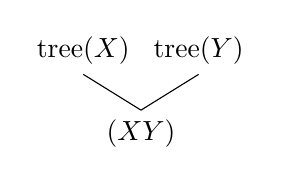
\begin{tikzpicture}[grow'=up]
    \Tree[.$(XY)$ [.{tree$(X)$} ] [.{tree$(Y)$} ] ];
  \end{tikzpicture}
  \hspace{.5in}
  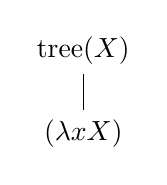
\begin{tikzpicture}[grow'=up]
    \Tree[.$(\l xX)$ [.{tree$(X)$} ] ]
  \end{tikzpicture}
\end{center}
\margnot{Trees Grow Up}{ In Computer Science, trees usually grow down the page from their root node. Our construction trees grow up.}

\examplebox{Example: Construction Tree for $S := (\l x(\l y(\l z((XZ)(YZ)))))$}{
  \begin{center}
    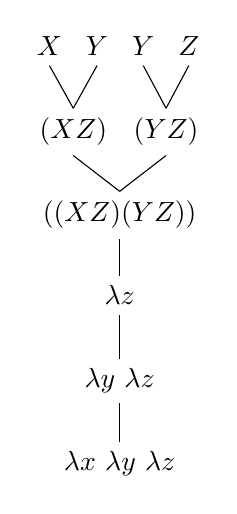
\begin{tikzpicture}[grow'=up]
      \Tree[.$\l x\ \l y\ \l z$ [.$\l y\ \l z$ [.$\l z$ [.$((XZ)(YZ))$ [.$(XZ)$ [.$X$ ] [.$Y$ ] ] [.$(YZ)$ [.$Y$ ] [.$Z$ ] ] ] ] ] ];
    \end{tikzpicture}
  \end{center}
}

%Many terms are defined by recursion on the construction tree.\\

\section{Parenthesis}
\index{Parenthesis|textbf}
At this point in the discussion of the syntax of the lambda calculus, it is worth spending some time talking about parenthesis. We use parenthesis to make explicit and unambiguous what the construction tree for a term looks like. Otherwise, if we came across a term like $\l xXY$, we wouldn't know whether to interpret it as $(\l xX)Y$ or $\l x(XY)$! On the other hand, when we begin to work with longer terms, our notation risks becoming cumbersome if every term must be written with all possible parenthesis. We spend some time now determining the minimum necessary parenthesis necessary to make a term unambiguous so as to save time manipulating cumbersome notation later.

\subsection{Proper Pairings}
A sequence of parenthesis is said to have a \textbf{proper pairing}\index{Proper Pairing} if there exists a bijection $\phi$ from left parenthesis to right parenthesis satisfying two conditions:
\begin{itemize}
  \item $\phi(l)$ is to the right of $l$.
  \item There are no crossings. $(_1(_2)_1)_2$ is bad. $()()$ is okay, and $(_1(_2)_2)_1$ is okay.
\end{itemize}
We claim that the parenthesis of a term are properly paired. We can prove this by induction on the construction tree of a term. If the term is of the form $(x)$, then the parenthesis are properly paired, as there can be no parenthesis inside the variable $x$. If the term is of the form $(XY)$, $(X)$, or $(\l xX)$, then the outermost pair of parenthesis are properly paired if the parenthesis in $X$ and $Y$ are properly paired. We take the case of a single variable as our base case, and see that our induction hypothesis is satisfied, so we are done.\\

\margnot{Connections}{ A sequence of parenthesis can be thought of as a depth-first search of a tree, thinking of a left paren as taking an edge down, and a right paren as taking an edge up.}

We can now also see that if a sequence of parens has a proper pairing, then the sequence is unique. We prove this again by induction. This time, we induct on the number of parenthesis, $n$. If $n = 1$, then it is clear that there is only one proper pairing: $()$.\\

For $n > 1$ we know there must be at least one left paren which begins the sequence. We then have a sequence of zero or more left parenthesis. The first right parenthesis we encounter must be paired with the rightmost left parenthesis:
\begin{equation*}
  (...(_m)_m
\end{equation*}
Observe that there is only one way that this first pairing can be made. $(_m$ must be paired with $)_m$. If this is not the case, then we would have a crossing, which is not allowed in a proper pairing. We remove the $m$ parenthesis, and now we have $2(n-1)$ parenthesis in our pairing. We can then see that the claim is true for all $n$ by induction.\\

\subsection{Checking Whether a Pairing is Proper}
There is a fairly simple algorithm for check whether a pairing is proper. Start with a number $x = 0$ at the left end of the sequence of parenthesis. Every time you encounter a left paren, increment $x$ by 1. Every time you encounter a right paren, decrement $x$ by 1. Throughout this process, if the pairing is proper $n$ will never be negative. The process will terminate with $x = 0$ again.\\

We can prove the correctness of this algorithm as well by induction on the number of pairs of parenthesis, $n$. For $n = 1$, there are only two possible pairings: $()$ and $)($. The first pairing is correct. The sequence of values of $x$ is $0,1,0$. The second pairing has a sequence of $0,-1,0$, so our algorithm claims (correctly) that this pairing is not proper.\\

Now assume that the algorithm is correct for pairings of length $2n$. Our sequence of values for $x$ satisfies the property that the first and last numbers are zero, and that there are no negative numbers in the sequence. We can then add either $0$ or $1$ parens to our list. If we add $1$, then the final value of $x$ will be either $1$ or $-1$, so this make the pairing improper by our algorithm. If we add two parens, and they are unmatched, then TODO: FINISH THIS PROOF
\chapter{Lecture 2}
\lhead{January 14, 2015}
\chead{21-366 Lambda Calculus Lecture 2}

\section{Construction Trees}
\index{Construction Tree|textbf}
During the previous lecture, we proved that proper pairings of parenthesis are unique, and that each term has a proper pairing. We also observed that each term has an associated construction tree. From this we can demonstrate that construction trees are unique.\\

\subsection{Generating Construction Trees}
It is nice to know that unique construction tree representations exist for terms, but it would be useful sometimes to know what those construction trees actually are. We can describe an algorithm that, when given a term, provides the construction tree for that term.\\

\margnot{Note}{ Even though we omit parens sometimes when writing terms, when we prove statements involving parenthesis, we treat the terms as if no parens have been omitted.}

In the most simple case, a term with no parens is a variable. Variables are terminal nodes in our construction tree. If there are parenthesis, then we begin with the leftmost left parent. Since the pairing is proper, this leftmost paren must be paired with the rightmost right paren. Otherwise, a crossing would have occurred. We then have one of three cases: either the first symbol is a variable, the first symbol is a left paren, or the first symbol is a \l. If the first symbol is a variable, then our term is of the form $(xY)$, and has this construction tree:

\begin{center}
  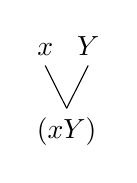
\begin{tikzpicture}[grow'=up]
    \Tree[.$(xY)$ [.$x$ ] [.$Y$ ] ]
  \end{tikzpicture}
\end{center}

$x$ is terminal, so we induct on $Y$. Otherwise, if the next symbol is a left paren, we have a term of the form $((X)(Y))$. We can then induct on both $X$ and $Y$ with the following construction tree:

\begin{center}
  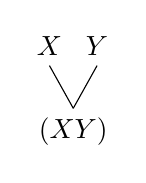
\begin{tikzpicture}[grow'=up]
    \Tree[.$(XY)$ [.$X$ ] [.$Y$ ] ]
  \end{tikzpicture}
\end{center}

In our final case, we have that our term is of the form $(\l xX)$, which has the construction tree:

\begin{center}
  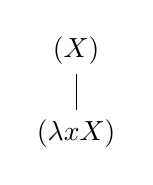
\begin{tikzpicture}[grow'=up]
    \Tree[.$(\l xX)$ [.$(X)$ ] ]
  \end{tikzpicture}
\end{center}

Again, we induct on $X$. From this we can generate a construction tree for any term.\\

\examplebox{Example: Construction Tree for $(\l x(X(xy)))$}{
  We begin by using the rule for constructing a tree from a lambda term:
  \begin{center}
    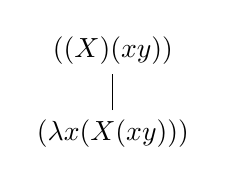
\begin{tikzpicture}[grow'=up]
      \Tree[.$(\l x(X(xy)))$ [.$((X)(xy))$ ] ]
    \end{tikzpicture}
  \end{center}
  We then use the rule for application terms:
  \begin{center}
    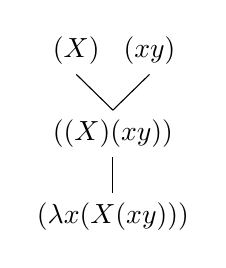
\begin{tikzpicture}[grow'=up]
      \Tree[.$(\l x(X(xy)))$ [.$((X)(xy))$ [.$(X)$ ] [.$(xy)$ ] ] ]
    \end{tikzpicture}
  \end{center}
  Finally, we treat the $X$ path as completed, since we havedn't defined what $X$ is, and use the application rule once more on the $(xy)$ path:
  \begin{center}
    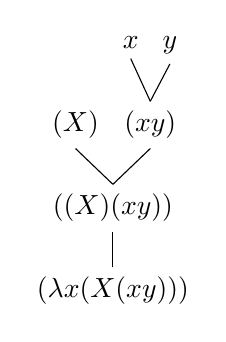
\begin{tikzpicture}[grow'=up]
      \Tree[.$(\l x(X(xy)))$ [.$((X)(xy))$ [.$(X)$ ] [.$(xy)$ [.$x$ ] [.$y$ ] ] ] ]
    \end{tikzpicture}
  \end{center}
}



\section{Some Definitions}
It is somewhat cumbersome to always have to write ``a term of the form $(XY)$'' when we want to talk about subtermsof an application. When we have a term of the form $(XY)$, we say that $X$ is in \textbf{function position}\index{Function Position}, and $Y$ is in \textbf{argument position}\index{Argument Position}. We also say that $Y$ is applied to $X$.\\

\subsection{Subterms}
\index{Subterm|textbf}
Let $Y$ be a term. $Y$ is a subterm of $X$ if $Y$ is also a substring of $X$, with the exception of a variable following a \l.\\

\noindent\textbf{Trichotomy Law: }\index{Trichotomy Law} Given any two subterm occurances\footnote{In this course, subterm occurances will be notated with primes.} $Y',Z'$ of a term $X$, then either they are disjoint or one contains the other.\\

\subsection{Free and Bound Variables}
\index{Free Variable|textbf}\index{Bound Variable|textbf}
In a lambda term $(\l x.X)$, we say that the variable $x$ is \textbf{bound} by the term, because the contents of the term will be determined by the argument provided to the lambda. Variables which are not bound in this way are called \textbf{free.} It is possible for variables to be free in one term, but bound by a term which occurs higher in the construction tree. It should be clear, for example, that the term $x$ has one free variable: $x$ itself. However in the term $\l x.X$, it is bound by the lambda.\\

So, what happens to bound and free variables when we have a term of the form $(XY)$? Since there are no lambdas introduced, the status of the variables cannot change. The variables which were bound remain bound, and the variables which are free remain free. We can summarize the rules for determining which variables are bound and which are free as follows:\\

\examplebox{Summary of Bound and Free Variables}{
\begin{eqnarray*}
  FV(x) &=& \{x\}\\
  BV(x) &=& \emptyset\\
  FV((XY)) &=& FV(X) \cup FV(Y)\\
  BV((XY)) &=& BV(X) \cup BV(Y)\\
  FV((\l xX)) &=& FV(X) - \{x\}\\
  BV((\l xX)) &=& BV(X) \cup \{x\}\\
\end{eqnarray*}
}

It is useful when attempting to determine which variables of a term are bound and which are free by hand, to draw the construction tree for the term. It is obvious what variables in the roots of the tree are bound, and which are free. From there, the recursive definitions given above can be employed.\\

\examplebox{Example: Determining the Bound Variables of a Term}{
  Say that we have a term $((xx)(\l x.(xx)))$ for which we want to determine the free variables. We begin by drawing the construction tree:
  \begin{center}
    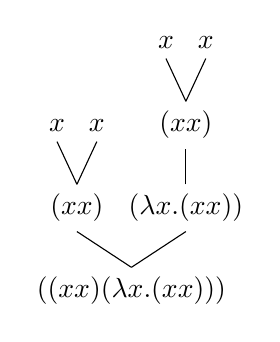
\begin{tikzpicture}[grow'=up]
      \Tree[.$((xx)(\l x.(xx)))$ [.$(xx)$ [.$x$ ] [.$x$ ] ] [.$(\l x.(xx))$ [.$(xx)$ [.$x$ ] [.$x$ ] ] ] ]
    \end{tikzpicture}
  \end{center}
  All of the root nodes of the tree are terms $x$, which have free variables $x$. Both terms of $(xx)$ are of the form $(XY)$, so their free variables are the union of the free variables of their subtrees, or $x$. The lambda term $\l x.xx$ binds $x$, so $x$ is no longer free. The top term inherits the free and bound variables of its subtrees once more, so the bound variables are $x$, and the free variables are... $x$.
}

The example above illustrates a subtlety which is easy to miss. The variable $x$ in the left subtree is not the same as the variable $x$ in the right subtree. We wrote them as the same symbol, but in actuality they are wholly unrelated. If we represent the $x$s in the left subtree as $y$s instead, the situation makes itself clear.

\begin{center}
  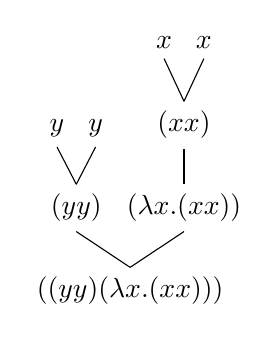
\begin{tikzpicture}[grow'=up]
    \Tree[.$((yy)(\l x.(xx)))$ [.$(yy)$ [.$y$ ] [.$y$ ] ] [.$(\l x.(xx))$ [.$(xx)$ [.$x$ ] [.$x$ ] ] ] ]
  \end{tikzpicture}
\end{center}

The free variables are $y$, and the bound variables are $x$.

\section{Minimizing Parenthesization}
\margnot{Jan \L usckasevicz}{ Jan was born in 1878 in Poland. He worked in analytical philosophy and logic. He is best known for Polish notation.}
We've talked a bit so far about ways to reduce the number of parenthesis needed to unambiguously determine the construction tree of a term. Now we will formally introduce three strategies for removing parenthesis: Polish notation, Church's dot notation, and left associative deletion.

\subsection{Polish Notation}
\index{Polish Notation}


\margnot{Polish Notation}{ Polish notation is sometimes referred to in other contexts as ``prefix notation.'' Equivalently, there is a ``postfix notation'' which is sometimes called Reverse Polish Notation.}

Polish notation was invented by Jan \L uckasevicz\index{Lusckasevicz, Jan@\L usckasevicz, Jan} in 1924. We use only the symbols $\l$ and $($, plus variables $x,y,z$ and terms $X,Y$. The key feature of Polish notation is that operators are placed before their arguments. Take, for example, the expression $3 + 4$. The operator in this expression, the $+$ occurs between the arguments, $3,4$. In Polish notation, we would instead write $+ 3 4$. In this simple case it is not immediately obvious what is gained by this. When we try it on a larger expression, it becomes clear what the advantage is:
\begin{equation*}
  ((3 + 4) \times (2 + 2)) / (1 + 5) \Rightarrow / \times + 3\ 4 + 2\ 2 + 1\ 5
\end{equation*}
Notice how by rearranging the expression, we can remain unambiguous without parenthesis. We can adopt a similar style for writing lambda terms. We use the terms $\l,(, x, y, z$ where $x, y, z$ are variables, and $X,Y$ are terms.\\

\examplebox{Example: Lambda Terms in Polish Notation}{
  \begin{eqnarray*}
    (XY\\
    \l xX
  \end{eqnarray*}
}

We can notice that terms written using Polish notation can be fairly straightforwardly derived from terms which do not, simply by omitting the right parens. Although this does significantly reduce the number of necessary parenthesis, it also makes the terms much more difficult to read, so we will not actually use this method in practice.

\subsection{Church's Dot Notation}
\index{Church, Alonzo!Church's Dot Notation|textbf}
\margnotTwo{Willard Van Orman}{Quine}{ Born in 1908, the American philsopher and logic Quine spent his life at Harvard University.}

Another convention we can use is a dot notation developed by Quine\index{Quine, Willard Van Orman}, called Church's dot notation. Using this notation, we take a term with some number of initial lambdas, and remove the parens around all of them, placing a dot after the last one. So if we have an expression of the form
\begin{equation*}
  (\l x_1(\l x_2(\l x_3\ldots(\l x_nX)\ldots)))
\end{equation*}
We can write it as
\begin{equation*}
  (\l x_1x_2\ldots x_n.X)
\end{equation*}
This makes it much easier to write out functions which take in multiple arguments as lambda terms. It is worth mentioning currying again here. Writing a curried function in dot notation might make it seem like we are again working with functions which take in multiple arguments again. We are not.

\examplebox{Example: Dot Notation Representation of $S$}{
  \begin{equation*}
    S := (\l x (\l y (\l z((xy)(yz))))) = \l xyz.((xy)(yz))
  \end{equation*}
}

\subsection{Left Association}
\index{Left Association|textbf}
We can delete all of the parenthesis around applications where the subterm is not in argument position. So in a term $(XY)$, we can delete parens around $X$, if any occur. We also retain the outermost set of parenthesis in a formal sense, although we will tend to omit them in practice. So if $X = (UV)$ and we have a term $((UV)Y)$ we would delte the parenthesis around $(UV)$ to get $(UVY)$.

\examplebox{Example: Left Association Representation of $S$}{
  \begin{equation*}
    S := (\l x (\l y (\l z((xy)(yz))))) = (\l x (\l y (\l z(xy(yz)))))
  \end{equation*}
}

It is not immediately obvious that this strategy for deleting parenthesis preserves uniqueness. This is proven in the next lecture.

\section{Proper Extensions}
\index{Proper Extension|textbf}
We say that a string $s_1$ is a proper extension of some string $s_2$ if $s_1$ can be written as the concatenation of $s_2$ and another nonempty string. The string ``Hello world'' is therefore a proper extension of the string ``Hello'' by the concatenation of the extra string `` world''. We claim that no term is a proper extension of another term as a string read from left to right.\\

We can prove this by induction on the sum of the lengths of the two sequences. The smallest sequence is a variable $x$. No term can be an extension of a variable because a left paren is necessary. Now consider a term $X$ with an extension $Y$. There are two possible cases: either $X$ is of the form $X = \l uU$ or $X = (UV)$.\\

If $X = \l uU$, then the only way to extend $X$ is if $Y$ begins with $\l u$, which can only be extended into a term of the form $\l uV$. Since we claim by our induction hypothesis that $V$ is not a proper extension of $U$ for ally $U$, $V$ smaller than $X$,$Y$, and $U$ must necessarily be an extension of $U$, we have a contradiction.\\

In our other case, we have that $X = (UV$. Therefore $Y$ must begin with a paren, and so be of the form $Y = (ZW$. This implies that $ZW$ is an extension of $UV$. By our induction hypothesis, $U = Z$ and $V = W$, so there can be no extension. So construction trees are unique.
\chapter{Lecture 3}
\lhead{January 16, 2015}
\chead{21-366 Lambda Calculus Lecture 3}

\section{Left Association Deletion of Parens}
In the previous lecture, we asserted that we could take all of the parenthesis around terms which were not in argument position away without violating the uniqueness of the term. Let $X$ be a term. We define $X^*$ as the result of the left associative deletion of parenthesis from $X$. We show here what left associative deletion looks like for various terms. Later, in our uniqueness proof, we will refer back to these example terms.\\

\begin{eqnarray*}
  (1) &=& x\\
  (2) &=& (\l x_1 \ldots x_n . x_i)\\
  (3) &=& (\l x_1 \ldots x_n.((\l xX_0)X_1) \ldots )X_m))\\
  (4) &=& (\underbrace{\l x_1 \ldots x_n}_{\hbox{Lambda prefix}} . \underbrace{(( \ldots (\underbrace{x_i}_{\hbox{head}} X_i) \ldots )X_m )}_{\hbox{matrix}}\\
\end{eqnarray*}

\margnot{Illustration of 3 and 4}{
\begin{center}
  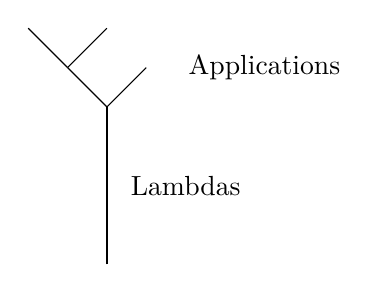
\begin{tikzpicture}
    \draw (0,0) -- (0,2);
    \draw (0,2) -- (.5, 2.5);
    \draw (0,2) -- (-.5, 2.5);
    \draw (-0.5, 2.5) -- (-1, 3);
    \draw (-0.5, 2.5) -- (0, 3);

    \draw (1,1) node {Lambdas};
    \draw (2,2.5) node {Applications};
  \end{tikzpicture}
\end{center}
}

Left association deletion for case $(1)$ is trival. There are no parenthesis at all, so we delete nothing. In case $(2)$, we have a sequence of lambdas followed by a single application. This does not have any parenthesis around subterms which are not in argument position, so again we cannot delete any parenthesis. Case $(3)$ is the first case where we can delete something. The term at the head of the application is of the form $((\l xX_0)X_1)$, which can be reduced to $(\l xX_0X_1)$. In case 4, the first subterm is of the form $((x_i X_i)\ldots)$. The innermost parens here can be removed, giving another term which has parenthesis around the subterm not in argument position. By repeating this process, $(4*)$ is derived.

\begin{eqnarray*}
  (1*) &=& x\\
  (2*) &=& (\l x_1\ldots x_n.x_i)\\
  (3*) &=& (\l x_1 \ldots x_n . (\l xX_0X_1 \ldots X_m)\\
  (4*) &=& (\l x_1 \ldots x_n . x_LX_1 \ldots X_m)\\
\end{eqnarray*}

\subsection{Proof of Uniqueness}
Our claim is that $X \not= Y$ if and only if $X^* \not= Y$. There are four possible cases for the form of our terms $X$ and $Y$. We will prove the claim by induction on $X$. Our base case is $X$ as a variable. It is either of the form $((x)y)$ or $(x(y))$, or a single variable $z$, where $x, y$ and $z$ could have subterms.\\

Our first case is that $X := z$. It has no parens, so we are done. If it is of the form $((xy)z)$ or $(x(yz))$, however, we can evaluate $((xy)z)*$ and $(x(yz))*$:
\begin{eqnarray*}
  ((xy)z)* &=& xyz\\
  (x(yz))* &=& x(yz)\\
\end{eqnarray*}
We can say that we can uniquely restore the parens, based on whether we are in the first or second listed case.\\

Induction Step: In case (2), we have two parens. This can only happen the two parens are the outermost parens around the term:
\begin{equation*}
  (\l x_1 \ldots x_n.X_{i_1}\ldots X_{i_k})
\end{equation*}
In our left association deletion scheme, we do not delete outermost parens, so the term remains unchanged. If all of the variables can be uniquely restored, then case $(2)$ can be uniquely restored as well.\\

$X^* = Y^*$ in cases where $(1)^*, (2)^* \Rightarrow X = Y$.\\

Consider the proper pairing of parens. Case (2) applies to $X$ implies (2) applies to $Y$ and case (3) applies to $X$ implies (3) applies to $Y$.
\begin{equation*}
  (\l x_1 \ldots x_n (\l xX_0))(\ \ \ )(\ \ \ ))
\end{equation*}
The parens in argument position must be reconstructable by the induction hypothesis. FIGURE OUT AND FIX THIS PROOF.

\section{Substitution of a Term for a Variable}
A problem arises when we attempt to substitute one term into another where both terms contain the same variables. The problem is that it is ambiguous which variables mean what when both are represented by the same symbol. Take for example the following application:
\begin{eqnarray*}
  (\l x . yx)(zx)\\
  (\l x . y(zx))\\
\end{eqnarray*}
When we make this application, we have $x$s both before and after the application, but the $x$s mean different things. In this simplified example, it can be figured out what is going on by manual inspection, but it gets worse when the terms are more complicated. We therefore have an incentive to resolve this naming issue before then. An easy solution is to simply change the name of the symbol in the lambda:
\begin{eqnarray*}
  (\l u . yu)\\
  (\l u . (zx)u)
\end{eqnarray*}
TODO: THIS IS WRONG. WHY.

\subsection{Clash Graphs}
\index{Clash Graph|textbf}
We have some abstract term. From the root, there is only one path to any given leaf.
\begin{center}
  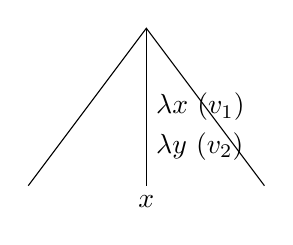
\begin{tikzpicture}
    \draw (0,0) -- (0,-1) node[anchor=west] {$\l x\ (v_1)$};
    \draw (0,-1) -- (0,-2) node[anchor=north] {$x$};
    \draw (-1.5,-2) -- (0,0) -- (1.5,-2);

    \draw (0,-1.5) node[anchor=west] {$\l y\ (v_2)$};

    % Draw an arrow from x to \l x.
  \end{tikzpicture}
\end{center}

We define a \textbf{clash graph} which has verticies that are the \l{} abstraction nodes of the term. $v_1$ is adjacent to $v_2$ provided that $v_2$ lies on the path from $v_1$ to a leaf which it binds, or vice versa.

\chapter{Lecture 4}
\lhead{January 21, 2015}
\chead{21-366 Lambda Calculus Lecture 4}

\section{Substitution}
\index{Substitution|textbf}

We have been talking about the idea of substitution for a while now, so it's time to formally describe what we mean. Let $X$ be a term with subterm $x$. We say that we are substituting $Y$ for $x$ in $X$ to mean that we are replacing every occurance of $x$ in the construction tree of $X$ with $Y$. We notate this with Curry's\index{Curry, Haskell} substitution prefix\index{Curry, Haskell!Curry's Substitution Prefix}: $[X / x]Y$ read ``substitute $X$ for each free occurance of $x$ in $Y$.'' We call the substitution of a single term a \textbf{single substitution}.\\

\examplebox{Effects of Substitutions}{
  \begin{eqnarray*}
    {[X / x]}x &=& X\\
    {[X / x]}y &=& y\\
    {[X / x]}(UV) &=& ([X / x]U [X /x]V)\\
    {[X /x]}(\l uU) &=& \l u[X / x]U\ \ (u \neq x)\\
    {[X / x]}(\l xU) &=& \l xU\\
  \end{eqnarray*}
}

It is possible to perform multiple substitutions at once. We call this \textbf{simultaneous substitution}. A simultaneous substitution is notated by $[X_1/x_1,\ldots,X_n/x_n]Y$. We can also set an order for the substitutions which are performed by writing an expression of the form $[X_{n-1}/x_{n-1}]([X_n / x_n]Y)$, which we call a \textbf{sequential substitution}.\\

It is important to note that simultaneous and sequential substitutions do not necessarily produce the same result. This is because the first substitution to be applied is then substituted by the second, and so on.
\begin{eqnarray*}
  [U/u]([V/v]Y) &=& [U/u,[U/u]V/v]Y\\
\end{eqnarray*}

\examplebox{Example: A Substitution both Simultaneous and Sequential}{
  Take the substitution of $X/x$ and $Y/X$ into the term $x$. We can see that the simultaneous substitution is
  \begin{equation*}
    [X/x,Y/X]x = X
  \end{equation*}
  while the sequential substitution is either
  \begin{equation*}
    [X/x]([Y/X]x) = X
  \end{equation*}
  or
  \begin{equation*}
    [Y/X]([X/x]x) = Y
  \end{equation*}
  depending on the order in which the substitutions are applied.
}

\section{What to do about Bound Variables?}
We have the clash graph of an abstract term. Verticies are occurances of \l's in the term. An edge is between two adjacent \l's. What does it mean to assign new variables to the \l's and maintain the same abstract term such that no two \l's that are adjacent get the same variable? It affects all the variables which are bound by that \l.\\

Any free variables can be bound by adding more \l's at the top. This is called a \textbf{closure}.\\
\index{Closure}

We can think of renaming the variables of the term $\l [X / x]U$ as attempting to color a graph. How many colors do we need?\\

A \textbf{clique}\index{Clique} in a graph is a set of verticies such that any 2 are adjacent.
%\begin{tikzpicture}
  % Clique | Non-Clique
  % o | 
  % o--o | o  o
  % through size 5. Note that size 5 requires one line to jump.
%\end{tikzpicture}
If a graph has a clique of size $n$, then you need $n$ colors to color the graph. The converse of this statement is not true. Take for example the graph of a pentagram. It has cliques of size 2, but requires 3 colors to color it.\\% Add picture here

\subsection{How to rewrite a term's bound variables}
Notice that if we take any \l{} which is closest to the frontier\footnote{That is, that it has no \l's below it.}, then all things which are adjacent to it lie above it. Now if we take any clique in the clash graph, and take any \l{} in that clique which is as close to the frontier as possible, all things adjacent to it lie above it. Additionally, all of them are adjacent to each other.\\

We take the largest clique in the clash graph, and take the lowest possible \l{} and remove it. We now have a term in one less \l. Suppose now that we can rewrite the entire term with the \l{} deleted. We can do this by rewriting the bound variables recursively. If we have another clique of size $n$, we can color our lowest \l{} with the color $x$ and we then have to color the rest of the clique with $n - 1$ colors, giving us $n$ total colors. If we do not have another clique of size $n$, then we can color our lowest \l{} with $x$ and again color the rest with $n - 1$ colors. Thus our maximum number of colors is the size of the largest clique in the clash graph.\\

\section{Equivalence Relations on Terms}
\index{Equivalence Relation|textbf}
Intuitively, an equivalence relation on a set is a function $f: (a,b) \mapsto \{\hbox{true},\hbox{false}\}$ which is true only if $a$ is ``equal'' to $b$ in some way. More precisely, if the set is partitioned in some way, then an equivalence relation is true only if the two elements are in the same subset of the partition.\\

An equivalence relation $f$ satisfies the following properties:
\begin{itemize}
  \item \textbf{Identity Property:} An element $a$ is equivalent to itself.
    \begin{equation*}
      (f(a,a) = \hbox{true})
    \end{equation*}
  \item \textbf{Symmetric Property:} If and only if an element $a$ is equivalent to some other element $b$, then $b$ is equivalent to $a$.
    \begin{equation*}
      f(a,b) = f(b,a)
    \end{equation*}
  \item \textbf{Transitive Property:} If $a$ is equivalent to $b$ and $b$ is equivalent to $c$, then $a$ is equivalent to $c$.
    \begin{equation*}
      f(a,b),f(b,c)\Rightarrow f(a,c)
    \end{equation*}
\end{itemize}

\subsection{Alpha Conversion}
\index{Alpha Conversion|textbf}
Two terms $X$ and $Y$ are $\alpha$ equivalent if one can be derived from the other by changing bound variables. This derivation is called $\alpha$ conversion. The simplest case of alpha conversion is that where $X = \l x X$ and $Y = \l y X$. It is clear that you can convert $X$ into $Y$ by simply replacing the bound variable $x$ with the bound variable $y$. An $\alpha$ conversion which changes only a single bound variable is called an elementary $\alpha$ conversion.\\

The $\alpha$ equivalence relation clearly satisfies the identity property. Any term can be converted into itself by changing no bound variables. It also satisfies the symmetric property. Any $\alpha$ conversion can be undone, and the conversion which undoes it proves the relation in the opposite direction. That is, a conversion from $X$ to $Y$ can be reversed to create a conversion from $Y$ to $X$ by changing the variables back. Finally, the $\alpha$ equivalence relation satisfies the transitive property. Take some terms $X, Y$ and $Z$ such that $X$ and $Y$ are alpha equivalent and $Y$ and $Z$ are alpha equivalent. This implies that there is a conversion from $X$ to $Y$ and a conversion from $Y$ to $Z$. We can convert $X$ into $Y$ and then into $Z$ using those two conversions, demonstrating that $X$ can be converted into $Z$. This satisfies the equivalence between $X$ and $Z$.\\

$\alpha$ conversions are not particularly difficult to grasp or work with, so this is the only time we will really talk about them. It is useful, though, to know that the names we give to things do not affect how they behave.\\

\subsection{Eta Conversion}
\index{Eta Conversion|textbf}
Our second equivalence relation is $\eta$ equivalence. Two terms $U$ and $V$ are $\eta$ equivalent if (without loss of generality) $U = \l x(Xx)$ and $V = X$. A conversion from $U$ to $V$ is called an $\eta$ reduction, and a conversion from $V$ to $U$ is called an $\eta$ expansion.\\
\examplebox{$\eta$ expansion and reduction}{
  \begin{center}
    \begin{tabular}{c @{\hspace{.75in}} c}
      $ X \rightarrow_\eta \l x(Xx)$ & $\l x(Xx) \rightarrow_\eta X$\\
      $\eta$ expansion & $\eta$ reduction\\
    \end{tabular}
  \end{center}
}

For the sake of our equivalence relation, we say that a term is $\eta$ equivalent to itself.\\

Like with $\alpha$ equivalence, we are not going to talk about $\eta$ conversion much, at least for the first half of the course. In the second half, it will come up again. This is because there really isn't much to $\eta$ conversion.

\subsection{Beta Conversion}
\index{Beta Conversion|textbf}
We hinted earlier at the fact that we could create something analogous to functions in lambda calculus. The mechanism by which this happens is called $\beta$ conversion, and it allows substitution in terms. The equivalence relation for $\beta$ conversion is based on the following transformation:
\begin{equation*}
  (\l xX)Y \rightarrow_\beta [Y/x]X
\end{equation*}
In this transformation, we call $(\l xX)Y$ the \textbf{redex}. Curry called the $[Y/x]X$ term the \textbf{reducant} or \textbf{contractant}, but we will refer to them much, if at all.

\textbf{Remark:} General $\beta$ conversion. We define as a $\beta$ redex as the term $(\l xX)Y$. Curry defined $[Y /x]X$ as the reductant or contractant. We will not use these terms. $\beta$ reduction can be represented as:
\begin{equation*}
  (\l xX)Y \rightarrow_\beta [Y / x]X
\end{equation*}
We allow ourselves to do this inside of bigger terms. We can $\beta$ reduce\index{Beta Reduction} a small term inside a bigger term to $\beta$ reduce the entire term.\\

The equivalence relation $\beta$ conversion is based on the following: $(\l xX)Y =_\beta [Y / x]X$. This is analogous to the example of having a polynomial $p(x) = a_0 + a_1x + \ldots + a_nx^n$, and evaluating it at a point:
\begin{equation*}
  \hbox{Eval}(p(x),\pi) = a_0 + a_1\pi + a_2\pi^2 + \ldots + a_n\pi^n
\end{equation*}
\chapter{Lecture 5}
\lhead{January 23, 2015}
\chead{21-366 Lambda Calculus Lecture 5}

% Make Peaks and Valleys in beta redution pictures.
\section{Reductions}
Note that we hide $\alpha$ conversions while we do more interesting things. We will also concentrate on $\beta$ reduction.\index{Beta Reduction} $\eta$ reduction\index{Eta Reduction} is somewhat trivial.
\subsection{$\beta$ Reduction}
\begin{equation*}
  \underbrace{(\l xX)Y}_{\hbox{Redex}} \rightarrow_\beta \underbrace{[Y / x]X}_{\hbox{reductum}}
\end{equation*}
\index{Redex}\index{Reductum}
{\begin{center} $\rightarrow$ contraction $\rightarrow$ \end{center}}
\subsection{$\eta$ Reduction}
\begin{equation*}
  \underbrace{\l x(Xx)}_{\hbox{redex}} \rightarrow_\eta \underbrace{X}_{\hbox{reductum}} \hspace{.5in} x \not\in FV(X)
\end{equation*}
 Additionally note that we call it ``reduction,'' but it is entirely possible that the reductum is equal in length to or longer than the redex. For example:
\begin{eqnarray*}
  1)\ (\l x x)Y &\rightarrow_\beta& Y\\
  2)\ (\l xy.x)YZ &\rightarrow_\beta& (\l yY)Z\\
  (\l x (\l yx))Y &\rightarrow_\beta& [Y/x](\l yx) = \l yY\\
  &\rightarrow_\beta& Y
\end{eqnarray*}

\subsection{$\omega$ and $\Omega$}
We now introduce a pair of term $\omega$ and $\Omega$ which often come up as the counterexamples to otherwise true claims in lambda calculus.
\begin{eqnarray*}
  \omega &:=& \l x (xx)\\
  \Omega &:=& (\omega\omega) = (\l x(xx))(\l x(xx))
\end{eqnarray*}
\textbf{Definition:} If $FV(X) = \emptyset$, then $X$ is said to be \textbf{closed,} or a \textbf{combinator.}\index{Combinator} (Here we can also say that $X$ is a closure.) Now we define a step beyond $\Omega$:
\begin{eqnarray*}
  \Omega^+ := (\l x (xxx))(\l x (xxx))
\end{eqnarray*}
What happens if we apply $\Omega^+$ to itself?
\begin{equation*}
  \Omega^+\Omega^+ \rbeta (\Omega^+\Omega^+)\Omega^+ \rbeta \Omega^+\Omega^+\Omega^+\Omega^+
\end{equation*}

We can also refer to situations where the redex is inside a larger term as a beta reduction. Imagine that $U$ has a subterm $(\l x X)Y$. We can write that $U \rbeta V$ when $V$ has a subterm $[Y/x]Y$. So beta reduction can occur on subterms.\\

Interestingly, if you are given $U$ and $V$, and that $U \rbeta V$, you cannot tell what subterms are being reduced. The (essentially only) counterexample is $\Omega$:
\begin{equation*}
  x\Omega\Omega \rightarrow x\Omega\Omega
\end{equation*}

Now we want to generalize this to many steps. This is called a \textbf{transitive closure.} We notate transitive closure\index{Transitive Closure} as
\begin{equation*}
  U \twoheadrightarrow V
\end{equation*}
if there exists a sequence $U = U_0 \rbeta U_1 \rbeta \cdots \rbeta U_n = V$. $n$ can be zero, in which case $U = V$, and we allow $U$ to reduce to itself. This is conventional, and it doesn't hurt anything.\\

We say that $U =_\beta V$ (read as $U$ is beta equivalent\index{Beta Equivalent} to $V$) if there exists a sequence $U = U_0 \cdots U_{n-1} U_n = V$ such that
\begin{equation*}
  U_0 \twoheadrightarrow_\beta U_1 \twoheadleftarrow_\beta U_2 \twoheadrightarrow_\beta U_3 \cdots \twoheadleftarrow_\beta U_{n-1} \twoheadrightarrow_\beta U_n = V
\end{equation*}
Note that beta equivalence is transitive:
\begin{equation*}
  U =_\beta V, V =_\beta W \Rightarrow U =_\beta W
\end{equation*}
Example of beta equivalence:
\begin{eqnarray*}
  (\l xy.x)\Omega\Omega \twoheadrightarrow_\beta \Omega \twoheadleftarrow_\beta (\l xy.x)\Omega\Omega^+
\end{eqnarray*}
We can therefore say that $(\l xy.x)\Omega\Omega =_\beta (\l xy.x)\Omega\Omega^+$.\\

TODO: MAKE SURE $K$ IS DEFINED IN A NOTICEABLE WAY. IT IS REFERENCED LATER.\\
Another example: Let $K := \l xy.x$ and $I := \l x.x$
\begin{equation*}
  \omega K \omega \twoheadrightarrow_\beta (KK)\omega \twoheadrightarrow_\beta K \twoheadleftarrow_\beta IK
\end{equation*}

A third example: $xXY$. If $X \rbeta X^+$ and $Y \rbeta Y^+$.
\begin{equation*}
  xXY^+ \twoheadleftarrow_\beta xXY \twoheadrightarrow_\beta xX^+Y
\end{equation*}

\section{Properties of Beta Equivalence}
Beta equivalence satisfies the properties of an equivalence relation.
\begin{itemize}
  \item $U =_\beta U$
  \item if $U =_\beta V$ then $V =_\beta U$
  \item if $U =_\beta V$, $V =_\beta W$, then $U =_\beta W$
\end{itemize}
We then have the following properties:
\begin{enumerate}
  \item $(\l x X)Y \twoheadrightarrow_\beta [Y/x]X$
  \item if $X \twoheadrightarrow_\beta Y$, $U \twoheadrightarrow_\beta V$, then $(XU) \twoheadrightarrow_\beta (YV)$.
  \item if $X \twoheadrightarrow_\beta Y$, then $(\l xX) \twoheadrightarrow_\beta (\l xY)$.
\end{enumerate}
Similar properties hold for $=_\beta$ as do for $\twoheadrightarrow_\beta$.

\section{Redex Creation}
We take a term $U$ with subterm $(\l xX)Y$, and create a term $V$ with subterm $[Y/x]X$. Old redexes have 0 or more residuals in $V$. Now we peek into $X$: $(\l xX)Y$ is actually $((\l x(\l zZ))Y)W$. We can contract it into $(\l z[Y/x]Z)$.

\section{The Church-Rosser Theorem}
\index{Church-Rosser Theorem}
%Actually proven by Church, Rosser, and Kleene.
Does the order in which we perform reductions on a lambda expression matter? This is an important question. If different orders of reduction could be applied to lambda terms to achieve different results, this would have uncomfortable implications for lambda calculus as a model for computation.\\

Imagine that we had a term $X$ which reduced to two separate terms $X'_1$ and $X'_2$ depending on the order in which reductions are applied. We must have that $X'_1 \not= X'_2$, otherwise we could simply reduce one into the other. But we also have that $X = X'_1$ and $X = X'_2$. By transitivity, this implies that $X'_1 = X'_2$, which contradicts our assumption. This contradiction would be a problem. The proof that this contradiction does not occur was published in $1936$ by Alonzo Church and J. Barkley Rosser.\\

\margnot{Church and Rosser's Paper}{ Church and Rosser published this proof as ``Some Properties of Conversion'' in the journal \textit{Transactions of the American Mathematical Society}. It is available at \footnotesize\texttt{http://www.jstor.org/ stable/1989762}}

\examplebox{The Church-Rosser Theorem}{ If $X =_\beta Y$, then there exists a term $Z$ such that $X \twoheadrightarrow_\beta Z$ and $Y \twoheadrightarrow_\beta Z$. Graphically, we can draw this relationship as:
\begin{center}
  \begin{tikzpicture}
    \draw (0,0) node {$X$};
    \draw (1,1) node {$X_1$};
    \draw (2,0) node {$X_2$};
    \draw (3,1) node {$X_3$};
    \draw (4,0) node {$\ldots$};
    \draw (5,1) node {$X_{n-2}$};
    \draw (6,0) node {$\hphantom{xx}X_{n-1}$};
    \draw (7,1) node {$X_{n}$};
    \draw (8,0) node {$Y$};

    \draw[thick,->] (0.2,0.2) -- (0.8,0.8);
    \draw[thick,<-] (1.2,0.8) -- (1.8,0.2);
    \draw[thick,->] (2.2,0.2) -- (2.8,0.8);
    \draw[thick,<-] (3.2,0.8) -- (3.8,0.2);
    \draw[thick,->] (4.2,0.2) -- (4.8,0.8);
    \draw[thick,<-] (5.2,0.8) -- (5.8,0.2);
    \draw[thick,->] (6.2,0.2) -- (6.8,0.8);
    \draw[thick,<-] (7.2,0.8) -- (7.8,0.2);

    \draw[thick,dashed,->>] (0.2,-0.2) -- (3.8,-3.8);
    \draw[thick,dashed,->>] (7.8,-0.2) -- (4.2,-3.8);

    \draw (4,-4) node {$Z$};
  \end{tikzpicture}
\end{center}
In the above picture, solid arrows represent existing $\beta$ conversions, which might be empty (that is, they might be of the form $X \rightarrow_\beta X$.) Dashed arrows represent $\beta$ conversions which are implied by the theorem.
}

\subsection{Proof of Church-Rosser}
Our proof of the Church-Rosser theorem is based on the intuition that if we could somehow convert ``peaks'' in our diagram into ``valleys,'' we could construct the reductions $X \twoheadrightarrow_\beta Z$ and $Y \twoheadrightarrow_\beta Z$.\\

We first look at techniques for creating new redexes from old redexes. We have some term $U$ such that $\Delta := (\l xX)Y$ is a subterm of $U$. We can contract with beta reduction this term into a $V$ such that $[Y/x]X$ is a subterm of $V$. Now consider another subterm $\Gamma$. There are three cases:\\

\textbf{Case 1:} $\Delta \subset \Gamma$\\
$\Gamma'$ reappears in $V$ as a redex we call the \textit{residual} of $\Gamma$.\\

\textbf{Case 2:} $\Delta$ disjoint from $\Gamma$\\
If they are disjoint, then $\Gamma$ is contained in $U$ and $V$, and $\Gamma$ is its own residual.\\

\textbf{Case 3:} $\Gamma \subset \Delta$\\
\textbf{Subcase 3.1:} $\Gamma \subseteq Y$\\
$\Gamma$ may have many residuals in $V$. There is also the possibility that $x$ does not occur at all in $X$, and there are no residuals. So $\Gamma$ can have zero or more residuals in $V$.\\
\textbf{Subcase 3.2:} $\Gamma \subseteq \l xX$\\
$\Gamma$ now looks like $[Y/x]\Gamma$. If $\Gamma$ has $x$ as a free variable, then the residual of $\Gamma$ is $[Y/x]\Gamma$.\\
\chapter{Lecture 6}
\lhead{January 26, 2015}
\chead{21-366 Lambda Calculus Lecture 6}

\def\uwavy#1{#1}

\section{Computing With $\l$ Terms}
To perform computations, we need data structures. How do we represent data structures? We can use collections of terms that look like data structures. Our target for this lecture is to define the nonnegative integers, booleans, and finite sets. Once we have described these data structures, we can define some operations on them. Specifically, we will define addition and subtraction for the integers, and the conditional operator which branches between two terms dependant on whether a boolean is true or false.

\section{Data Structures}

\subsection{Booleans}
\index{Boolean|textbf}
The way that we define booleans at first may seem a little bit strange. The reason that we define them in the way that we do is motivated by the common use cases for booleans. Often, we want to use booleans inside conditional statements, to decide which of two branches to take. We might write, for example, the following program:
\begin{center}
  \begin{lstlisting}[language=C,backgroundcolor=\color{txtbkpaleblue},showstringspaces=false]
    int age = keyboard.read();
    if (age >= 21) {
      print("Welcome to the bar!");
    }
    else {
      print("Come back when you are older.");
    }
  \end{lstlisting}
\end{center}

One way to do this is to establish an application $(XY)$ where $X$ is the term you would like to evaluate in the case where your boolean is true, and $Y$ is the term you would like to evaluate in the case where your boolean is false.\\

So, in our above example, we would have a term representing the function \texttt{print("Welcome to the bar!")} as $X$ and \texttt{print("Come back when you are older.")} as $Y$. We could then represent the booelan true as the function $(\l xy.x)$ and the boolean false as the function $(\l xy.y)$. We define $K := \l xy.x$ as our true boolean, and $K_* := \l y.xy$ as our false boolean.\\

Typically, if we have some term $T$, we write $T_* := TI$. This is where our notation for $K_*$ is derived. We can demonstrate that $K_* =_\beta KI$ by $\beta$ conversion:
\begin{equation*}
  KI = (\l xy.x)I \rightarrow_\beta Iy = (\l yI) =_\beta \l y\l zz =_\beta \l yz.z =_\alpha \l xy.y = K_*
\end{equation*}

\subsection{Integers}
\index{Integer|textbf}
The integers are substantially more difficult to represent than booleans. We need some manner of term which can be straightforwardly added, subtracted, and so on. When you factor in the possibility of negative numbers, the difficulty becomes unnecessarily high for an introductory work. So we will restrict ourselves to the nonnegative integers $0,1,2,\ldots$. To avoid confusion, we will write conventional numbers as usual, and numbers which we mean to be represented by our integer data structure with an underline, as in $\uline{n}$.\\

A good starting point is to consider the most simple problem which we face with our integer representation: counting. If our technique for incrementing an integer by one is complicated, it is a sign that the rest of our representation will be even more so. One way that we can represent numbers which turns out to be very nice for incrementing is to take some arbitrary term $a$ and repeat it $n$ times. These numbers are called the \textbf{Church numerals}\index{Church,Alonzo!Church Numerals}.\\

\begin{equation*}
  \uline{n} = \underbrace{a \cdot a \cdot ... \cdot a}_{n\hbox{ times}} = a^n
\end{equation*}

This is a nice, clean representation of the number $n$. One downside is that it fails fairly catastrophically for all numbers less than $1$. Usually, we would write that $a^0 = 1$, but $1$ does not have meaning in the context of repeating a term $a$. $a^{-n} = 1 / a^n$ is even worse, from the standpoint of lambda expression representation. This is why we ignore negative numbers for now.\\

The solution to the problem of representing zero is actually fairly simple. We can just declare that $a^1 = 0, a^2 = 1$, and so on. So we in fact have that:\\

\begin{equation*}
  \uline{n} = \underbrace{a \cdot a \cdot ... \cdot a}_{n+1\hbox{ times}} = a^{n+1}
\end{equation*}

All that we are missing now is the actual term which represents zero. For this, we will use $K_*$. Ordinarily, we would try to motivate this choice and explain in some way why we made the decision. For now, we will have to satisfy ourselves with the knowledge that the decision will make some complicated constructions more simple down the line.\\

We now know enough to write a general version of the number $\uline{n}$ as a term. Notice that our term is not precisely a term applied to itself over and over again. Our analogy to exponentiation of a number $a$ motivates our strategy, but is not perfect.\\

\begin{equation*}
  \uline{n} := \l xy . (\underbrace{x(x(\ldots x}_{n}y))\ldots)
\end{equation*}

\margnot{A Few Church Numerals}{ 
  \begin{eqnarray*}
    \uline{0} &=& \l xy.y\\ 
    \uline{1} &=& \l xy.xy\\ 
    \uline{2} &=& \l xy.xxy\\ 
    \uline{3} &=& \l xy.xxxy\\ 
    \uline{4} &=& \l xy.xxxxy\\
    &\ldots&
    \end{eqnarray*}
}

The next step down our rode to addtion is a function $\uline{s}$ which takes a number $\uline{n}$ to a number $\uline{n+1}$. We call this function \textbf{successor}\index{Successor Function}. In our function notation, we write that:

\begin{equation*}
  \uline{S}\ \uline{n} \twoheadrightarrow_\beta \uline{n + 1}.
\end{equation*}

The definition of the function $S$ follows naturally from the definition of the Church numerals. We simply want to add another $x$ to the chain.
\begin{equation*}
  \uline{S} := \l nxy.x((n x) y) 
\end{equation*}

\examplebox{Example: Applying $\uline{S}$ to $\uline{0}$ to get $\uline{1}$}{
  \begin{eqnarray*}
    \uline{S}\uline{0} &=_\beta& (\l nxy.x(nxy))(\l xy.y) =_\beta (\l n (\l x (\l y.(xnxy))))(\l xy.y)\\
    &\rightarrow_\beta& (\l x (\l y.(x(\l xy.y)xy))) \rightarrow_\beta (\l x (\l y . xy))\\
    &=_\beta& \l xy.xy =_\beta \uline{1}
  \end{eqnarray*}
}

There is another method which we alternately could have taken to get to $\uline{S}$. Our definition adds a new $x$ to the left side of the list of $x$s. But we could alternately add a new $x$ to the right side, instead. We have access to both ends of the list of $x$s, but not to the middle.

\subsection{Finite Sets}
\index{Finite Set|textbf}
There are some times when we want to implement a function which is best described by an explicit mapping between its domain and codomain. Ideally, we would want to write a function which can map from any set into any other set. To avoid the complexity of dealing with potentially infinite terms, however, we will restrict ourselves to mappings between finite sets.\\
\margnot{Arbitrary Mappings}{ This problem shows up a lot in digital systems engineering. Imagine a finite state machine with arbitrarily assigned labels, and functions which take those labels as inputs to determine the next state to transition into. As you might imagine, these sorts of problems start to look like random mappings after a while.}

Take for example the finite sets $A = \{1,2,3\}, B = \{12,17,9\}$, with a function $f$ between them such that
\begin{equation*}
  f(1) = 12 \hspace{1in} f(2) = 17 \hspace{1in} f(3) = 9
\end{equation*}

One way that we can look at this problem is to think of the first set as an index into the second set as a list. If we want to find out what $f(a)$ is for some general number $a \in A$, we simply take the $a$th element of $B$. Notice that we can also compute $f^{-1}(b)$ for some $b \in B_L$, where $B_L$ is the list representation of the set $B$. We simply count from the start of $B_L$ until we reach $b$. So if we create a function $f$ by this process, it necessarily implies the existance of the inverse, $f^{-1}$.\\

That this inverse exists allows us to argue that we can in fact construct functions which take arbitrary finite sets to other arbitrary finite sets. Consider now the new function $w$ such that
\begin{equation*}
  w(7) = 12 \hspace{1in} w(4) = 17 \hspace{1in} w(6) = 9
\end{equation*}
How can we write this function? One way is to define a function $g$ as below, and compose it with $f$:
\begin{equation*}
  g(7) = 1 \hspace{1in} g(4) = 2 \hspace{1in} g(6) = 3
\end{equation*}
\begin{center}
  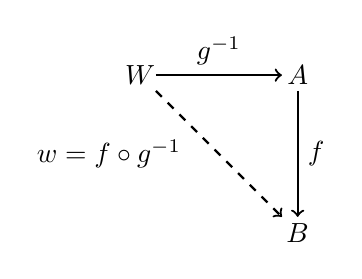
\begin{tikzpicture}
    \draw (0,0) node {$W$};
    \draw (2,0) node {$A$};
    \draw (2,-2) node {$B$};
    \draw[thick, ->] (0.2,0) -- (1.8,0) node[midway, above] {$g^{-1}$};
    \draw[thick, ->] (2,-0.2) -- (2,-1.8) node[midway, right] {$f$};
    \draw[thick, dashed, ->] (0.2,-0.2) -- (1.8,-1.8) node[midway, left=10pt] {$w = f \circ g^{-1}$};
  \end{tikzpicture}
\end{center}

This demonstrates that it is possible to write functions from finite sets to other finite sets, assuming that we can actually write functions like $f$ and $f^{-1}$ in lambda calculus. We begin with the function which takes a set $\{1,\ldots,n\}$ and map them to list of terms of the form $X_1\ldots X_n$.\\

It its simplest form, this function takes elements of the set $\{1,2\}$ and maps them into a list of length 2. We represent $1$ and $2$ with the terms:

\begin{eqnarray*}
  K_2^1 := \l x_1x_2.x_1\\
  K_2^2 := \l x_1x_2.x_2\\
\end{eqnarray*}

So our function consists of a list $\langle X_1,X_2 \rangle$, and takes either of the above functions. In general, we call terms like $\l x_1x_2.x_1$ $K_i^n$, where $n$ is the number of terms in the list, and $i$ is the index of the element we want from inside that list. We can generally define $K_n^i$ as the term\\
\begin{equation*}
  K_n^i := \l x_1\ldots x_n.x_i
\end{equation*}

So now let us say that we have a finite set $\{1,\ldots,n\}$, and we want to create the function $f:\{1,\ldots,n\} \rightarrow \{x_1,\ldots,x_n\}$. Hopefully, we can describe a term $T_f$ such that when we apply it to a term $K_i^n$, it is be beta equal to $K_{f(i)}^n$.
\begin{equation*}
  (T_fK_i^n) =_\beta K_{f(i)}^n
\end{equation*}

This now leaves us with the question of defining $T_f$. An easy way is to simply repeat our table lookup function scheme:
\begin{equation*}
  T_f := \l a.a(K_{f(1)}^nK_{f(2)}^n\ldots K_{f(n)}^n)
\end{equation*}

\examplebox{Example: Demonstration of $T_f$}{
\begin{equation*}
  T_fK_i^n \rightarrow_\beta K_i^n K_{f(1)}^n K_{f(2)}^n \ldots K_{f(n)}^n \twoheadrightarrow_\beta K_{f(i)}^n
\end{equation*}
}

Any function $f:\{1,\ldots,n\} \rightarrow \mathbb{S}$ can be created by this lookup table strategy. But what about functions of the form $f : \{1,\ldots,n\} \times \{1,\ldots,n\} \rightarrow \{1,\ldots,n\}$, or $f(i,j)$? To create functions of more than one variable, we can simply curry the inputs by definining $f_i(j) := f(i,j)$, and redefining $T_f := \l a.aT_{f_1}T_{f_2}\ldots T_{f_n}$.\\

We will defer discussion of the inverse functions until we have a chance to understand techniques for recusion and bounded search. For now, it is sufficient to say that they exist.

\chapter{Lecture 7}
\lhead{January 28, 2015}
\chead{21-366 Lambda Calculus Lecture 7}

\section{Operations on Data Structures}
Now that we have defined some data structures, the next natural step is to perform calculations on them. We establish a number of integer operations, and describe how to use booleans to implement branching. We complete a simple programming environment by describing a strategy for implementing recursion.

\subsection{Integer Addition and Subtraction}
\index{Integer!Integer Addition|textbf}
\index{Integer!Integer Subtraction|textbf}
What is the addition of two integers? Since we represent our integers in the form
\begin{equation*}
  \l xy.\underbrace{xx\ldots x}_{n}y
\end{equation*}
it stands to reason that we want a function $\uline{+}$ such that
\begin{equation*}
  \uline{+}(\l xy.\underbrace{xx\ldots x}_{n}y)(\l xy.\underbrace{xx\ldots x}_{m}y) \twoheadrightarrow_\beta (\l xy.\underbrace{xx\ldots x}_{n + m}y)
\end{equation*}

So our function $\uline{+}$ can simply take one number and insert it into the second. So we can define $\uline{+}$ as:
\begin{equation*}
  \uline{+} := \l uv.\l xy.(ux(vxy))
\end{equation*}
\examplebox{Example: Using $\uline{+}$}{
  \begin{eqnarray*}
    \uline{+}\uline{3}\uline{2} &=_\beta& (\l uv.(\l xy.(ux(vxy))))()()
  \end{eqnarray*}
}

We can see that addition will never result in a number which is not in our set of (nonnegative) integers. A problem arises, however, when we attempt to define subtraction. Defining subtraction as the inverse of addition is unsatisfactory, as many expressions involving subtraction would just not have solutions. To keep subtraction closed on the set of nonnegative integers, we define \textbf{monus subtraction}\index{Monus Subtraction} as
\begin{equation*}
  n \monus m = 0 \hbox{ if } m \geq n \hbox{ else } n - m
\end{equation*}
Monus subtraction is not exactly the integer subtraction that we are used to, but it solves the problem of $A - B$ being undefined whenver $B > A$. In the next lecture, we will explain out how to perform monus subtraction using lambda terms.

Recall our definition of the monus subtraction function:
\begin{equation*}
  n \monus m = \left\{\begin{tabular}{cl}0 & if $m \geq n$\\ $n - m$ & if $m < n$\end{tabular}\right.
\end{equation*}
We can redefine this function in terms of itself, recursively:
\begin{equation*}
  n \monus m = \left\{
  \begin{tabular}{cl}
    $n \monus 0 = n$\\
    $n \monus (m + 1) = $pred$(n \monus m)$\\
  \end{tabular}
  \right.
\end{equation*}


\subsection{Integer Multiplication}
\index{Integer!Integer Multiplication|textbf}
In the last lecture, we introduced methods for representing nonnegative integers, and for adding such integers. A natural next step is to determine a method for computing multiplication. By this point, it should be relatively clear how to proceed.\\

We can define multiplication\index{Multiplication} as
\begin{equation*}
  \uline{\cdot} := \l uv u(\uline{+}v)\uline{0}
\end{equation*}
We have an example:
\begin{equation*}
  \uline{\cdot}\ \uline{n}\ \uline{m} \twoheadrightarrow_{\beta} \uline{n}(\uline{+}\ \uline{m}) \twoheadrightarrow_{\beta} \underbrace{\uline{+}\ \uline{m} (\uline{+}\ \uline{m} ( \ldots (\uline{+}}_{n}\ \uline{m}\ \uline{0}) \ldots ) \twoheadrightarrow_{\beta} \uline{n \cdot m}
\end{equation*}
There exists a simpler, alterantive definition:
\begin{equation*}
  \uline{\otimes} := \l uv . u(vx)
\end{equation*}

Again we compute an example for clarity:
\begin{equation*}
  \uline{\otimes} \uline{n}\ \uline{m} \twoheadrightarrow_{\beta} \l x (\ \uline{n}\ (\uline{m}\ x)) \twoheadrightarrow_{\beta} (\l x \l w \underbrace{(\ \uline{m}\ x(\ldots (\ \uline{m}}_{n}\ x w))))
\end{equation*}
This gives us $n$ nested redexes of the form $\l yx(\ldots(xy)\ldots)(\ \uline{\ \ \ }\ )$

\subsection{The Conditional}
\index{Conditional}
We now return to our definition of the boolean. Recall that we want to use boolean values to determine which branch to take in a conditional statement. In general, we want $\supset KXY =_\beta X$ and $\supset K_*XY =_\beta Y$ for some definition of $\supset$, which we call the conditional. You might notice now that we have done something sneaky. Let us reduce the expression $KXY$.\\

\examplebox{Reduction of $KXY$}{
  \begin{equation*}
    KXY =_\beta (\l xy.x)(XY) \rightarrow_\beta X
  \end{equation*}
}

Huh. It turns out that we can simply use the identity term, $I$, as our conditional. Why do we need the conditional operator at all, then? The answer is that there is more than one way that we can represent $K$ and $K_*$, and not every way that we choose reduces as nicely. Much later, we will find it useful to retain the same structure for terms which we expect to do similar things, so that we can more easily prove that they actually are related.

\subsection{Basic Boolean Operators}
\index{Boolean Operator}
Now that we can branch on individual booleans, we can consider cases where we want to condition on some logical combination of multiple boolean values. To do this, we can implement the basic building blocks of Boolean algebra.\\
\margnot{Boolean Algebra}{ Boolean Algebra was invented by George Boole\index{Boole, George}, a philosopher and logician, for use in determing the truth or falsity of statements.}

There are three main operators which we should implement. The AND operator, the OR operator, and the NOT operator. In computer engineering, these operators are called \textbf{logic gates}\index{Logic Gate}. In logic, they are called \textbf{logical connectives}\index{Logical Connective}. We can think of them as functions of the form $f: B \times B \rightarrow B$, where $B$ is the set $\{1,0\}$ of boolean values.\\

We can easily define the functions in terms of \textbf{truth tables}\index{Truth Table}, which are simply a way of enumerating all possible inputs to a boolean function, and listing their output. Conventionally, we notate the inputs to the function with capital letters starting with 'A', and notate the output with the letter 'S'. True is $1$ and $0$ is false. The truth tables for our three operators are as follows.

\begin{center}
\begin{tabular}{c c | c}
  \multicolumn{3}{c}{AND}\\
  A & B & S\\
  \hline
  \rowcolor{txtbkpaleblue}
  0 & 0 & 0\\
  0 & 1 & 0\\
  \rowcolor{txtbkpaleblue}
  1 & 0 & 0\\
  1 & 1 & 1\\
\end{tabular}
\hspace{1in}
\begin{tabular}{c c | c}
  \multicolumn{3}{c}{OR}\\
  A & B & S\\
  \hline
  \rowcolor{txtbkpaleblue}
  0 & 0 & 0\\
  0 & 1 & 1\\
  \rowcolor{txtbkpaleblue}
  1 & 0 & 1\\
  1 & 1 & 1\\
\end{tabular}
\hspace{1in}
\begin{tabular}{c | c}
  \multicolumn{2}{c}{NOT}\\
  A & S\\
  \hline
  \rowcolor{txtbkpaleblue}
  0 & 1\\
  1 & 0\\
  \multicolumn{2}{c}{}\\
  \multicolumn{2}{c}{}\\
\end{tabular}
\end{center}
Note that these definitions are essentially similar to the English language meanings of the words and, or, and not. Take the statement: ``we need to buy eggs and we need to buy milk.'' If we do not buy both eggs and milk, we have failed in our task.\\

Our simplest operator is NOT. Whenever the input to NOT is true, the output to NOT is false, and vice versa. This can be implemented in lambda calculus as:
\begin{equation*}
  \l b.\supset b K_* K
\end{equation*}
We can demonstrate the correctness of this expression by exhaustive testing. As an aside, this is a good, simple example of the technique presented in the section about finite sets for constructing functions from a lookup table.
\examplebox{Proof of Correctness for NOT}{
  \begin{eqnarray*}
    \hbox{NOT}K &=_\beta& (\l b.\supset bK_*K)K \rightarrow_\beta \supset K K_* K \rightarrow_\beta (\l xy.x)(K_*K) \rightarrow_\beta K_*\\
    \hbox{NOT}K_* &=_\beta& (\l b.\supset bK_*K) \rightarrow_\beta \supset K_* K_* K \rightarrow_\beta (\l xy.y)(K_*K) \rightarrow_\beta K\\
  \end{eqnarray*}
}
We now present the implementations and correctness proofs for AND and OR. Understanding these types of reductions is good practice. Producing these correctness proofs on your own is a good, if quick exercise. These reductions are more explict than strictly necessary, to allow readers who have fallen behind a chance to catch up.
\examplebox{AND and OR}{
  \begin{eqnarray*}
    \hbox{AND}b_1b_2 &:=& \l b_1b_2.\supset b_1b_2 K_*\\
    \hbox{OR}b_1b_2 &:=& \l b_1b_2.b_1 K b_2
  \end{eqnarray*}
}
\examplebox{Proof of Correctness for AND and OR}{
  \begin{eqnarray*}
    \hbox{AND}KK     &=_\beta& (\l b_1b_2.\supset b_1b_2 K_*)KK \rightarrow_\beta \supset KKK_* \rightarrow_\beta (\l xy.x)KK_* \rightarrow_\beta K\\
    \hbox{AND}KK_*   &=_\beta& (\l b_1b_2.\supset b_1b_2 K_*)KK_* \rightarrow_\beta \supset KK_*K_* \rightarrow_\beta (\l xy.x)K_*K_* \rightarrow_\beta K_*\\
    \hbox{AND}K_*K   &=_\beta& (\l b_1b_2.\supset b_1b_2 K_*)K_*K \rightarrow_\beta \supset K_*KK_* \rightarrow_\beta (\l xy.y)KK_* \rightarrow_\beta K_*\\
    \hbox{AND}K_*K_* &=_\beta& (\l b_1b_2.\supset b_1b_2 K_*)K_*K_* \rightarrow_\beta \supset K_*K_*K_* \rightarrow_\beta (\l xy.y)K_*K_* \rightarrow_\beta K_*
  \end{eqnarray*}
  \vspace{.2in}
  \begin{eqnarray*}
    \hbox{OR}KK     &=_\beta& (\l b_1b_2.\supset b_1 K b_2)KK \rightarrow_\beta \supset KKK \rightarrow_\beta (\l xy.x)KK \rightarrow_\beta K\\
    \hbox{OR}KK_*   &=_\beta& (\l b_1b_2.\supset b_1 K b_2)KK_* \rightarrow_\beta \supset KKK_* \rightarrow_\beta (\l xy.x)KK_* \rightarrow_\beta K\\
    \hbox{OR}K_*K   &=_\beta& (\l b_1b_2.\supset b_1 K b_2)K_*K \rightarrow_\beta \supset K_*KK \rightarrow_\beta (\l xy.y)KK \rightarrow_\beta K\\
    \hbox{OR}K_*K_* &=_\beta& (\l b_1b_2.\supset b_1 K b_2)K_*K_* \rightarrow_\beta \supset K_*KK_* \rightarrow_\beta (\l xy.y)KK_* \rightarrow_\beta K_*
  \end{eqnarray*}
}

\section{Recursion}
\index{Recursion|textbf}
Remark: The $1^{\hbox{\footnotesize st}}$ definition of $\uline{\cdot}$ gives us an idea for doing recursion. Given any term $F$ we can iterate $F$ $T$ times as follows:
\begin{eqnarray*}
  F^+ := \l x.xFT\\
  \hbox{then}\\
  F^+\uline{n} \twoheadrightarrow_{\beta} (\underbrace{F(\ldots(F}_{n}T))\ldots)
\end{eqnarray*}
We can do better. We can define a more advanced form of recursion on integers:
\begin{equation*}
  F^+\uline{n + 1}T =_\beta F(F^+\uline{n})T
\end{equation*}
Note that
\begin{equation*}
  F^+\uline{0}T =_\beta T
\end{equation*}
To make this work, we need an auxiliary function $\mathbb{N} \rightarrow$Booleans. We define the sign function\index{Sign Function} and its converse as
\begin{equation*}
  sg(n) = \left\{
  \begin{tabular}{cl}
    TRUE & $n \neq 0$\\
    FALSE & $n = 0$\\
  \end{tabular}
  \right.
  \hspace{1in}
  \uline{\overline{sg}}(n) = \left\{
  \begin{tabular}{cl}
    FALSE& $n \neq 0$\\
    TRUE & $n = 0$\\
  \end{tabular}
  \right.
\end{equation*}
Now we define these functions as lambda expressions:
\begin{eqnarray*}
  \uline{sg} &:=& \l u . u(KK)K_*\\
  \uline{\overline{sg}} &:=& \l u . u(K_*K_*)K\\
\end{eqnarray*}
We observe that this as well works:
\begin{equation*}
  \uline{sg}\ \uline{n} \rightarrow_\beta \uline{n}\ (KK)K_* \twoheadrightarrow_{\beta} \underbrace{(KK)(\ldots}_{n}(KK)K_*)\ldots) \twoheadrightarrow_\beta K
\end{equation*}

\subsection{Computing Predecessor}
\index{Predecessor Function}
Start with two stacks of $1$'s: $0,0$. Assume that at stage $t$ we have $t,$pred$(t)$. At stage $t + 1$, we have $t + 1, t$. After $n$ iterations, you have $n,$pred$(n)$.\\

Here is another method. Represent pred by \uline{pred}. We need a two stack data structure:
\begin{equation*}
  \l a . a\ \uline{n}\ \uline{m}
\end{equation*}
We initialize this structure as $\l a.0\ 0$. We then want to apply some sort of operation to this data structure $u$ times:
\begin{equation*}
  \l u . u\ \boxed{\hphantom{Oh, god}}\ (\l a . a\ \uline{0}\ \uline{0}\ )
\end{equation*}
But what function are we applying in the box?
\begin{equation*}
  \boxed{\hphantom{Oh, god}} := \l z . (\l b . b (\uline{s}\ (zk))(zk))k_*
\end{equation*}
Now we apply it:
\begin{equation*}
  \uline{\hbox{pred}}\ \uline{n}\ \rightarrow_\beta \uline{n}\ (\l z (\l b . b(\uline{s}\ (zk))(zk)))(\l a . a\ \uline{0}\ \uline{0})
\end{equation*}
Notice now that we can simulate a $2$ register machine.\\

\textbf{Remark:} $\uline{\otimes} : \l uv\l x . u(vx) = B$. The $B$ stands for ``beweis,'' which is German for ``proof.'' Now let us take $BFG \twoheadrightarrow_\beta \l x\ (F(Gx))$, or $(BFG)x \twoheadrightarrow_\beta F(Gx)$. Notice that $B$ is a combinator.

\section{Combinators}
\index{Combinator}
$S$ stands for ``substitution.'' $C$ stands for ``commute.''
\begin{eqnarray*}
  I &:=& \l x . x\\
  K &:=& \l xy . x\\
  K^* &:=& \l xy . y\\
  S &:=& \l xyz . xy(yz)\\
  B &:=& \l xyz . x(yz)\\
  C &:=& \l xyz . xzy\\
\end{eqnarray*}
But now we want a combinator which does this:
\begin{equation*}
  \l x \l y_1 \ldots y_n . x y_{\pi(1)} \ldots y_{\pi(n)}
\end{equation*}
where $\pi$ is a permutation on $\{1,\ldots,n\}$.\\

We define one last combinator which, given a function $f: \mathbb{N}^2 \rightarrow \mathbb{N}$ gives a function $f^W(n) = f(n,n)$. This function diagonalizes across the naturals.
\begin{equation*}
  W := \l x \l y \ xyy
\end{equation*}
\chapter{Lecture 8}
\lhead{January 30, 2015}
\chead{21-366 Lambda Calculus Lecture 8}
\pagestyle{fancy}

% TODO: EXPLICITLY DEFINE PUSH
\section{Lists}
\index{List|textbf}
The next data structure which we should construct is the list. Intuitively, it seems as though we should just be able to write out a set of lambda terms one after another, and call that a list. This intuition is not far off. We define the structure of a list as:
\begin{equation*}
  \langle X_1,\ldots,X_n\rangle = \l a. aX_1\ldots X_n
\end{equation*}
To be able to construct lists within lambda calculus, we can define an operator $C_*$ which takes a term to its list. As before, we are using the convention that for some term $X$, $X_* := XI$.
\begin{equation*}
  C_* := (\l cba.(cab))I
\end{equation*}

\examplebox{Demonstration of $C_*$}{
  \begin{eqnarray*}
    C_*X &=_\beta& (\l cba.(cab))IX \rightarrow_\beta \l ba.(Iab)X \rightarrow_\beta \l a.aX
  \end{eqnarray*}
}

\subsection{Concatenation}
\index{List!List Concatenation!textbf}
Now that we have a method for constructing lists of length $1$, we can use them to construct lists with greater length. We can think of the list of two elements as two one-element lists joined together. This joining process is called \textbf{concatenation}. We write the concatenation of two lists $X$ and $Y$ as $X \concat Y$. We can repeat this concatenation process multiple times to build up lists of arbitrary length.\\

We can use this idea of list concatenation on our list structure by defining a combinator which can take the elements of one list and append them to the second. As it turns out, the combinator $B$ does this.\\
\examplebox{$B$ as the list concatenation combinator}{
  Let $\alpha$ and $\beta$ be lists of the form $\alpha = \l a.a\alpha_1,\ldots,\alpha_n = \langle \alpha_1,\ldots,\alpha_n \rangle$ and $\beta = \l a.a\beta_1\ldots\beta_m = \langle \beta_1,\ldots,\beta_m \rangle$.
  \begin{eqnarray*}
    B\alpha\beta &=_\beta& \l xyz.x(yz)\alpha,\beta \rightarrow_\beta \l z.\alpha(\beta z)\\
    &=_\beta& \l z. (\l a.a(\alpha_1\ldots\alpha_n))((\l a.a(\beta_1\ldots\beta_m))z)\\
    &\rightarrow_\beta& \l z.(\l a.a(\alpha_1\ldots\alpha_n))(z(\beta_1\ldots\beta_m))\\
    &\rightarrow_\beta& \l z.z(\beta_1\ldots\beta_m\alpha_1\ldots\alpha_n)
  \end{eqnarray*}
}

One seeming problem with this scheme is that while we defined $\langle X_1\ldots X_n \rangle \concat \langle Y_1\ldots Y_m \rangle$ as $\langle X_1 \ldots X_n Y_1 \ldots Y_m \rangle$, when we converted into lambda terms, we ended up with

\begin{equation*}
  B\langle X_1 \ldots X_n \rangle\langle Y_1 \ldots Y_m \rangle = \langle Y_1 \ldots Y_m X_1 \ldots X_n\rangle.
\end{equation*}

This looks backwards! The key word, however, is ``looks.'' Our notation here is slightly misleading. We have written lists of the form $\langle X_1 \ldots X_n \rangle$ interchangeably with lists of the form $\l a.aX_1\ldots X_n$, but if you construct a list entirely by concatenating lists of length one, you will notice that they are constructed backwards, as $\l a.aX_n \ldots X_1$.\\

\examplebox{Example: Constructing a List}{
  \begin{eqnarray*}
    \langle XYZ \rangle &=& \langle X \rangle \concat \langle Y \rangle \concat \langle Z \rangle = B((B(C_*X)(C_*Y))C_*Z)\\
    &\twoheadrightarrow_\beta& B((\l a.aYX)C_*Z) \twoheadrightarrow_\beta \l a.a ZYX
  \end{eqnarray*}
}

Since the order that a list is written on the page is really just a convention, the inversion of the convention does not affect anything substative, other than allowing us to use $B$ for concatenation instead of a more complicated combinator.

\subsection{Length: An Inefficient Approach}
\margnot{Heads and Tails}{ We call the first element of a list its \textbf{head} and the second element its \textbf{tail}.}
This convention allows us to easily access the last element of a list. We can simply use a combinator like $K$ to ake the first term from the list and project away the rest. But what happens if we want to access the first element?\\

 If we know that the length of the list is $n$, we can just remove the tail of the list $n$ times until we are left with the first element. If we do not know the length, however, this is not possible. So one option is that we could define a new list data structure which somehow encodes its length, perhaps like this: $\langle n \langle X_1,\ldots,X_n\rangle \rangle$.\\

The problem with this is that it is complicated. To concatenate two lists we would have to remove their lengths, add them together, concatenate the lists, and then concatenate on the new length. We could no longer use combinators like $C_*$ and $B$. A better approach will be discussed after we develop fixed point combinators.

\section{Stacks}
\index{Stack|textbf}
Another way to solve the problem of needing list length is to introduce a new data structure: the stack. We define first the empty stack as $E$, and the stack with one element $X_1$ as $\l a . a X_1 E$. If $L$ is a stack of length $n$, then we can create a stack of length $n + 1$ by we simply create a new list $\langle X_{n+1},L\rangle  = \l a\ aX_{n+1}L$. If we expand this list, we get:
\begin{equation*}
  \l a\ aX_{n+1}(\l a\ aX_n(\l a\ aX_{n-1}(\ldots(\l a\ aX_1E)\ldots)))
\end{equation*}
We call this operation ``push.''\index{Push} Analogously we define a ``pop''\index{Pop} operation and a ``tail''\index{Tail} operation as
\begin{eqnarray*}
  \langle X_{n+1},L \rangle K &=_\beta& X_{n+1}\\
  \langle X_{n+1},L \rangle K_* &=_\beta& L\\
\end{eqnarray*}
But what happens if we attempt to pop from an empty list? We need to test for an empty list. Our test should take a list and if it is nonempty, return a $K$. We can do this with a test:
\begin{equation*}
  TEST: \l u\ u(\l zwv.K)(\l ab.K_*)
\end{equation*}
To make this happen, we can define $E = \l ab.K_*$.\\

To confirm that this works, we will test on the list $<X,L>$.
\begin{eqnarray*}
  TEST\langle X,L\rangle &\rightarrow_\beta& \langle X,L\rangle (\l zwv.K)(\l ab.K_*) \rightarrow_\beta (\l zwv.K)XL(\l ab.K_*) \twoheadrightarrow_\beta K\\
  TEST\ E &\twoheadrightarrow_\beta& E(\l xwv.K)(\l ab.K_*) \twoheadrightarrow_\beta K_*\\
\end{eqnarray*}

\section{Unbounded Search}
\index{Unbounded Search|textbf}
How do we search for a number? For example, say that we want to find a prime number in the list of natural numbers. In general, we write that we are looking for an $n$ such that $\Phi(n)$ is true. We can see a pattern of cases:
\begin{eqnarray*}
  \Phi(0) \rightarrow 0\\
  ~\Phi(0), \Phi(1) \rightarrow 1\\
  ~\Phi(0), ~\Phi(1), \Phi(2) \rightarrow 2\\
  \ldots
\end{eqnarray*}
More generally, we can define a function:
\begin{equation*}
  f(x) = \left\{
  \begin{tabular}{c l}
    $n$ & if $\Phi(n)$\\
    $f(n + 1)$ & otherwise\\
  \end{tabular}
  \right.
\end{equation*}

\subsection{G\"odel's Fixed Point Theorem}
\index{Godel's Fixed Point Theorem@G\"odel's Fixed Point Theorem}
G\"odel's Fixed Point Theorem asserts that 

If a term $T$ has a fixed point $F$ such that $(TF) =_\beta F$, then $F$ in some way has to depend on self application, as the statement $\exists F \mid (TF) =_\beta F$ is not true in general for all $T$. This implies that $T(XX) = XX$. We can write:
\begin{eqnarray*}
  T(XX) &=& (XX)\\
  (\l xT(XX))X &=& (XX)\\
  X &=& \l x\ T(XX)\\
  (\l x\ T(XX))(\l x\ T(XX)) &=_\beta& T((\l x\ T(XX))(\l x\ T(XX))\\
  X &=_\beta& TX\\
\end{eqnarray*}
We define this as Curry's Paradoxical Combinator\index{Curry, Haskell!Curry's Paradoxical Combinator}. It is a fixed point combinator.
\begin{equation*}
  Y_{Curry} := \l y\ (\l x\ (y(xx)))(\l x.y(xx)) 
\end{equation*}
We can apply $Y_{Curry}$ to $T$.
\begin{eqnarray*}
  Y_{Curry}T \rightarrow_\beta (\l x\ T(xx))(\l x\ T(xx))\\
  \rightarrow_\beta T((\l x\ T(xx))(\l x\ T(xx))) \leftarrow_\beta T(Y_{Curry}T)
\end{eqnarray*}
We can define as well Turing's Fixed Point Combinator\index{Turing's Fixed Point Combinator}:
\begin{equation*}
  Y_{Turing} = \underbrace{(\l xy . y(xxy))}_{\alpha}\underbrace{(\l xy . y(xxy))}_{\alpha}
\end{equation*}
What happens when we apply $Y_{Turing}$ to $T$?
\begin{eqnarray*}
  Y_{Turing}T \rightarrow_\beta (\l y\ y(\alpha\alpha y))T \rightarrow_\beta T(\alpha\alpha T)
\end{eqnarray*}
It turns out that $Y_{Turing}$ is much more useful, but $Y_{Curry}$ is easier to determine.

\section{* Practical Uses for $Y$, the Fixed Point Combinator}
One problem which arises from our current construction of $\l$ calculus is that we do not have a mechanism for recursion. When we usually think of recursion\index{Recursion}, we think of it as a function which calls itself. This is not possible yet. Notice that we would need some way of referring to a function from inside itself. We can do this by passing a function to itself as an argument. $Y$ allows us to evaluate an expression with itself as an argument. Remember that
\begin{center}
  Y\ g $\twoheadrightarrow_\beta$ g\ (Y\ g)
\end{center}
By repeatedly applying this $\beta$ reduction, we can have $g$ applied to itself as many times as we want.\\

Take, for example, a function for computing the factorial of a number, \uline{fac}. In pseudocode, we can implement \uline{fac} tail recursively\index{Tail Recursion} as
\begin{lstlisting}[language=Python]
  def fac(n):
     if (n == 1):
        1
     else:
        n * fac(n - 1)
\end{lstlisting}
% TODO: finish this explanation, based on http://www.righto.com/2009/03/y-combinator-in-arc-and-java.html
\chapter{Lecture 9}
\lhead{February 2, 2015}
\chead{21-366 Lambda Calculus Lecture 9}
\rhead{Brian Jacobs}
\pagestyle{fancy}

\section{Lists of Integers}
\index{List!of Integers}\index{Integer}
Our goal now is to find the length of a list of integers.\\
Recall that:
\begin{eqnarray*}
  Y_{Curry} = \l y((\l x\ y(xx))(\l x\ y(xx)))\\
  Y_{Turing} = (\l xy . y(xxy))(\l xy . y(xxy))\\
\end{eqnarray*}
\begin{eqnarray*}
  \langle x_1,\ldots,x_n \rangle &=& \l a . aX_1\ldots X_n\\
  \hbox{length}(\langle x_1,\ldots,x_n \rangle ) &=& n\\
\end{eqnarray*}
If we take our representation of nonnegative integers, and define a new encoding such that $n = n' + 1$, we can get a representation of nonnegative integers using only positive integers. This leaves us with zero as a special value, which we can use to mark the end of a list. We can then encode a list of nonnegative integers $m_1,m_2,\ldots,m_n$ as $m_1+1,m_2+1,\ldots,m_n+1,0$.\\

\begin{equation*}
  \l a . a\ \uline{m_1+1}\ \ldots\ \uline{m_n+1}\ \uline{0}
\end{equation*}
We compute the length function $f$.
\begin{equation*}
  Y_{Turing}(\underbrace{\l f \l xy. (\uline{sg}\ y)(f(\uline{s}x))x}_{L})\uline{0}
\end{equation*}
So we take $C_*(Y_{Turing}L)$ to cause application to a list to put the list in function position:
\begin{equation*}
  C_*(Y_{Turing}L\uline{0})(\l a . a(\uline{m_1+1}\ \ldots \uline{m_n+1}, \uline{0})) \rightarrow_\beta (\l a . a(\uline{m_1+1}\ \ldots \uline{m_n+1}, \uline{0}))(Y_{Turing}L\uline{0})
\end{equation*}
\subsection{Computing the Maximum of a List}
Imagine that you are in a pumpkin patch with your children, who want the largest pumpkin possible with which to make a jack-o-lantern. You start down the first row of pumpkins, and look at the first one. ``This is the largest pumpkin I have seen yet!'' you say. So you take it with you. The next several pumpkins are all smaller than the one you are carrying, so you pass them by.\\

Eventually you come to a 

\subsection{Testing our list length function}
\begin{eqnarray*}
  (Y_{Turing}L\uline{0} \uline{m_1+1})\\
  \ldots % TODO: finish beta reduction to the length
\end{eqnarray*}

\section{Simultaneous Fixed Points}
\index{Fixed Point|textbf}
There are more kinds of fixed points, other than the ones found by Turing and Curry. We defined a simple fixed point\index{Fixed Point!Simple Fixed Point} as
\begin{equation*}
  Ff =_\beta f
\end{equation*}
We can define simultaneous fixed points\index{Fixed Point!Simultaneous Fixed Point} as
\begin{eqnarray*}
  f = Ffg = F(\langle f,g\rangle K)(\langle f,g \rangle K_*)\\
  g = Gfg = G(\langle f,g\rangle K_*)(\langle f,g\rangle K_*)\\
\end{eqnarray*}
We can see that
\begin{equation*}
  \langle f,g\rangle = \l x\ \langle F(\langle f,g\rangle ,K)(\langle f,g\rangle K_*),G(\langle f,g\rangle ,K)(\langle f,g\rangle K_*)\rangle \langle f,g\rangle
\end{equation*}
So, we can set
\begin{equation*}
  f = \underbrace{Y_{Turing} (\l x \langle F(xK)(xK_*),G(xK)(xK_*)\rangle )}_{\alpha}K
\end{equation*}
and
\begin{equation*}
  g = Y_{Turing} (\l x \langle F(xK)(xK_*),G(xK)(xK_*)\rangle)K_*
\end{equation*}
We can apply
\begin{eqnarray*}
  \l x \langle F(\langle f,g\rangle,K)(\langle f,g\rangle K_*),G(\langle f,g\rangle,K)(\langle f,g\rangle K_*)> \alpha = \langle F(\alpha K,\alpha K_*), G(\alpha K, \alpha K_*)\rangle &K& = f\\
&K_*& = g
\end{eqnarray*}

Let $f = Ffg$ and $g = Gfg$. We will define $\Phi(g) = F(\Phi g)g$. If we take $\alpha = Y_{Turing}(\l xy . F(xy)y)$. What do we know about $\alpha$? $\alpha = \Phi = \l y\ F(\Phi y,y)$.\\

What:
\begin{equation*}
  Y_{Turing} (\l y G(F(Y_{Turing}(\l uv.F(uv)v)y)y)y)
\end{equation*}

\section{The SKI Combinator Calculus}
\index{SKI Combinator Calculus|textbf}
\subsection{Closing Terms with Bracket Abstraction}
It seems like it should not be too difficult to take an open expression and convert it into one which is closed. One process which accomplishes this is called \textbf{bracket abstraction}\index{Bracket Abstraction|textbf}. Let $x,y$ be variables. We recursively define bracket abstraction as:
\begin{eqnarray*}
  {[x]}y &:=& Ky\\
  {[x]}x &:=& I\\
  {[x]}(E_1,E_2) &:=& S([x]E_1)([x]E_2)
\end{eqnarray*}

We claim two things about the bracket abstraction: first, that if $U$ is an applicative combination of $S,K,I$ and free variables, then $([x]U)x \twoheadrightarrow_\beta U$, and second, that the bracket abstraction of an open term $U$ is closed.\\

We can prove our first claim inductively. Let our bracket abstraction be $[x]U$. Our base case is where $U$ is a free variable. There are then two possible subcases depending on whether $U = x$ or $U \neq x$. If $U = x$, then our bracket abstraction is $[x]x = I$, and our claim holds: $Ix \rightarrow_\beta x$. If $U = y \neq x$, then we have $[x]y = Ky$, and we have $Kyx \rightarrow_\beta y$.\\

This leaves our inductive step, where $U = QV$. $[x]U$ is therefore $S([x]Q)([x]V)$. By our induction hypothesis, $[x]Qx \rightarrow_\beta Q$ and $[x]Vx \rightarrow_\beta V$. We can perform a $\beta$ reduction to get
\begin{equation*}
  S([x]Q)([x]V)x \twoheadrightarrow_\beta [x]Qx([x]Vx) \twoheadrightarrow_\beta QV
\end{equation*}

Our second claim can also be proven inductively. We again use the bracket abstraction $[x]U$. Our base case is again that $U$ is a free variable. If $U = x$, then we get $[x]x = I$, which is closed. If $U = y$, then we get $[x]y = Ky =_\beta \l x.y$, which is closed. In our inductive step, we assume by our induction hypothesis that $[x]Q$ and $[x]V$ are closed, and we apply
\begin{equation*}
  S([x]Q)([x]V) =_\beta \l xyz.([x]Q)([x]V) \rightarrow_\beta \l z.([x]Qz)([x]Vz)
\end{equation*}

This is a closed term as well. When taken together, we can see that the bracket abstraction is a transformation which allows us to close open terms without altering their meaning.

\subsection{Church and Curry's Combinator Calculii}
How many combinators do we really need? At this juncture, we have defined a moderately sizeable list of combinators to perform a variety of tasks. As it turns out, we can construct some of these combinators out of more simple ones. In fact, every closed term in the lambda calculus can be represented with nothing more than the combinators $S,K$ and $I$. This claim is was made by Curry, and the resulting system is called the SKI combinatory logic. There is a weaker version of this theorem which was proven by Church that relies on the combinators $B,C,K,W,$ and $I$. We will prove Curry's version.\\

\examplebox{Recall: $S, K$, and $I$}{
  \begin{eqnarray*}
    S &:=& \l xyz.xz(yz)\\
    K &:=& \l xy.x\\
    I &:=& \l x.x\\
  \end{eqnarray*}
}

\subsection{Proof of Completeness for SKI}
We prove that any lambda term can be written using only $S,K$ and $I$ by introducing a transformation $T[X] = Y$ which takes an arbitrary lambda term $X$ and converts it into an applicative combination of $S,K$ and $I$ with free variables. $T[\ ]$ is defined recursively as follows.
\begin{eqnarray*}
  T[x] &:=& x\\
  T[(XY)] &:=& (T[X] T[Y])\\
  T[\l x.X] &:=& (K T[X])\hbox{ if $x \not\in \FV(X)$}\\
  T[\l x.x] &:=& I\\
  T[\l xy.E] &:=& T[\l x.T[\l y.E]]\hbox{ if $x \in \FV(E)$}\\
  T[\l x.(XY)] &:=& (S T[\l x.X] T[\l x.Y])\hbox{ if $x \in \FV(X)$ or $x \in \FV(Y)$}
\end{eqnarray*}

As should now be familiar, our proof will proceed by induction on the structure of a lambda term, $U$. In our base case, $U = x$ and $T[x] = x$. For our inductive step, we have our usual two cases. For our first case, consider $U = (XY)$. Since $T[(XY)] = (T[X]T[Y])$, and we know that $T[X]$ and $T[Y]$ are applicative combinations of $S,K,I$ and free variables, the application $(T[X]T[Y])$ is also in SKI.\\

Finally, we have the case where $U = \l x.V$, which breaks down into several further subcases. If $V = x$, then we simply have the identity combinator, $I$. If $V = X$ and $x$ is not in the free variables of $X$, then $T[\l x.X] = KT[X]$

% http://en.wikipedia.org/wiki/Combinatory_logic#Completeness_of_the_S-K_basis

\subsection{Proof of Equivalence for $T[\ ]$}

\section{Yet Smaller: The $\iota$ Combinatory Logic}
If our objective is minimalism, we can do better than SKI combinatory logic by observing that there exists a combinator which can be used to construct the SKI combinators. This combinator was discovered by Chris Barker, and is called $\iota$.

\begin{eqnarray*}
  \iota x &:=& \l x.(xS)K\\
\end{eqnarray*}

Applying $\iota$ to itself gives us the identity combinator, $I$.\\

\examplebox{Deriving $I$ from $\iota$}{
  \begin{eqnarray*}
    \iota\iota &=_\beta& (\l x.(xS)K)\iota \rbeta (\iota S)K\\
    &=_\beta& ((\l x.(xS)K)S)K \rbeta ((SS)K)K)\\
    &=_\beta& ((((\l xyz.(xz)yz)S)K)K) \rbeta ((SK)KK)\\
    &=_\beta& ((\l xyz.(xz)yz)(K))(KK) \rbeta \l z.(Kz)(KK)\\
    &=_\beta& \l z.(\l xy.x)z(KK) \rbeta \l z.z\\
    &=_\beta& I
  \end{eqnarray*}
}

If we apply $\iota$ twice to $I = \iota\iota$ we get $K$.\\

\examplebox{Deriving $K$ from $\iota$ and $I$}{
  \begin{eqnarray*}
    \iota\iota I &=_\beta& \iota((\l x.(xS)K) I) \rbeta \iota((IS)K) \rbeta \iota(SK)\\
    &=_\beta& (\l x.(xS)K)(SK) \rbeta (SK)SK\\
    &=_\beta& KK(SK) =_\beta K
  \end{eqnarray*}
}

Applying $\iota$ one more time gives us $S$.\\

\examplebox{Deriving $S$ from $\iota$ and $K$}{
  \begin{eqnarray*}
    \iota K &=_\beta& (\l x.(xS)K) \rbeta (KS)K \rbeta S
  \end{eqnarray*}
}
\chapter{Lecture 10}
\lhead{February 4, 2015}
\chead{21-366 Lambda Calculus Lecture 10}
\rhead{Brian Jacobs}
\pagestyle{fancy}

\section{A Review}
\subsection{Combinators}
\begin{eqnarray*}
  B &:=& \l xyz . x(yz)\\
  C &:=& \l xyz . xzy\\
  K &:=& \l xy . x\\
  I &:=& \l x .x\\
  W &:=& \l xy . xyy\\
  S &:=& \l xyz . xz(yz)
\end{eqnarray*}
\subsection{Bracket Abstraction}
\index{Bracket Abstraction|textbf}
\begin{equation*}
  [x] \left\{
  \begin{tabular}{c}
    S\\K\\I\\y
  \end{tabular}
  \right. = \left\{
  \begin{tabular}{l}
   $KS$\\$KK$\\$KI = K_*$\\$Ky$
  \end{tabular}
  \right.
\end{equation*}
\begin{equation*}
  [x](XY) = S([x]X)([x]Y), [x]x = I
\end{equation*}
$[x]X$ is defined for $X$ an applicative combinations of $S, K, I$ and variables.\\

\section{Beta Conversion of Terms}
\textbf{Lemma:} $([x]X)x \twoheadrightarrow_\beta x$.\\

\textbf{Proof:} by induction on the definition of bracket abstraction. The base case is $X$ is one of $S,K,I,x$. So, $[x]x := Ix = x$, and we additionally have
\begin{eqnarray*}
  KSx &\rightarrow_\beta& S\\
  KKx &\rightarrow_\beta& K\\
  KIx &\rightarrow_\beta& I\\
\end{eqnarray*}
Remark: We could replace $I$ by $SKK$.
\begin{equation*}
  SKKx \rightarrow_\beta (Kx)(Kx) \rightarrow_\beta x
\end{equation*}
Inductive step: $[x](UV)x$ is by definition $S([x]U)([x]V)x \rightarrow_\beta ([x]Ux)([x]Vx)$. By the induction hypothesis, $[x]Ux \twoheadrightarrow_\beta U$ and $[x]Vx \twoheadrightarrow_\beta V$. \qqed\\

We define for each term $X$ an applicative combination of $S, K,$ and the free variables of $X$ as $X^{CL}$, where the $CL$ stands for Combinatory Logic. It might be better to call it combinatory algebra, but it retains the $CL$ name for historical reasons. Dude who named them (Curry?) thought it could be a foundation for all of mathematics.\\

How do we formally define $X^{CL}$?
\begin{eqnarray*}
  x^{CL} = x\\
  (XY)^{CL} = (X^{CL}Y^{CL})\\
  (\l xX)^{CL} = [x]X^{CL}
\end{eqnarray*}

\textbf{Claim:} $X^{CL} \twoheadrightarrow_\beta X$.\\

\textbf{Proof:} Induction on the definition of $X^{CL}$. Base case: clear. %todo: fix this
Induction step: Case 1: $X = (UV)$. Then $X^{CL} = (U^{CL}V^{CL})$, and by the induction hypothesis, $U^{CL} \twoheadrightarrow_\beta U$ and $V^{CL} \twoheadrightarrow_\beta V$. Case 2: $X = \l uU$. Then $X^{CL} = [u]U$. By induction on $U$, basis case: $U = V \neq u$. Then $[u]U = Kv \rightarrow_\beta \l u.v = \l u.U$. If $U = u$, then $[u]U = I = \l u.u = \l u.U$. Induction step: $U = Z_1Z_2$. $[u]U = [u](Z_1Z_2) = S([u]Z_1)([u]Z_2)$. We have now
\begin{equation*}
  S : \l xyu.(xu)(yu)
\end{equation*}
So $\l u ([u]Z_1u)([u]Z_2u)$ which reduces by our lemma to $\twoheadrightarrow_\beta \l u(Z_1Z_2) = \l u(U)$.\\

Finally, $U = \l vV$. We will leave this case as an exercise. \qqed

\section{Useful Combinators}
\def\arraystretch{1.5}
\begin{tabular}{c c c}
  \multirow{2}{*}{Booleans} & $K := \l xg.x$ & TRUE\\
  & $K_* := \l xy.y$ & FALSE\\
  \cline{2-2}
  & ONE $:= \l abc.a$ & \\
  & TWO $:= \l abc.b$ & \\
  & THREE $:= \l abc.c$ & \\
  \cline{2-2}
  &&\\
  Equality function & $Eq\ \uline{n}\ \uline{m} = \left\{\begin{tabular}{c l}$K$ & if $n = m$\\$K_*$ & if $n \neq m$\end{tabular}\right.$ &\\
  &&\\
\end{tabular}\\

Notice that we should be able to derive $Eq$ if we have a function $E$ such that
\begin{equation*}
  E\ \uline{n}\ \uline{m} = \left\{
  \begin{tabular}{c l}
    $\uline{1}$ & if $n = m$\\
    $\uline{0}$ & if $n \neq m$\\
  \end{tabular}
  \right.
\end{equation*}
We can define a function $E(x,y) := \overline{sg}((x \monus y) + (y \monus x))$, where $sg(0) = 0$ and $sg(n+1) = 1 \forall n \in N$ and $\overline{sg}$ is defined as $\overline{sg} = 1 $ iff $sg = 0$ and $\overline{sg} = 0$ otherwise.

\chapter{Lecture 11}
\lhead{February 6, 2015}
\chead{21-366 Lambda Calculus Lecture 11}
\rhead{Brian Jacobs}
\pagestyle{fancy}

\section{Even More Data Structures}

\subsection{Stacks}
The empty stack is defined as $KK_*$, or THREE. If our stack is $\l a\ aLR$, $L$ is the top, $R$ is the result of popping the stack.

\subsection{Trees}
What will we do today?
\begin{enumerate}[(I)]
  \item Describe the data structure
  \item Tasks:
    \begin{itemize}
      \item insertion of an element
      \item balancing the tree
      \item finding an element in the tree
    \end{itemize}
  \item write an informal algorithm for finding an element in a tree
    \begin{itemize}
      \item write a lambda term which implements our algorithm
    \end{itemize}
\end{enumerate}

A tree is a data structure which is comprised of leaves and internal nodes, where a leaf is defined as an ordered triple $<\hbox{TRUE}, \uline{n}, X>$ of a boolean which is true, an index number, and an object. An internal node is an ordered triple of $<\hbox{FALSE}, L, R>$ of a false boolean, a left subtree, and a right subtree.\\

We provide a recursive definition of trees: $<\hbox{TRUE}, \uline{n+1}, X>$ is a tree, and $<\hbox{FALSE}, L, R>$ is a tree.\\

Now we describe our algorithm: $f(x,y,z)$ where $x$ is a tree, $z$ is the item we are searching for, and $y$ is a stack of trees. If $x$ is a leaf, then $x(TWO)$ is the index. We apply $Eq(x(TWO))z$. If this is $\uline{1}$, then we want to return $x$ of 3, so we write:
\begin{equation*}
  Y_{Turing}(x(ONE)(Eq(x(TWO))z(x(THREE))(f\ (\hbox{TOP }y)(\hbox{POP }y)z)(f (x(TWO))(\l a\ a(x(THREE))y))))
\end{equation*}
We call this function as $Fx(\hbox{Empty stack}z)$.\\
\chapter{Lecture 12}
\def\over#1#2{#1}
\def\LeftRightarrow{\Leftarrow\Rightarrow}

\lhead{February 9, 2015}
\chead{21-366 Lambda Calculus Lecture 12}
\pagestyle{fancy}

\section{Untitled on Board}
\begin{equation*}
  ((\l x X)Y) \rightarrow_\beta [Y/x]X
\end{equation*}
Step 1:
\begin{equation*}
  U_1 \rightarrow_\beta \Rightarrow U_1V \rightarrow_\beta U_2V \hbox{ and } VU_1 \rightarrow_\beta VU_2
\end{equation*}
Also,
\begin{equation*}
  \l uU_1 \rightarrow_\beta \l uU_2
\end{equation*}
Many steps:
\begin{eqnarray*}
  U \rightarrow_\beta V \Rightarrow U \twoheadrightarrow_\beta V,\ U = V \Rightarrow U \rightarrow_\beta V.\\
  U_1 \twoheadrightarrow_\beta U_2 \hbox{ and } V_1 \twoheadrightarrow_\beta V_2 \Rightarrow U_1V_1 \twoheadrightarrow_\beta U_2V_2\\
\end{eqnarray*}
Additionally,
\begin{eqnarray*}
  U \twoheadrightarrow_\beta V \Rightarrow \l uU \twoheadrightarrow_\beta \l uV\\
\end{eqnarray*}

\subsection{Reduction Sequence}
\index{Reduction Sequence}
We define a reduction sequence from $U$ to $V$ as a set of $\beta$ reductions $\Delta_i$ such that
\begin{equation*}
  U = U_0 \stackrel{\Delta_0}{\rightarrow_\beta} U_1 \rightarrow_\beta \ldots \stackrel{\Delta_{n-1}}{\rightarrow_\beta} U_n = V
\end{equation*}

$U =_\beta V$ is the smallest equivalence relation\index{Equivalence Relation} $\subseteq \twoheadrightarrow_\beta$. We say that $U =_\beta V \LeftRightarrow$ there exists a sequence of terms $U_0, U_1,\ldots U_{2n}$ such that
\begin{center}
  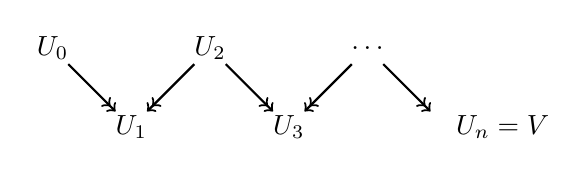
\begin{tikzpicture}
    \draw (0,0) node {$U_0$};
    \draw[->>,thick] (.2,-.2) -- (.8,-.8);
    \draw (1,-1) node {$U_1$};
    \draw[<<-,thick] (1.2,-.8) -- (1.8,-.2);
    \draw (2,0) node {$U_2$};
    \draw[->>,thick] (2.2,-.2) -- (2.8,-.8);
    \draw (3,-1) node {$U_3$};
    \draw[<<-,thick] (3.2,-.8) -- (3.8,-.2);
    \draw (4,0) node {$\ldots$};
    \draw[->>,thick] (4.2,-.2) -- (4.8,-.8);
    \draw (5,-1) node[anchor=west] {$U_{n} = V$};
  \end{tikzpicture}
\end{center}

\section{Church-Rosser Theorem}
\index{Church-Rosser Theorem|textbf}
The Church-Rosser theorem states that if there exists a term $U =_\beta V$ then there exists a $W$ such that $U \twoheadrightarrow_\beta W \twoheadleftarrow_\beta V$. We state it now without proof, but over the course of the next couple of lectures we will build up to a proof.\\

\subsection{Strong Diamond Property}
\index{Diamond Property!Strong Diamond Property|textbf}
The proof of the Church-Rosser theorem establishes something called the ``diamond property.''\index{Diamond Property} The idea is that if we can take a ``hill'' and turn it into a ``valley,'' then we can ``pave'' a sequence of beta reductions into a single valley. Formally, the diamond property states that: if
\begin{equation*}
  U \twoheadleftarrow_\beta X \twoheadrightarrow_\beta V
\end{equation*}
 
\subsection{Notes on Diagrams}
In a diagram, you see both solid lines and dotted lines. The solid lines are read ``if this line exists,'' and the dotted lines are read ``then this line exists.''
\begin{center}
  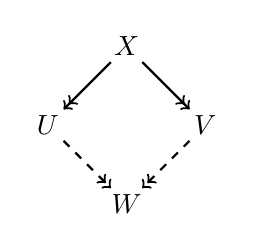
\begin{tikzpicture}
    \draw (0,0) node {$X$};
    \draw[->>,thick] (-.2,-.2) -- (-.8,-.8);
    \draw (-1,-1) node {$U$};
    \draw[dashed,->>,thick] (-.8,-1.2) -- (-.2,-1.8);
    \draw (1,-1) node {$V$};
    \draw[->>,thick] (.2,-.2) -- (.8,-.8);
    \draw (0,-2) node {$W$};
    \draw[dashed,->>,thick] (.8,-1.2) -- (.2,-1.8);
  \end{tikzpicture}
\end{center}

We can attempt to prove the strong diamond property (which is not true.) Imagine that we have $U \over{\Delta_1}{\leftarrow_\beta} X \over{\Delta_2}{\rightarrow_\beta} V$. $\Delta_1$ and $\Delta_2$ are disjoint. Notice that $\Delta_2$ has a unique residual in $U$, and $\Delta_1$ has a unique residual in $V$. We can then do:
\begin{eqnarray*}
  U \stackrel{\Delta_1}{\leftarrow_\beta} D \stackrel{\Delta_2}{\rightarrow_\beta} V\\
  U \stackrel{\Delta_2}{\rightarrow_\beta} D' \stackrel{\Delta_1}{\leftarrow_\beta} V\\
\end{eqnarray*}

Notice that
\begin{equation*}
  [Y_1/x]([Y_2/z]X_2) = [Y_1/x, [Y_1/x]Y_2/z]X
\end{equation*}

Our final case is the degenerate case $\Delta_2$ is in $Y_1$. We then have
\begin{center}
  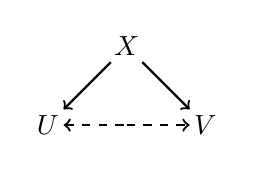
\begin{tikzpicture}
    \draw (0,0) node {$X$};
    \draw (-1,-1) node {$U$};
    \draw (1,-1) node {$V$};
    \draw[thick,->] (-.2,-.2) -- (-.8,-.8);
    \draw[thick,->] (.2,-.2) -- (.8,-.8);
    \draw[thick,dashed,->] (0,-1) -- (.8,-1);
    \draw[thick,dashed,<-] (-.8,-1) -- (0,-1);
  \end{tikzpicture}
\end{center}
So, strong diamond property does not work, but this is okay for the purposes of proving Church-Rosser. At this point in the proof, many people part ways. Church and Rosser have a proof, as do Kleene and J.J. Levy/Hindley.\\

Church and Rosser show that all of the redexes of $\Delta_2$ are disjoint. So eventually we get to our original, nondegenerate case. We will take a different route.\\

\subsection{Weak Diamond Property}
\index{Diamond Property!Weak Diamond Property|textbf}
The weak diamond property replaces the single beta reductions with beta reduction sequences:
\begin{center}
  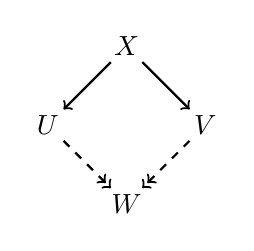
\begin{tikzpicture}
    \draw[thick,->] (-.2,-.2) -- (-.8,-.8);
    \draw[thick,dashed,->>] (-.8,-1.2) -- (-.2,-1.8);
    \draw[thick,->] (.2,-.2) -- (.8,-.8);
    \draw[thick,dashed,->>] (.8,-1.2) -- (.2,-1.8);

    \draw (0,0) node {$X$};
    \draw (-1,-1) node {$U$};
    \draw (1,-1) node {$V$};
    \draw (0,-2) node {$W$};
  \end{tikzpicture}
\end{center}
Unfortunately, the weak diamond property is not enough on its own. We cannot prove Church-Rosser using weak-diamond. Explaining why uses surjective pairings and is beyond the scope of this course.\\

\subsection{A Brief Combinatorial Fact: K\"onig's Lemma}
\index{Konig's Lemma@K\"onig's Lemma|textbf}
The German mathematician K\"onig had a theorem, called K\"onig's Lemma: a finitely branching tree with no infinite path is finite. The contrapositive is that if we have an infinite tree, then we have an infinite path.\\

\textbf{Proof:} Suppose that $T$ is an infinite, finitely branching tree. We find our infinite path in the following way. Consider all the subtrees of $T$: $T_1,\ldots T_n$. By the pidgeonhole principle, at least one of these subtrees must be infinite. Take the edge to that subtree. This finds us an infinite path. \qqed
\chapter{Lecture 13}
\lhead{February 11, 2015}
\chead{21-366 Lambda Calculus Lecture 13}

\section{Normalization}
A question which arises now is how we determine whether two terms are equivalent, for some definition of equivalence. Clearly, for instance, the terms $\l x.X$ and $\l y.X$ share some common structure which the terms $\l xy.X$ and $\l z.Z$ do not. But what do we say about the terms $\l xy.X$ and $X$? Since $\l xy.X \rightarrow_\beta X$, it makes some sort of sense to say that $\l xy.X =_\beta X$ as well. But what about terms with more complicated structure? It is nice, for the purposes of comparison, if we can put terms into some sort of normal form.\\

We say that a term $X$ is \textbf{normal}\index{Normal Term} if it cannot be contracted by $\beta$ reduction. This seems like a natural place to make comparisons from. We have contracted the term as far as we can contract it, and now it cannnot be contracted anymore. Recall that a term is contractable by $\beta$ reduction if it has a $\beta$ redex as a subterm. So we contract all of the $\beta$ redexes to reach normal form. Obviously, this is not possible in all cases; simply consider trying to find a normal form for $\Omega$!\\

$X$ is said to be \textbf{normalizable}\index{Normalizable Term} if there exists a term $N$ in normal form such that $X \twoheadrightarrow_\beta N$. We will eventually prove that this implies some sort of uniqueness about the term $X$. $X$ is said to be \textbf{strong normalizable}\index{Strong Normalizable Term} if every reduction sequence of $X$ ultimately ends in a normal form term. We indicate that $X$ is strongly normalizable by $X \in \hbox{SN}$.\\

To understand why the distinction between normalizable and strong normalizable is necessary, consider the term $Kx\Omega$. There are two possible $\beta$ reductions:
\begin{eqnarray*}
  Kx\Omega &\rightarrow_\beta& x\\
  Kx\Omega &\rightarrow_\beta& Kx(\Omega\Omega)
\end{eqnarray*}
Clearly, one of these reduction sequences terminates in the normal term $x$. The term $Kx(\Omega\Omega)$, however, is in the same situation as $Kx\Omega$. By reducing the $K$ first, we can return to our normal form $x$. However areduction sequence which consists of the repeated reduction of $\Omega$ will never terminate in a normal form. It is worth noting as well that if a reduction sequence of $Kx\Omega$ ever does terminate, it terminates in the form $x$. You might recall that this is simply our weak diamond property.
\begin{center}
  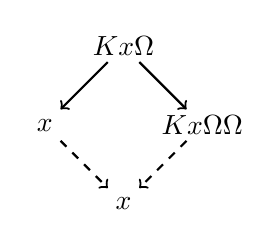
\begin{tikzpicture}
    \draw (0,0) node {$Kx\Omega$};
    \draw (-1,-1) node {$x$};
    \draw (1,-1) node {$Kx\Omega\Omega$};
    \draw (0,-2) node {$x$};
    \draw[thick, ->] (-.2,-.2) -- (-.8,-.8);
    \draw[thick, ->, dashed] (-.8,-1.2) -- (-.2,-1.8);
    \draw[thick, ->] (.2,-.2) -- (.8,-.8);
    \draw[thick, ->, dashed] (.8,-1.2) -- (0.2,-1.8);
  \end{tikzpicture}
\end{center}

\subsection{Reduction Sequences of Strongly Normalizable Terms}
We claim that if $X$ is strongly normalizable, then the entire reduction tree of $X$ is finite, and the tree ends in a unique normal form $W$.
\begin{center}
  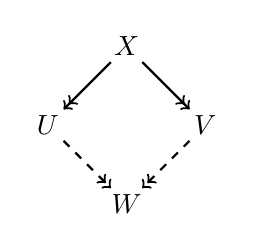
\begin{tikzpicture}
    \draw (0,0) node {$X$};
    \draw (-1,-1) node {$U$};
    \draw (1,-1) node {$V$};
    \draw (0,-2) node {$W$};
    \draw[thick, ->>] (-.2,-.2) -- (-.8,-.8);
    \draw[thick, ->>, dashed] (-.8,-1.2) -- (-.2,-1.8);
    \draw[thick, ->>] (.2,-.2) -- (.8,-.8);
    \draw[thick, ->>, dashed] (.8,-1.2) -- (0.2,-1.8);
  \end{tikzpicture}
\end{center}

We can prove the first claim by appealing to K\"onig's lemma. A finitely long term can only have a finite number of possible reductions. Since the term is strongly normalizable, we know that by definition every reduction sequence terminates in a normal form. That they terminate implies that there are no infinite paths.\\

Our second claim is more sophisticated. We can prove it by induction on the length of the reduction sequences of $X$. The trivial case is when $X$ is already normal, and the length of all $\beta$ reduction sequences of $X$ are $0$. In our inductive step, consider reduction sequences $R_1$ and $R_2$ from $X$ to $U$ and $V$:
\begin{eqnarray*}
  R_1: X \twoheadrightarrow_\beta U\\
  R_2: X \twoheadrightarrow_\beta V\\
\end{eqnarray*}

If the lengths of $R_1$ or $R_2$ are not one (or zero), then we can look at the first reductions of $R_1$ and $R_2$. If one of $R_1$ or $R_2$ are zero, then one reduction could be the pseudo-$\beta$ reduction of a term to itself.

\begin{center}
  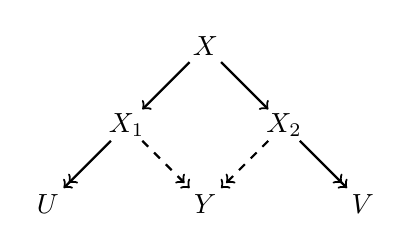
\begin{tikzpicture}
    \draw ( 0, 0) node {$X$};
    \draw (-1,-1) node {$X_1$};
    \draw ( 1,-1) node {$X_2$};
    \draw ( 0,-2) node {$Y$};
    \draw (-2,-2) node {$U$};
    \draw ( 2,-2) node {$V$};

    \draw[thick, ->] (-0.2,-0.2) -- (-0.8,-0.8);
    \draw[thick, ->>, dashed] (-0.8,-1.2) -- (-0.2,-1.8);
    \draw[thick, ->] (0.2,-0.2) -- (0.8,-0.8);
    \draw[thick, ->>, dashed] (0.8,-1.2) -- (0.2,-1.8);
    \draw[thick, ->>] (-1.2,-1.2) -- (-1.8,-1.8);
    \draw[thick, ->>] (1.2,-1.2) -- (1.8,-1.8);
  \end{tikzpicture}
\end{center}

Observe that $X_1$ has a smaller reduction tree than $X$. We can then use the induction hypothesis to see that $U$ and $Y$, and $V$ and $Y$ reduce to some terms $U_1$ and $V_1$:

\begin{center}
  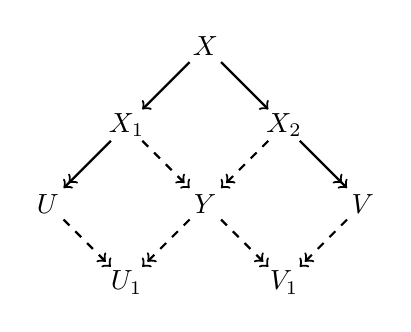
\begin{tikzpicture}
    \draw ( 0, 0) node {$X$};
    \draw (-1,-1) node {$X_1$};
    \draw ( 1,-1) node {$X_2$};
    \draw ( 0,-2) node {$Y$};
    \draw (-2,-2) node {$U$};
    \draw ( 2,-2) node {$V$};
    \draw (-1,-3) node {$U_1$};
    \draw ( 1,-3) node {$V_1$};

    \draw[thick, ->] (-0.2,-0.2) -- (-0.8,-0.8);
    \draw[thick, ->>, dashed] (-0.8,-1.2) -- (-0.2,-1.8);
    \draw[thick, ->] (0.2,-0.2) -- (0.8,-0.8);
    \draw[thick, ->>, dashed] (0.8,-1.2) -- (0.2,-1.8);
    \draw[thick, ->>] (-1.2,-1.2) -- (-1.8,-1.8);
    \draw[thick, ->>] (1.2,-1.2) -- (1.8,-1.8);

    \draw[thick,->>,dashed] (-1.8,-2.2) -- (-1.2,-2.8);
    \draw[thick,->>,dashed] ( 1.8,-2.2) -- ( 1.2,-2.8);
    \draw[thick,->>,dashed] ( 0.2,-2.2) -- ( 0.8,-2.8);
    \draw[thick,->>,dashed] (-0.2,-2.2) -- (-0.8,-2.8);
  \end{tikzpicture}
\end{center}

We now have $U_1$ and $V_1$, which by the inductive hypothesis eventually reduce to some term $W$ in a finite number of reductions. Additionally, that number of reductions is fewer than the number of reductions for $X$, so by the induction hypothesis we can claim that there exist reductions $U_1 \twoheadrightarrow_\beta W$ and $V_1 \twoheadrightarrow_\beta W$.

\begin{center}
  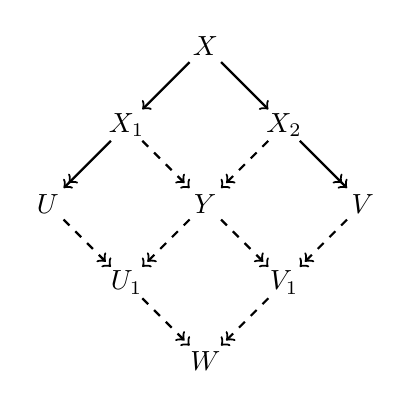
\begin{tikzpicture}
    \draw ( 0, 0) node {$X$};
    \draw (-1,-1) node {$X_1$};
    \draw ( 1,-1) node {$X_2$};
    \draw ( 0,-2) node {$Y$};
    \draw (-2,-2) node {$U$};
    \draw ( 2,-2) node {$V$};
    \draw (-1,-3) node {$U_1$};
    \draw ( 1,-3) node {$V_1$};
    \draw ( 0,-4) node {$W$};

    \draw[thick, ->] (-0.2,-0.2) -- (-0.8,-0.8);
    \draw[thick, ->>, dashed] (-0.8,-1.2) -- (-0.2,-1.8);
    \draw[thick, ->] (0.2,-0.2) -- (0.8,-0.8);
    \draw[thick, ->>, dashed] (0.8,-1.2) -- (0.2,-1.8);
    \draw[thick, ->>] (-1.2,-1.2) -- (-1.8,-1.8);
    \draw[thick, ->>] (1.2,-1.2) -- (1.8,-1.8);

    \draw[thick,->>,dashed] (-1.8,-2.2) -- (-1.2,-2.8);
    \draw[thick,->>,dashed] ( 1.8,-2.2) -- ( 1.2,-2.8);
    \draw[thick,->>,dashed] ( 0.2,-2.2) -- ( 0.8,-2.8);
    \draw[thick,->>,dashed] (-0.2,-2.2) -- (-0.8,-2.8);
    
    \draw[thick,->>,dashed] (-0.8,-3.2) -- (-0.2,-3.8);
    \draw[thick,->>,dashed] ( 0.8,-3.2) -- ( 0.2,-3.8);
  \end{tikzpicture}
\end{center}

This demonstrates that all reduction sequences of $X$ eventually terminate at some term $W$, which proves our claim. So all redution sequences of strongly normalizable terms are finite, and terminate in the same term.

\section{Simulating Strong Normalization}

\textbf{Digression:} $\infty$ reduction paths (or perpetual reduction paths). For some $X \not\in$ SN, find a principle redex in $X$, called $\Delta$ such that the contraction of $\Delta$ results in a term $Y \not\in$ SN.\\

Possible terms:
\begin{enumerate}
  \item The principle redex of $\l uU$ is the principle redex of $U$.
  \item $X = X_1,\ldots X_n$ has a principle redex of $X_i$ such that $i$ is the smallest such $i$ such that a redex exists.
  \item $X = (\l xX_0)X_1,\ldots,X_n$. If the head redex is contracted, then it is principle.
\end{enumerate}
The principle redex redex is

\begin{enumerate}[a.]
  \item if $x \not\in FV(X_0)$, then the principle redex of $X$ is the principle redex of $X_1$, if it exists.
  \item else $(\l xX_0)X_1$ is the principle redex.
\end{enumerate}

\textbf{Corollary:} If $X$ is not strongly normalizable, and $Y$ results by contracting the principle redex of $X$, then $Y \not\in$ SN.\\

\textbf{Definition:} Comparing redexes in $X$. Standardizations says that you should always contract a redex able on to the left of the anchor.

\subsection{On Coloring Redexes (A Simulation of SN)}
Given a term $X$, we color some (strict) subset of the redexes in $X$ green. An uncolored redex is red. If $X$ reduces to $Y$ in a single step by some green redex $\Delta$, then the redexes in $Y$ which are residuals of those in $X$ which are green get colored green. We call this a \textbf{Colored Reduction}\index{Colored Reduction|textbf}.\\

If $X \rightarrow_{\beta, colored} Y$, and $Y$ has no colored redexes, then $Y$ is said to be a complete development of green redexes in $X$.\\

\textbf{Theorem (Hindley):}\index{Hindley's Theorem} Every colored reduction sequence terminates in a unique normal form. Note that we have weak diamond for colored reductions.
\begin{center}
  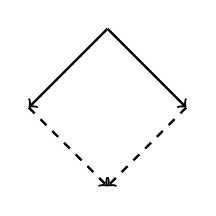
\begin{tikzpicture}
    \draw[thick, ->] (0,0) -- (-1,-1); % X
    \draw[thick, ->, dashed] (-1,-1) -- (0,-2); % U by Delta_1
    \draw[thick, ->] (0,0) -- (1,-1); % V by Delta_2
    \draw[thick, ->, dashed] (1,-1) -- (0,-2); % W by residuals of Delta_1 and Delta_2
  \end{tikzpicture}
\end{center}

\textbf{Proof:} $X \mapsto \# X$ and a colored reduction to $Y$ gives us $Y \mapsto \# Y$ for some $\#$ which associates a nonnegative integer with terms.
\chapter{Lecture 14}
\lhead{February 13, 2015}
\chead{21-366 Lambda Calculus Lecture 14}

\section{Valuation on a Term $X$}
\index{Valuation|textbf}
During the previous lecture we mentioned a function which mapped terms to nonnegative integers. Now we formalize that idea as the valuation of a term, and give some restrictions on what forms a valuation can take. A valuation on a term is a map $\v : \hbox{subterms}(X) \rightarrow \mathbb{N}^+$ satisfying two conditions:

\begin{itemize}
\item The value $\v(x) > \sum_{T\hbox{ to the right of }x}\v(T)$ in a redex in $R$. So for $(\l uU)V$, $\v(u) > \v(U)$.
\item $\v((UV)) > \hbox{max}(\v(U),\v(V))$ and $\v(\l uU) > \v(U)$
\end{itemize}

Valuations exist for any term. Assume by recursion that
\begin{itemize}
  \item All leaves to the right of $x$ have values
  \item All subterms all of value variable occurance have values themselves have values. (What?)
\end{itemize}

Given a valuation of $X$,
\begin{equation*}
  \# X = \sum_{Y\hbox{ a subterm of }X}\v(Y)
\end{equation*}

\subsection{Colored Reductions}
\index{Colored Reduction|textbf}
Select some subset $R$ of the set of redexes in a given term $X$ and color them green. Color all others red. We defined last time colored reductions $X \rightarrow X_o {{\Delta_1} \atop {\rightarrow_\beta}} X_1 {{\Delta_2} \atop {\rightarrow_\beta}} \ldots$ where $\Delta_1 \in R$, and $\Delta_2 \in$ residuals of $R$.\\

\textbf{Claim:} There exists a valuation on $X_1$ induced by the reduction $X_0 {{\Delta_1} \atop {\rightarrow_\beta}}$ such that $\# X_1 < \# X_0$.\\

\textbf{Proof:} Consider a redex $\Delta_1 \in R$...\\

\textbf{Conclusion:} Every colored reduction sequence terminates. This gives us that every colored reduction sequence terminates in a unique ``normal form'' with no colored redexes. We call these colored reductions ``complete development.''

\subsection{The Lemma of Parallel Moves}
\index{Strip Lemma|textbf}
This is also known as the Strip Lemma. If we have a reduction of the form
\begin{center}
  \begin{tikzpicture}
    \draw (-1,-1) -- (0,0) -- (1,-1); % Left is many reductions, Right is one.
    \draw[dashed] (-1,-1) -- (0,-2) -- (1,-1);
  \end{tikzpicture}
\end{center}

\textbf{Remark:} Church-Rosser follows by induction on the conversion. With many and one, we can repeatedly apply until we get many and many.\\

\subsection{Proof of the Strip Lemma}

\chapter{Lecture 15}
\lhead{February 16, 2015}
\chead{21-366 Lambda Calculus Lecture 15}

\section{Review}
The finiteness of developments results in a unique ``normal form.''\\

\textbf{Strip Lemma (the Lemma of Parallel Moves):}\index{Strip Lemma} A single reduction $\Delta$ and a $\beta$ reduction followed by a complete reduction of all the residuals of $\Delta$ can be reached by $\beta$ reducing the term after applying $\Delta$.
% Picture line 1: <<---- {\Delta \atop --->}
% Picture line 2: {complete reudction of all residuals of \Delta \atop ---->>} \dashed <<----

\section{Cofinal Reduction Strategies}
Assign to each term a reduction sequence
\begin{equation*}
  x = x_1 \rightarrow_\beta x_2 \rightarrow_\beta x_3 \rightarrow_\beta \ldots
\end{equation*}
So any $Y$ such that $X =_\beta Y$ is $\beta$ reduceable to some term in the sequence.\\

\subsection{Klop's Theorem}
\index{Klop's Theorem}
\textbf{Theorem (Jan Willem Klop):} A reduction sequence $x = x_0 \rightarrow_\beta x_1 \rightarrow_\beta \ldots$ is cofinal if for any $\Delta$ redex in any $x_i$, eventually there is a $j > i$ such that $\Delta$ has no residual in $x_j$.\margnot{Jan Willem Klop}{ Klop was born in 1945 in Gorinchem, Netherlands. He works on the Algebra of Communicating Processes at Vrije Universiteit, in Amsterdam.}\\

\textbf{Correlary:} The following sequence is cofinal:
\begin{equation*}
  x_1 \twoheadrightarrow_{\beta\hbox{ complete reduction of all redexes in $x_1$}} x_2 \twoheadrightarrow_{\beta\hbox{ complete reduction of all redexes in $x_2$}} \ldots
\end{equation*}

\textbf{Proof:} Suppose that the reduction sequence
\begin{equation*}
  x = x_0 \rightarrow_\beta x_1 \rightarrow_\beta \ldots
\end{equation*}
has the quality that for a redex $\Delta$ in $x_i$ there exists some $x_j$, $j > i$ such that $\Delta$ has no residual in $X_j$. Therefore, there exists some $k > i$ such that there are no redexes in $x_i$ have residuals in $x_k$. Now we prove that this reduction sequence is cofinite. Given $Y =_\beta x =_\beta x_0$, then by Church-Rosser, there exists a $Z$ such that $X \twoheadrightarrow_\beta Z \twoheadleftarrow_\beta Y$. We will show that there exists an $i$ such that $Z \twoheadrightarrow_\beta X_i$. We have that
\begin{equation*}
  Z \stackrel{\mathscr{R}}{\twoheadleftarrow_\beta} x_0 \rightarrow x_1 \rightarrow \ldots \rightarrow x_i \rightarrow \ldots
\end{equation*}

We induct on the length of the reduction sequence $\mathscr{R}$ from $X$ to $Z$. Basis: take the one redex $\Delta$ in $\mathscr{R}$. Let $i = 0$. Then there exists $j > 0$ such that $X_j$ has no residuals of $\Delta$ by the strip lemma.\\

We now consider for our induction step that $\mathscr{R}$ has a length greater than $1$.
\begin{equation*}
  \ldots \leftarrow_\beta x_i \leftarrow_\beta \ldots \leftarrow_\beta x_1 \leftarrow_\beta x_0 \twoheadrightarrow_\beta U \rightarrow_\beta(\Delta)\ Z
\end{equation*}
Take the last reduction, $\Delta$ in $\mathscr{R}$. By the induction hypothesis, there exists an $n$ such that $U \twoheadrightarrow X_n$. Let $C$ be the set of residuals of $\Delta$ in $X_n$. There exists a $k > n$ such that no ersidual of $C$ has $X_k$ a residual in $X_n$.\\

\section{A Method to Prove that $X \not=_\beta Y$}
We will generalize colored reductions. The idea, due to J.~J.~Levy, is called Levy labels.\index{Levy labels}\\

The general idea of Levy labels is that if we have a term $X$, we assign nonnegative integers to the subterms of $X$, representing the ``potential to reduce.'' Colored reduction simply assigned all ``red'' redexes $0$, and ``green'' redexes $1$, saying they had the potential for one reduction.\\

For our purposes, we will instead use finite sequences of integers. These sequences are nonempty, and the integers themselves are nonnegative. These sequences additionally obey the following property: $n_{i + i} = n_i \pm 1$.

\begin{equation*}
  n_1,n_2,n_3,\ldots n_k
\end{equation*}
\begin{itemize}
  \item $n_i \geq 0$
  \item $n_{i + i} = n_i \pm 1$
  \item $k > 0$
\end{itemize}
If $Y$ is a subterm of $X$, we will write $Y = Y^\alpha$, where $\alpha = n_1\ldots n_k$. We require that all occurances of a given variable $X$ should always have the same first element in the sequence $x = x^{n\alpha}$. The $\alpha$s may vary. Applications look like:
\begin{equation*}
  (U^{\alpha,{n+1}},V^{\beta,n})^{n,\gamma}
\end{equation*}
Abstractions look like:
\begin{equation*}
  (\l x^{n} X^{\alpha,n})^{n + 1,\gamma}
\end{equation*}
\chapter{Chapter 16}
\lhead{February 20, 2015}
\chead{21-366 Lambda Calculus Lecture 16}

\section{* The Book on Levy Labels}
TODO: find a copy of the textbook.

\section{Potential of a Term}
The potential function maps from subterms (occurances) to sequences of nonnegative integers $\alpha = n_1n_2\ldots n_k$ such that $n_{i+1} = n_i \pm 1$.\\

We write $Y = Y^\alpha$. The superscript is for the potential of $Y$. This satisfies
\begin{itemize}
  \item (Uniformity) For every variable occurance of $x$ the potential \uline{begins} with the same integer $x^{n\alpha}$.
  \item (Construction)
    \begin{itemize}
      \item Application: $(U^{\alpha,n+1}V^{\beta,n})^{n,\gamma}$
      \item Abstraction: $(\l u^{n,} U^{\beta,n})^{n+1,\gamma}$
    \end{itemize}
\end{itemize}

\textbf{Example:}
\begin{equation*}
  (\l x (x^3 x^{3,2})^{2,3})^4
\end{equation*}

\textbf{Proposition:} Every term has at least one pootential assignment where all potentials are $\geq$ any nonegative integer.\\

\textbf{Proof:} Let some integer $N$ be nonnegative. We assign to each variable $x$ the potential $N + 1$. If we have $U = U^{\alpha, N+1}$ and $V = V^{\beta, N+1}$. Then
\begin{eqnarray*}
  (U^{\alpha,N+1}V^{\beta,N+1,N})^{N,N+1}\\
  (\l u^{N+1}U^{\alpha,N+1})^{N+2,N+1}\\
\end{eqnarray*}
Beta reduction looks like:
\begin{equation*}
  ((\l x^{\alpha,} X^{\alpha,n})^{n+1 Y^{\beta, n}})^{n,\gamma}
\end{equation*}
Most generally, we could have
\begin{equation*}
  ((\l x^{n,} X^{\alpha,n})^{n+1,\delta,n+1} Y^{\beta,n})^{n,\gamma}
\end{equation*}
but we do not do this. We can simply do
\begin{equation*}
  ((\l x^{\alpha,} X^{\alpha,n})^{n+1 Y^{\beta, n}})^{n,\gamma} \rightarrow [Y^{\beta,n}/x^{n,}]X^{\alpha,n,\gamma}
\end{equation*}

\subsection{Potential Reduction}
\begin{equation*}
  (U^{\alpha,n+2,n+1}V^{\beta,n})^{n,\gamma} \rightarrow (U^{\alpha,n+2}V^{\beta,n,n+1})^{n+1,n,\gamma}
\end{equation*}
\begin{equation*}
  (U^{\alpha,n+1,n+2}V^{\beta,n+1})^{n+1,\gamma} \rightarrow (U^{\alpha,n+1}V^{\beta,n+1,n})^{n,n+1,\gamma}
\end{equation*}

\textbf{Example:}
let
\begin{equation*}
  \omega^4 = (\l x^3 (x^3x^{3,2})^{2,3})^4.
\end{equation*}
Then if we want to reduce $\Omega = \omega\omega$, we do
\begin{eqnarray*}
  \omega^4\omega^{4,3} &\rightarrow& (\omega^{4,3}\omega^{4,3,2})^{2,3,4} \rightarrow \omega^4 \omega^{4,3,2,3} \rightarrow \omega^{4,3,2,3}\omega^{4,3,2,3,2} \rightarrow \omega^{4,3,2} \omega^{4,3,2,3,2,1}\\
  &\rightarrow& \omega^4 \omega^{4,3,2,3,2,1,2,3} \rightarrow \omega^{4,3,2,3,2,1,2,3}\omega^{4,3,2,3,2,1,2,3,2}\\
  &\rightarrow& \omega^{4,3,2,3,2,1} \omega^{4,3,2,3,2,1,2,3,2,1,0}\\
\end{eqnarray*}

We now have two kinds of reductions: beta reductions and potential reductions.\\

\textbf{Definition:} We say that a term with potential is \uline{strongly normalizable} if every alternating sequence of beta reductions and potential reductions terminates.\\

\textbf{Theorem:} Every term is strongly normalizable.
\chapter{Lecture 17}
\lhead{February 23, 2015}
\chead{21-366 Lambda Calculus Lecture 17}

\section{Reduction of Terms with Potential}
Recal that a potential is a sequence of nonnegative integers $n_1,n_2,\ldots,n_k$ such that $n_{i+1} = n_i \pm 1$. We now have three kinds of reductions we can perform:

\begin{eqnarray*}
  &\hbox{\hspace{.27in}\uline{Beta:} }& (1)\ \ ((\l x^{n,} X^{\alpha,n})^{n+1}Y^{\beta,n})^{n,\gamma} \rightarrow_\beta [Y^{\beta,n}/x^{n,}]X^{\alpha,n,\gamma}\\
  &\hbox{\uline{Potential:} }& (2)\ \ (U^{\alpha,n+2,n+1} V^{\beta,n})^{n,\gamma} \rightarrow (U^{\alpha,n+2} V^{\beta,n,n+1})^{n+1,n,\gamma}\\
  && (3)\ \ (U^{\alpha, n+1, n+2} V^{\beta,n+1})^{n+1, \gamma} \rightarrow (U^{\alpha, n+1} V^{\beta,n+1,n})^{n,n+1,\gamma}
\end{eqnarray*}
The above potential reductions are oftentimes referred to as ``rotations.''\\

Recall that we introduced potentials as a generalization of the idea of colored reductions. This raises a question: what corresponds to the case of colored redexes? We define every variable $x$ to have a potential of zero: $x^0$. Every instance of lambda abstraction gives us then $(\l x^0X^0)^{1,0}$. Our reductions stall, as this gives us $U^{0,1}V^2$.\\

If we assign a variable a potential of $1$, then our reductions do not stall. So this corresponds to a colored reduction. We have $U^1,V^1$.

\subsection{Weak Diamond with Potential Reduction}
We now consider a case where we have two terms $U$ and $V$ which both can be reduced using \textit{either} beta reduction or potential reduction from some third term $X$. The weak diamond property also holds in this case.
\begin{center}
  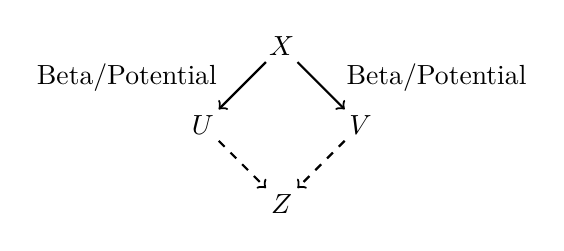
\begin{tikzpicture}
    \draw (0,0) node {$X$};
    \draw (-1,-1) node {$U$};
    \draw (1,-1) node {$V$};
    \draw (0,-2) node {$Z$};

    \draw[thick,->] (-.2,-.2) -- (-.8,-.8);
    \draw[thick,->] (.2,-.2) -- (.8,-.8);
    \draw[thick,dashed,->] (-.8,-1.2) -- (-.2,-1.8);
    \draw[thick,dashed,->] (.8,-1.2) -- (.2,-1.8);

    \draw (-.7,-.4) node[anchor=east] {Beta/Potential};
    \draw (.7,-.4) node[anchor=west] {Beta/Potential};
  \end{tikzpicture}
\end{center}

\textbf{Proof:} Consider $\Delta_1$ and $\Delta_2$ as $\beta$ redexes. There are four possible cases:
% The usual weak diamond picture with \Delta_1 and \Delta_2 as redexes
\begin{center}
  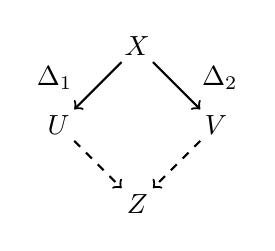
\begin{tikzpicture}
    \draw (0,0) node {$X$};
    \draw (-1,-1) node {$U$};
    \draw (1,-1) node {$V$};
    \draw (0,-2) node {$Z$};

    \draw[thick,->] (-.2,-.2) -- (-.8,-.8);
    \draw[thick,->] (.2,-.2) -- (.8,-.8);
    \draw[thick,dashed,->] (-.8,-1.2) -- (-.2,-1.8);
    \draw[thick,dashed,->] (.8,-1.2) -- (.2,-1.8);

    \draw (-.7,-.4) node[anchor=east] {$\Delta_1$};
    \draw (.7,-.4) node[anchor=west] {$\Delta_2$};
  \end{tikzpicture}
\end{center}
\begin{enumerate}[(1)]
  \item $\Delta_1$ and $\Delta_2$ are disjoint. This case is equivalent to the one without potentials.
  \item $\Delta_1$ is contained in $\Delta_2$
  \begin{enumerate}[(a)]
    \item $\Delta_1$ is contained in argument
    \item $\Delta_1$ is contained in abstraction terms
  \end{enumerate}
  \item Rotation/Rotation with $\Delta_1 \subseteq \Delta_2$. The diagram can be completed as in the case without potential.
  \item Rotation/Beta. There can be no conflict between a rotation and a beta reduction.
\end{enumerate}

\textbf{Definition:} We say that $X^{\alpha}$ is strongly normalizable SN if every reduction sequence terminates.

\section{Perpetual Strategy}
We define a \uline{principle redex} $\Delta$ such that if $X = X_0 \rightarrow X_1 \rightarrow X_2 \rightarrow \ldots \rightarrow X_n \rightarrow \infty$ sequence, then there is one with $\Delta$ as the first redex.\\

The principle redex of a term $X$ is
\begin{enumerate}[(1)]
  \item $X = (\l y^{n,}Y^{\beta,n})^{n+1,\alpha}$, then the principle redex is $Y^{\beta,n}$.
  \item $X = ((x^{\alpha,n+1}X_1^{\beta,n,})^{n_1}X_2^{\beta_2,N_1-1})\ldots X_n^{\boxed{\hphantom{lol}}}$, then
    \begin{enumerate}[(a)]
      \item The first $i$ such that $X_i$ has a principle redex.
      \item Else the principle redex is $x^{\alpha,n_+1}X_1^{\beta,n}$ if (1) or (2) apply
    \end{enumerate}
\end{enumerate}
\chapter{Lecture 18}
\lhead{February 25, 2015}
\chead{21-366 Lambda Calculus Lecture 18}
\rhead{Brian Jacobs}

\section{Lexicographic Orderings}
\margnot{Alphabetic Ordering}{ The lexicographic ordering is a generalization of the idea of alphabetic ordering. Alphabetic ordering is just a lexicographic ordering where the tuple is the letters of the strings and the ordering is based on where in the alphabet letters occur.}
A problem which sometimes arises is the problem of ordering tuples of the form $(x_0,\ldots,x_n)$ where the individual elements $x_i$ have some ordering such that we can say $x_i = x_j, x_i < x_j$ or $x_i > x_j$. There are a number of ways that we could go about this, so we start by making a list of properties that we wish lexicographic ordering to have. Ideally, our ordering will tell us that identical lists are equal and anything else is not, and be transitive.\\

An obvious first approach would be to simply say that for two tuples $X$ and $Y$ we will compare the first two elments $x_0$ and $y_0$. If $x_0 > y_0$, then $X > Y$, and so forth. We have to decide, however, what to do in a case where the length of $X$ and the length of $Y$ differ, as in the case where $X = (x_0,x_1,x_2)$ and $Y = (y_0,y_1)$. We can pad one of the tuples until it is equal in length to the other with elements which are either greater or smaller than the elements of the two lists. So if the elements of $X$ and $Y$ are integers, we might say that
\begin{equation*}
  (x_0,x_1,x_2) \stackrel{?}{=} (y_0,y_1) \Longleftrightarrow (x_0,x_1,x_2) \stackrel{?}{=} (y_0,y_1,\infty)
\end{equation*}

\section{Definition of Principle Redex}
We claim that if an infinite reduction sequence exists for some term, we can find it by repeatedly contracting the principle redex of the term. The principle redex is defined in the following way:
\examplebox{Definition of Principle Redex}{
  \begin{enumerate}[(1)]
  \item $(\l x^{n,}X^{\alpha,n})^{n+1,\beta}$ is the principle redex of $X^{\alpha,n}$
  \item $(U^{\alpha,n+1} V^{\beta,n})^{n,\gamma}$ is the principle redex of
    \begin{enumerate}[(a)]
    \item $U^{\alpha,n+1}$ if $U$ is a variable or an application and the principle redex exists, else the principle redex of $V^{\beta,n}$
    \item if $U^{\alpha,n+1} = (\l y^{m}Y^{\delta,m})^{m+1,\alpha',n+1}$ then
      \begin{enumerate}[(i)]
      \item $\alpha'$ contains $0$, then the principle redex of $Y^{\delta,m}$ if it exists, else
      \item $y \not\in \FV(Y)$ then the principle redex of $V$ if it exists, else $Y$.
      \end{enumerate}
    \end{enumerate}
  \end{enumerate}
}

At this point [(1)(a)(ii)] we have a term of the form:
\begin{equation*}
  ((\l u^{n,}U^{\alpha,n})^{n+1,\beta,m+1}V^{\gamma,m})^{m,\delta}
\end{equation*}

\begin{enumerate}[(1)]
  \item 0 in $\beta$
  \item no $0$ in $\beta$, $u \not\in \FV(U)$ principlal redex to be the one for $V$ if it exists.
  \item Potential
\end{enumerate}

\subsection{Proof of Infinte Reduction of Principle Redex}
We want to demonstrate that the perpetual reduction strategy always contracts the principle redex.\\

\textbf{Lemma:} if $X^{\alpha} \in $ SN and $Y^{\beta,n} \in $ SN where $y^n \in \FV(X)$. It then makes sense to apply $[Y^{\beta,n}/y^{n}]X^{\alpha}$.\\

\textbf{Proof:} We first look at the special case of $Y^{\beta,n} = (xY_1\ldots Y_m)^{\beta,n}$. $X^{\alpha}$ is strongly normalizable, so the reduction tree of $X^\alpha$ is finite and of size $t$. $X^{\alpha}$ also has a length, $\ell$. We can induct on pairs $(t,\ell)$.

\begin{center}
  \begin{tikzpicture}
    \draw[thick,->] (-.5,0) -- (2,0);
    \draw[thick,->] (0,-.5) -- (0,2);
    \draw (0,1) node[anchor=east] {$t$};
    \draw (1,0) node[anchor=north] {$\ell$};
  \end{tikzpicture}
\end{center}

We establish a lexicographic ordering on the points whereby $(t,\ell) > (t',\ell')$ if $t > t'$ or if $t = t'$ and $\ell > \ell'$.\\

If $X = y$, then $\alpha = n,\alpha'$. So when we perform the substitution, we get
\begin{equation*}
  [Y^{\alpha,n}/y^n]X^{\alpha} = (xY_1\ldots Y_m)^{\beta,n,\alpha'}
\end{equation*}
Note that $Y^{\beta,n} \in \SN \Leftrightarrow Y_1,\ldots,Y_m \in \SN$.\\

\textit{Induction Step:} We have the following cases:
\begin{itemize}
  \item $X = zX_1\ldots X_k$ and $z \not= y.$
  \item $[Y/y]X = z([Y/y]X_1)\ldots([Y/y]X_{1_2})$ use $\ell$.
  \item $X = (\l zX_0)X_1\ldots X_k$.
  \item $[Y/y]X = (\l z [Y/y]X_0)([Y/y]X_1)\ldots([Y/y]X_k)$.
\end{itemize}

We now again have several cases: if $0$ is in the potential, then $z \not\in \FV(X_0)$  principle redex cases for $X_1$.
\chapter{Lecture 19}
\lhead{February? ???, 2015}
\chead{21-366 Lambda Calculus Lecture 19}
\rhead{Brian Jacobs}

\section{TODO: Find notes on this lecture}
\chapter{Lecture 20}
\lhead{March 2, 2015}
\chead{21-366 Lambda Calculus Lecture 20}
\rhead{Brian Jacobs}

\section{Closure of Strong Normalizable Terms Under Substitution}
We would like to show that for any strongly normalizable terms $X,Y$, the substitution $[Y/y]X$ is also strongly normalizable.

\subsection{Proof}
We can prove the claim by induction on the tuple $(p,r,t,\ell)$, where
\begin{center}
  \begin{tabular}{c l}
    $p$ & is the last integer in the potential of $Y$\\
    $r$ & is the size of the reduction tree of $Y$\\
    $t$ & is the size of the reduction tree of $X$\\
    $\ell$ & is the size of $X$\\
  \end{tabular}
\end{center}
\margnot{Lexicographic Ordering}{ Remember our definition of a lexicographic ordering from before. It allows us to induct on the tuple $(p,r,t,\ell)$ by giving us a formal description of when the tuple is getting ``smaller.''}

There are three options for the term $X$. It can either start with a variable $z$ which is not being substituted, a lambda term, or a variable $y$ which is being substituted.
\begin{eqnarray*}
  X &=& zX_1\ldots X_n\\
  X &=& (\l zZ)X_1\ldots X_n\\
  X &=& yX_1\ldots X_n\\
\end{eqnarray*}

For our third case, we have $[Y/y](X) = Y([Y/y]X_1)\ldots([Y/y]X_n)$. These $n + 1$ are in SN. We find the principle redex of $\Delta$ if $\Delta$ is a subterm of the first occurance of $Y$. We contract $\Delta$ in $Y$ to give $Y'$, so $\omega([Y/y]X_1)\ldots([Y/y]X_n)$, which is in SN by induction hypothesis on $r$. Note that this operation might increase $\ell$ or $t$, but it definitely reduces $r$ and does not affect $p$.\\

We have one more case: $Y = \l zZ$. We then have
\begin{eqnarray*}
  x = (y^{p,\alpha,m}X_1^{\beta,m})^{m,\gamma}\ldots
  Y &=& (\l z^s Z^{\delta,s})^{s + 1,\mu,p}
\end{eqnarray*}
let $[Y/y]X_1^{\beta,m}$ be $Z_1^{\beta,m}$. Then
\begin{eqnarray*}
  (\l z^sZ^{\delta,s})^{s+1,\mu,p,\alpha,m+1}Z_1^{\beta,m}
\end{eqnarray*}
We know that $Z_1$ is in SN by the induction hypothesis. Suppose $s + 1 = p$. Then we are substituting something with a last potential $p - 1$. Which would be nice, if it were true.\\

In case the potential $s+1,\mu,p,\alpha,m+1$ has a $0$ in it, it is not a principle redex. Then we get strong normalization from the induction hypothesis. Similarly, if $z \not\in \FV(Z)$ we also get strong normalization.\\

\textbf{Definition:} Shift and Rotate are funtions from potentials without zeros to potentials. The point of these functions is that: $(U^{p,\alpha} V^\beta)^\gamma$ potential reduces to $(U^{\beta} V^\delta)^\mu$ where $\delta = \beta$ rotate$(p,\alpha)$ and $\mu =$ shift$(p,\alpha)\gamma$.

{
  \def\rotate{\hbox{rotate}}
  \def\shift{\hbox{shift}}
  \begin{eqnarray*}
    \rotate(p) &=& \hbox{empty sequence}\\
    \shift(p) &=& \hbox{empty sequence}\\
    \rotate(\alpha,q+2,q+1) &=& q+1,\rotate(\alpha,q+2)\\
    \rotate(\alpha,q+1,q+2) &=& q, \rotate(\alpha,q+1)\\
    \shift(\alpha,q+2,q+1) &=& \shift(\alpha,q+2)q+1\\
    \shift(\alpha,q+1,q+2) &=& \shift(\alpha,q+1)q\\
  \end{eqnarray*}

}
\textbf{Fact:} $(U^{p,\alpha}V^\beta)^{\gamma}$ potential reduces to
\begin{equation*}
  (U^p V^{\beta,\hbox{\footnotesize rotate}(p,\alpha)})^{\hbox{\footnotesize shift}(p,\alpha),\gamma}
\end{equation*}
assuming $0$ is not in $p,\alpha$.\\

Back to the main thread of our proof, we have
\begin{eqnarray*}
  ((\l z^sZ^{\delta,s})^{s+1,\mu,p,\alpha,m+1}Z_1^{\beta,m})^{m,\gamma}\\
  ((\l z^sZ^s)^{s+1,\mu,p}Z_1^{\beta,m,\hbox{\footnotesize rotate}(p,\alpha,m+1)})^{m,\gamma,\hbox{\footnotesize shift}(p,\alpha,m+1)}
\end{eqnarray*}
Consider a new variable $w$ of potential $p-1,$rotate$(s+1,\mu,p)$. Consider the term $[w^{p-1,\hbox{\footnotesize rotate}(s+1,\mu,p)}/z^s]Z^s$. We know that this is in SN by the first part of the lemma, our original special case, or by induction hypothesis on $p$. \qqed
\chapter{Lecture 21}
\lhead{March? ???, 2015}
\chead{21-366 Lambda Calculus Lecture 21}
\rhead{Brian Jacobs}

\section{TODO: Find notes on this lecture}
\chapter{Lecture 22}
\lhead{March? ???, 2015}
\chead{21-366 Lambda Calculus Lecture 22}
\rhead{Brian Jacobs}

\section{TODO: Find notes on this lecture}
\chapter{Lecture 23}
\lhead{March 16, 2015}
\chead{21-366 Lambda Calculus Lecture 23}
\rhead{Brian Jacobs}

\section{Plan}
We have spent a while on theory, so now we spend some time on applications of fixed point combinators. Additionally, we have been talking a lot about $\beta$ reduction, but not about $\eta$ reduction, which we will now add. Furthermore, we will talk about Bohm's theorem, which answers the following question: For which sets of terms $S$ do we have a conditional $C$ i.e. if $X,Y \in S$ then $X = Y \Rightarrow CXY = K$ else if $X \not= Y \Rightarrow CXY = K_*$. Recall that $K = \l ab.a$ and $K_* = \l ab.b$. Put another way, this is the question of which sets of terms have a decidable equality.\\

\uline{B\"ohm's Theorem:} If $S$ is a set of normal forms, then there is a conditional $C$ for equality being beta-eta converstion.

\section{Demonstrating that Two Terms are Not Equal}

\examplebox{Curry and Turing's Fixed Point Combinators}{
\begin{eqnarray*}
  Y_C &=& \l y . (\l x y(xx)) (\l x y(xx))\\
  Y_T &=& (\l x . (\l y y(xxy)))(\l x . (\l y y(xyy)))
\end{eqnarray*}
\hphantom{a}
}
Can we show that $Y_C \not= Y_T$? The strategy for this is to pick a cofinal reduction sequence for one of the two terms. We will arbitrarily pick $Y_C$. If we have such a cofinal reduction sequence, and $Y_T$ reduces to some point in the cofinal reduction sequence of $Y_C$.
\begin{center}
  \begin{tikzpicture}
    \draw (0,0) node {$Y_C$};
    \draw[thick, dashed, ->>] (0,-0.2) -- (0,-1.8);
    \draw (2,0) node {$Y_T$};
    \draw[thick, dashed, ->>] (1.8,-0.2) -- (0.2,-1.8);
  \end{tikzpicture}
\end{center}

We see that we have a cofinal reduction sequence for $Y_C$:
\begin{equation*}
  \l (\l x y(xx))\underbrace{(\l x y(xx))}_{\alpha} \rightarrow \l y y(\alpha \alpha) \rightarrow \l y y(y(\alpha\alpha)) \twoheadrightarrow \ldots \twoheadrightarrow \l y \underbrace{y(\ldots y}_{n}(\alpha\alpha)) \ldots ) \twoheadrightarrow \ldots
\end{equation*}
By Klop's theorem, this sequence is cofinal. Also, notice that there is only redex to contract, so this reduction sequence is unique. We also can write a cofinal reduction sequence for $Y_T$:
\begin{equation*}
  \underbrace{\l x (\l y y(xxy))}_{\beta} \l x (\l y(xxy)) \rightarrow \l y y(\beta\beta y) \twoheadrightarrow\l y (y (y (\beta\beta y))) \rightarrow \ldots \rightarrow \l y \underbrace{y(y(\ldots*y}_{k}(\beta\beta y))\ldots)
\end{equation*}
We could alternately write from the point $\l y . y(y(\beta\beta y))$:
\begin{equation*}
  \l y . y(y(\beta\beta y)) \twoheadrightarrow \l y \underbrace{y(y(\ldots y}_{k}(\l z z(\beta\beta z))y))\ldots)
\end{equation*}
Notice that both reduction sequences continue with internal reductions. We can see that the internal reduction sequences are of terms which look like $y(\beta\beta y)$ and $(\l z z(\beta\beta z))y$. Neither of those can look like $(y(\alpha\alpha))$, so the terms $Y_C$ and $Y_T$ cannot be equal.

\subsection{Generalization by Corrado B\"ohm}
We define
\begin{equation*}
  Y_B = \underbrace{(\l x . (\l zy y(xxzy)))}_{\alpha} (\l x \l zy . y(xxzy))
\end{equation*}
by adding an extra parameter to $Y_C$. Recall that 
\begin{equation*}
  \uline{n} := \l xy.\underbrace{x(\ldots(x}_{n}y)\ldots)
\end{equation*}
We then define
\begin{equation*}
  Y_n = Y_B^{\uline{n}} \rightarrow (\l zy . y(\alpha\alpha zy))\uline{n} \rightarrow \l y . y(\alpha \alpha \uline{n} y) \twoheadrightarrow \l y . y(y(\alpha\alpha\uline{n}y)) \twoheadrightarrow \ldots
\end{equation*}
We can now observe that if $Y_n \not=_\beta Y_m$ for some $n \not= m$, we have infinitely many fixed point combinators.\\

\uline{Remark:} $F$ is a fixed point combinator if $\Leftarrow\Rightarrow Fx = x(Fx)$.\\ 

Exercise: Show that $Fx =_\beta x(Fx)$ is equivalent to $F =_\beta (\l y \l x (yx))F$. Start by abstracting both sides with a \l. Note: $(\l y \l x (yx))$ is called the owl combinator, so named by Ray Smullyan.

\section{Eta reduction}
Remember that if $x \not\in$FV$(X)$, then $\l x (Xx) \rightarrow_\eta X$. This is eta reduction. We also can define eta expansion:
\begin{equation*}
  X \rightarrow \l x(Xx) \hbox{ for } x \not\in \hbox{FV}(X)
\end{equation*}
\begin{enumerate}[(1)]
  \item Every eta reduction sequence terminates because lengths decrease
  \item Eta reduction has the diamond property.
\end{enumerate}
\begin{center}
  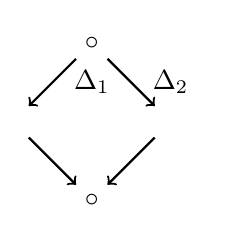
\begin{tikzpicture}
    \draw[thick, ->] (-0.2,-0.2) -- (-0.8,-0.8);
    \draw[thick, ->] (0.2,-0.2) -- (0.8,-0.8);
    \draw[thick, ->] (-0.8,-1.2) -- (-0.2,-1.8);
    \draw[thick, ->] (0.8,-1.2) -- (0.2,-1.8);

    \draw (0,0) node {$\circ$};
    \draw (0,-2) node {$\circ$};
    \draw (0,-0.5) node {$\Delta_1$};
    \draw (1,-0.5) node {$\Delta_2$}; % Add etas on the arrows
  \end{tikzpicture}
\end{center}
\textbf{Proof of (2):} Consider how $\Delta_1$ and $\Delta_2$ overlap. There can be no conflict.

\begin{enumerate}[(3)]
  \item Eta expansion has strong diamond
  \item Eta expansion has Church-Rosser
\end{enumerate}

\subsection{Eta expansion of terms with potential}
\begin{equation*}
  U^{\alpha,n+1,n+2,\beta} \stackrel{\hbox{\tiny eta expansion}}{\longrightarrow} (\l u^{n+1} (U^{\alpha,n+1}u^{n+1,n})^{n,n+1})^{n+2,\beta}
\end{equation*}
\chapter{Lecture 24}
\lhead{March 18, 2015}
\chead{21-366 Lambda Calculus Lecture 24}
\rhead{Brian Jacobs}

\section{Diamond Property for Reductions}
\subsection{Beta Reduction}
\subsection{Eta Expansion}
\begin{eqnarray*}
  U^{\alpha,n+1,n+2,\beta} &\rightarrow& (\l u^{n+1,n}(U^{\alpha,n+1}u^{n+1,n})^{n,n+1})^{n+2}\\
  U^{\alpha,n+2,n+1,\beta} &\rightarrow& (\l u^{n,n+1}(U^{\alpha,n+2}u^{n,n+1})^{n+1,n})^{n+1}
\end{eqnarray*}

\subsection{Potential Reductions}
\begin{eqnarray*}
  (U^{\alpha,n+1,n+2}V^{\beta,n+1})^{n+1,\gamma} &\rightarrow& (U^{\alpha,n+1}V^{\beta,n+1,n})^{n,n+1,\gamma}\\
  (U^{\alpha,n+2,n+1}V^{\beta,n})^{n,\gamma} &\rightarrow& (U^{\alpha,n+2}V^{\beta,n,n+1})^{n+1,n,\gamma}\\
  (\l u^{n,}U^{\alpha,n})^{n+1,n+2,\gamma} &\rightarrow& (\l u^{n+1,n}U^{\alpha,n,n+1})^{n+2,\gamma}\\
  (\l u^{n+1}U^{\alpha,n+1})^{n+2,n+1,\gamma} &\rightarrow& (\l u^{n,n+1}U^{\alpha,n+1,n})^{n+1}
\end{eqnarray*}
To prove the diamond property for reductions, any reduction tree without potential can be given potential.
\begin{enumerate}[(1)]
  \item Every $\beta$ reduction sequence terminates. (add clockwise rotation)
  \item Every eta expansion sequence terminates.
  \item Every potential reduction sequence terminates.
\end{enumerate}

\section{Tools for Proving Termination}
\subsection{Multiset Ordering}
A multiset is a set with multiplicity. Vaguely, a multiset is a finite set of natural numbers where each integer can occur more than once. The simplest example would be the set $\{n,n\}$, where the integer $n \in \mathbb{Z}$. A multiset is an assignment of nonnegative integers to the nonnegative integers, i.e. a function $f:\mathbb{N}\mapsto\mathbb{N}$ such that there exists $m \in \mathbb{N}$ such that for all $n \geq m, f(m) = 0$. A third definition: A multiset is a finite list of nonnegative integers modulo order.\\

We can order multisets as follows: $X > Y$ if there is an element $x \in X$ and a multiset $Z$ such that for each $z \in Z$, $z < x$ and $Y = X \setminus \{x\}$. That is to say, we say $X = \{\ldots,x,\ldots\}$ and $Z = \{z_1,\ldots,z_k\}$ for some $k \in \mathbb{N}$ and then do $X = \{\ldots,z_1,\ldots,z_k\ldots\}$.\\

\textbf{Theorem:} There is no infinite sequence of multisets $X_0 > X_1 > X_2 > \ldots > X_k > \ldots$. Recall K\"onig's Lemma: A tree which is finitely branching and infinite has an infinite path.\\

Suppose that we have an infinite descending sequence $X_n$ of multisets. A finitely branching tree of nonnegative integers. At any given stage the current $X_i = $ the leaves of this tree. Note that this tree has infinite nodes. However by K\"onig's lemma, this finitely branching tree must have an infinite path. This is a contradiction.\\
\chapter{Lecture 25}
\lhead{March 20, 2015}
\chead{21-366 Lambda Calculus Lecture 25}
\rhead{Brian Jacobs}

\section{Localization}
There are two types of local rotations, one for beta and one for eta.

\begin{enumerate}[(1)]
  \item (Eta) Given an eta expansion $U \rightarrow_\eta \l u(Uu)$ followed by any sequence of rotations, then the rotaions can be done first on the term containing just $U$. Except for local clockwise rotations. Those are of the following form, for example:
\end{enumerate}
\begin{eqnarray*}
  (\l u^{n,} (U^{\alpha,m+1,m+2}u^{n,\beta,m+1})^\square)^\diamond\\
  ((U^{\alpha,m+1}u^{n,\beta,m+1,m})^{m,\square})^\diamond
\end{eqnarray*}
Local means a clockwise rotation of the particular application $U \rightarrow_\eta \l u(Uu)$.\\

(2) (beta) Given beta reduction $(\l uU)V \rightarrow_\beta [V/u]U$. preceded by a seqnece of rotations. Then all the rotations can be done last, except local clockwise rotations of the redex.
\begin{eqnarray*}
  (\l u^{n,}U^{\alpha,n})^{n+1,n+2}V^{\delta,n+1}\\
  \rightarrow (\l u^{n+1,n}U^{\alpha,n,n+1})^{n+1}V^{\delta,n+1}\\ % Result of a counterclockwise rotation
  = [V^{\delta,m+1}/u^{n+1,n}]U^{\alpha,n,n+1}\\ % Further reduction
  ...\\
  \rightarrow (\l u^{n,}U^{\alpha,n})^{n+1}V^{\delta,n+1,n}\\ % Result of a clockwise rotation
  = [V^{\delta,n+1,n}/u^{n,}]U^{\alpha,n}
\end{eqnarray*}

\subsection{Eta Postponement}
If we have an eta expansion followed by a local clockwise rotation followed by a beta reduction, then these can be done in the ``opposite'' order: a local clockwise reduction followed by a beta reduction followed by a sequence of eta expansions.
\begin{equation*}
  (\l uU)V \rightarrow [V/u]U
\end{equation*}
Say that we have an eta expansion inside a term, $U \rightarrow \l uUu$, followed by some number of rotations local to the eta, followed by a beta reduction $(\l yY)z \rightarrow [Z/y]Y$.

% \Delta_1 : U -> \l u Uu -->> down(marked local to the eta) to \Delta_2 (\l yY)z -> [Z/y]Y

\textbf{Case 1:} $\Delta_1,\Delta_2$ are disjoint.\\
\textbf{Case 2:} Overlap:
2(a) $\Delta_1 \subseteq \Delta_2$ if $\Delta_1 = \Delta_2$ then we are clearly done in opposite order. If $\Delta_1 \subset \Delta_2$ and $\Delta_1 \subseteq Y$ $\Delta_1 \subseteq Z$ maybe many eta expansions in $[Z/y]Y$. $\Delta_1 = \l yY$ i.e. $UZ, \l u(Uu)Zm UZ$. Then simply keep $UZ$.\\

2(b) $\Delta_2 \subseteq \Delta_1$. There are several subcases: either $\Delta_2 = Uu$ or $\Delta_2 \subseteq U$ (This is another easy case). Now if $\Delta_2 = Uu$, then we get
\begin{eqnarray*}
  \l yY\\
  \l u((\l yY)u)\hbox{ clockwise rotations of $\l yY$ potentials onto $u$.}\\
  \l u([u/y]Y)\hbox{ net effect is a counterclockwise rotation}
\end{eqnarray*}

\textbf{Proof of Termination:} % TODO: IMPORT PROOF OF TERMINATION FROM WEBSITE
We need to show that:\\

(1) Every alternating sequence of beta reduction and clockwise rotations terminates.\\

(2) Every sequence of rotations terminates.\\

(3) Every sequence of eta expansions and clockwise rotations terminates.
\begin{eqnarray*}
  U^{\alpha,n+2,n+1,\beta}\rightarrow(\l u^{n,}(U^{\alpha,n+2}u^{n,n+1})^{n+1,n})^{n+1,\beta}
\end{eqnarray*}
We assign for each subterm the sum of the values of the potential. The value of the term equals the multiset of those sums.\\

Suppose we have an infinite sequence of betas, etas, and rotations. Take the first beta, and permute it to the beginning. You now have a number of local rotations, followed by a beta. We repeat this process until we have a sequence of local rotations, followed by a sequence of betas, followed by etas and rotations. This terminates, obviously. For the full, formal proof, see the appendix.
\chapter{Lecture 26}
\lhead{March 23, 2015}
\chead{21-366 Lambda Calculus Lecture 26}
\rhead{Brian Jacobs}
\pagestyle{fancy}

\section{Head Normal Form}
Recall: The general form of a term:
\begin{equation*}
  \l x_1\ldots x_n.x_1X_1\ldots X_m
\end{equation*}
with $n \geq 0, m \geq 0$ and $i \in \mathbb{N}$. This is called head normal form. The head variable is $x_i$.
\begin{equation*}
  \l x_1\ldots x_n(\underbrace{(\l x X_0)X_1}_{\hbox{head redex}}\ldots X_m)
\end{equation*}
with $n \geq 0$ and $m \geq 1$.\\

A term $X$ is said to have a head normal form $Y$ if $X =_\beta Y$ and $Y$ is in head normal form. This is highly nonunique.\\

Suppose that $Y$ is a head normal form, and $Y \twoheadrightarrow_\beta Z$. THen we know that $Z$ is also a normal form. It has the same lambda prefix $(n)$ and the same head variable $(i)$, and the same number of components $m$. Therefore if $X =_\beta Y$, $Y$ is in head normal form by church rosser.
\begin{equation*}
  X \twoheadrightarrow_\beta Z \twoheadleftarrow Y
\end{equation*}
Therefore, $X \twoheadrightarrow_\beta$ to a head normal form.\\

But $X \twoheadrightarrow_\beta Z$, where $Z$ is in head noraml form. In the head reduction part, $\l y_1,\ldots,y_r((\l yY_0)Y_1\ldots Y_s)$. $X \twoheadrightarrow_\beta W \twoheadrightarrow_\beta Z$.\\

\textbf{Theorem:} $X$ has a head normal form if and only if the head reduction sequence beginning with $X$ terminates.\\

\section{Solvability}
\textbf{Definition:} $X$ (a closed term) is said to be solvable if there exists terms $N_1\ldots N_n$ such that $XN_1\ldots N_n =_\beta I$.

\begin{eqnarray*}
  XN_1\ldots N_nK &=& K\\
  XN_1\ldots N_n &=& K\\
  XN_1\ldots N_n II &=& I\\
\end{eqnarray*}

\textbf{Theorem (Wadsworth):} A closed term $M$ is solvable if and only if $M$ has a head normal form.\\

% Note: make all the x_n.x_1 into x_n.x_i
\textbf{Proof:} $M$ has a head normal form $M \twoheadrightarrow_\beta \l x_1\ldots x_n . x_i X_1\ldots X_m$. Then
\begin{equation*}
  M\underbrace{K_*^m\ldots K_*^m}_{\hbox{$m$ times}} \twoheadrightarrow_\beta (\l x_1 \ldots x_n(x_1X_1\ldots X_m))K_*^m\ldots K_*^m \twoheadrightarrow_\beta K_*^m ([K_*^m/x_1,\ldots,K_*^m/x_n])\ldots \twoheadrightarrow_\beta I
\end{equation*}
Conversely, suppose that $M$ is solvable. $M N_1\ldots N_k  \twoheadrightarrow_{\hbox{head reduction }\beta} I$. We cannot reduce any subterms in such a way that $M$ is not in the head position.\\

\textbf{Remark:} $M$ is solvable if and only if there exists a term $F$ such that $FM = K_*$ and for some other term $N$, $FN =_\beta K$.\\

\textbf{Proof:} $M$ is solvable just like before. $F = \l u\ldots u K_*^m\ldots K_*^mFM \twoheadrightarrow_\beta K_*$. $FM = K_*$ and $FN = K$. We need two new variables $x,y$ so that $FMxy =_\beta Y$. $y$ is normal, so there is a head reduction $FMxy \twoheadrightarrow_\beta y$. $MW_1\ldots W_k \twoheadrightarrow_\beta y$.\\

Why does this prove that $M$ has a head normal form? Just put in $I$ for $x$ and $I$ for $y$ and you get $M([I/x,I/y]W_1)\ldots([I/x,I/y]W_k) \twoheadrightarrow_\beta I$.

\subsection{Properties of Unsolvable Terms}
Consider the following procedure on the possibly open term $X$. Perform the head reduction sequence. Either it does not terminate, in which case we have an open term with no head normal form. We call this $\bot$, or bottom. The option is that we get $\l x_1\ldots x_n.x_i$ We break $x_i$ into $X_1\ldots X_m$ and repeat in parallel, creating a finitely branching tree.
\begin{center}
  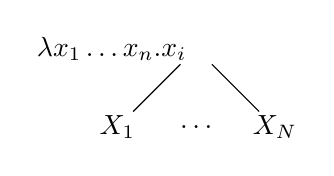
\begin{tikzpicture}
    \draw (0,0) node[anchor=east] {$\l x_1\ldots x_n.x_i$};
    \draw (-0.2,-0.2) -- (-0.8,-0.8);
    \draw (0.2,-0.2) -- (0.8,-0.8);
    \draw (-1,-1) node {$X_1$};
    \draw (0,-1) node {$\ldots$};
    \draw (1,-1) node {$X_N$};
  \end{tikzpicture}
\end{center}

This is called the Bohm tree of the term.

\section{Bohm Trees}
Facts and examples:
\begin{enumerate}[(1)]
  \item if $X$ has a noraml form, then the Bohm tree of $X$ is finite.
  \item any unsolvable term has a finite Bohm tree $= \bot$. For example, take $Y_TK$.
\end{enumerate}
Example: computing the Bohm tree of $Y_TK$.\\
\begin{equation*}
  Y_TK \twoheadrightarrow_\beta K(Y_TK) \rightarrow_\beta \l x(Y_TK) \twoheadrightarrow_\beta \l x_1\ldots x_n(Y_Tk)
\end{equation*}
We can see that this cannot have a head normal form, since we can have an arbitrarily large number of lambda prefixes. The Bohm Tree $BT(Y_TK) = \bot$.\\

\textbf{Remark:} $Y_TK$ is unsolvable, but it is not like $\Omega$. $\Omega$ cannot be reduced even to something beginning with a lambda. $\Omega \not\twoheadrightarrow_\beta \l xX$. $\Omega$ is still $\bot$.\\

A good Bohm tree, for example, looks like this: $M := \l x.Y_T(\l y.xy) \twoheadrightarrow_\beta \l x.x(Y_T/\l y.xy)$. Repeating this many times gives you $\twoheadrightarrow_\beta \l x.x(\ldots(x(Y_T(\l y.xy))))$. So the Bohm tree $BT(M)$ is:
\begin{tikzpicture}
  \draw (0,0) node[anchor=east] {$\l x.x$};
  \draw (0,0) -- (0,-1);
  \draw (0,-1) node {$x$}; % And so on...
\end{tikzpicture}
\chapter{Lecture 27}
\lhead{March 25, 2015}
\chead{21-366 Lambda Calculus Lecture 27}
\rhead{Brian Jacobs}
\pagestyle{fancy}

\section{B\"ohm Trees}
\textbf{Definition:} A B\"ohm tree is a finitely branching tree whose nodes are labeled
\begin{enumerate}[(1)]
  \item With a \l{} prefix and a head variable
    \begin{equation*}
      \l x_1\ldots x_n.x_i\ \ i\in \mathbb{N}
    \end{equation*}
  \item If the tree is a leaf, then
    \begin{equation*}
      \bot
    \end{equation*}
\end{enumerate}
We associate to each term $X$ a B\"ohm tree. If $X$ is unsolvable (that is, it has no head-normal form - by Wadsworth's Theorem), then the B\"ohm tree of $X$ is simply $\bot$. However if $X$ has a head normal form $\l x_1\ldots x_n . x_iX_1\ldots X_m$, then the B\"ohm tree of $X$ should be:
\begin{center}
  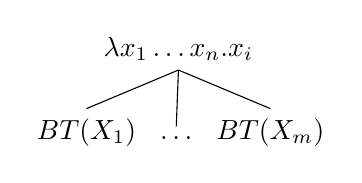
\begin{tikzpicture}
    \Tree[.$\l x_1\ldots x_n.x_i$ [.$BT(X_1)$ ] [.$\ldots$ ] [.$BT(X_m)$ ] ]
  \end{tikzpicture}
\end{center}

\textbf{Claim:} If $T = \hbox{BT}(X)$, then $T$ has finitely many free variables.\\

\textbf{Barendreight's theorem:} If a finitely bounded B\"ohm tree has finitely many free variables then it is the B\"ohm tree of a term. TODO: FIGURE OUT WHAT THIS IS CALLED AND FILL IT OUT.

\subsection{A Useful Ordering of B\"ohm Trees}
We say that $T_1 \sqsubseteq T_2$ if you can take $T_1$ and replace (possibly infintely many) $\bot$ nodes with arbitrary other B\"ohm trees.\\

Remark: $\sqsubseteq$ is a partial ordering. It is reflexive: $T_1 \sqsubseteq T_1$. It is transitive.\\

Remark: $T$ is finite.\\

Definition: $T_1$ and $T_2$ are \textbf{compatible} if there exists $T_1 \sqsubseteq T_3 \sqsupseteq T_2$.\\

Suppose that we have closed terms $M,N$ and a closed term $F$ such that $FM =_\beta K$ and $FN =_\beta K_*$. Then there exists a term with finite B\"ohm tree $M_1$ and a term $N_1$ with finite B\"ohm tree such that $BT(M_1) \sqsubseteq BT(M)$. We say that $M_1$ is an \textbf{approximation} of $M$. The same is true of $N$: $BT(N_1) \sqsubseteq BT(N)$.\\

Stated another way: IF there exists a term $F$ that can differentiate between $M$ and $N$, then it only needs to use a finite amount of the B\"ohm trees of $M$ and $N$ to do so. This idea is called \textbf{continuity}. This in particular is a weak form of continuity. Theoretically, we can put anything in place of $K$ and $K_*$, but if they have different B\"ohm trees, the theorem gets really hard to prove.\\


We have $FM =_\beta K$ and $FN =_\beta K_*$, so
\begin{eqnarray*}
  FMxy \stackrel{\hbox{head reduction}}{\twoheadrightarrow} x\\
  FNxy \stackrel{\hbox{head reduction}}{\twoheadrightarrow} y\\
\end{eqnarray*}

\textbf{Definition:} The levels of a B\"ohm tree. The root of a B\"ohm tree is level 1. Every subB\"ohm tree is of level 2.\\

\textbf{Proof:} Suppose that $FM =_\beta K$. THen $FMxy =_\beta x$. So $FMxy \twoheadrightarrow_\beta x$. Then there is an assignment of potentials $(FMxy)^{\alpha} \twoheadrightarrow_\beta x^{\alpha'}$. This is a normal form. By our theorem of Strong Normalization and uniqueness of normal form, we know that any reduction sequence of terms with potential beginning with $(FMxy)^\alpha$ must terminate in the term $x^{\alpha'}$. We can pick the reduction sequence which first puts $M$ in normal form as a term with potential. We call this new term $M'$.
\begin{equation*}
  M' = \l x_1\ldots x_n . \left\{
  \begin{tabular}{l}
    $x_i X_1\ldots X_m$\\
    or\\
    $(\l x X)^{0}X_1\ldots X_m$
  \end{tabular}
  \right.
\end{equation*}
If we have our first case case, the redex must be projected. In our second case we have a term with potential $0$ so, we simply replace it with $\bot$, as not it nor its residual can be constracted.\\

So $M_1$ is the result of replacing terms of the second kind with bottom. The B\"ohm tree of $M_1$ is therefore clearly less than or equal to the B\"ohm tree of $M$. $BT(M_1) \sqsubseteq BT(M)$.\\

It is then sufficient to consider terms with finite B\"ohm trees. \qqed\\

Next time we will codify properties of unsolvable terms.
\chapter{Lecture 28}
\lhead{March 27, 2015}
\chead{21-366 Lambda Calculus Lecture 28}
\rhead{Brian Jacobs}
\section{Continuity}
Recall: Suppose $M$ is closed and $XM =_\beta x$, a free variable. Then there exists a term $N$ with finite B\"ohm tree such that $BT(N) \sqsubseteq BT(M)$, and $XN =_\beta x$.\\

Claim: Suppose that $XN =_\beta x$ and the B\"ohm tree of $N$ is finite. Then whenever we have any term $M$ such that $BT(M) \sqsupseteq BT(N)$, then $XM =_\beta x$.\\

Proof: The B\"ohm tree of $N$ is obtained by repeatedly applying the standardization theorem until leaves of the tree are obtained. Once those leaves have been obtained, certain unsolvable terms are replaced by $\bot$. If we skip the final step, we have a reduct of $N$, say $N*$. We have $XN* \twoheadrightarrow_\beta x$. We can then replace those unsolvable leaves with $\Omega = (\l x.xx)(\l x.xx)$. The unsolvable terms are usually in the form $\l x_1\ldots x_n (\l xX)X_1\ldots X_m$. We now have a new term $N^+$ such that $XN^+ \twoheadrightarrow_\beta x$.\\

Clearly, then, if $BT(M) \sqsupseteq BT(N)$, then $XM \twoheadrightarrow_\beta x$.\\

Corollary: If $FM_1 =_\beta K$, and $FM_2 =_\beta K_*$, then $M_1$ and $M_2$ have incompatible B\"ohm trees. That is to say, there is no term $L$ such that $BT(M_1) \sqsubseteq BT(L) \sqsupseteq BT(M_2)$.\\

Proof: $FM_1 xy =_\beta x$ and $X = \l u(T uxy)XM_1 =_\beta x$. $FM_2xy =_\beta y$ $XM_2 =_\beta x$. Apply claim since we have $BT(L) \sqsupseteq BT(M_1) \sqsupseteq BT(M_2)$. $BT(M) \sqsupseteq BT(N)$\\

$XN_1* \twoheadrightarrow_\beta x$ \ \ \  $ BT(L) \sqsupseteq BT(N_1*)$\\
$XN_2* \twoheadrightarrow_\beta y$ \ \ \ $BT(L) \sqsupseteq BT(N_2*)$\\
Then there exists a finite term $L*$ such that $BT(L*) \sqsupseteq BT(N_1*)$ and $BT(L*) \sqsupseteq BT(N_2*)$. So we have that $XL* \twoheadrightarrow_\beta x$ and $XL* \twoheadrightarrow_\beta y$. This violates Church-Rosser.\\

Remark: Converse is false. For example, and 2 terms which eta convert cannot be ``split'' by such an $F$ ie if $M =_\beta N$ then you cannot have an $F$ such that $FM =_\beta K$ and $FN =_\beta K_*$. So, for example $\l xx =_\eta \l xy(xy)$. The B\"ohm tree of $\l x.x$ is $\l x.x$ and the B\"ohm tree of $\l (xy).(xy)$ is $\l xy. x --- y$.\\ % Make the line between x and y vertical, with y below x.

Eta is the only counterexample. Two finite B\"ohm trees are separable (splittable) only if one is not an eta conversion of the other.\\

\section{Properties of Unsolvables}
We say that a possibly open term $X$ is unsolvable if $X$ has no head normal form.\\

Remark: If $X$ is solvable then not necessarily the case that $M_1\ldots M_m XM_1\ldots M_m =_\beta I$. What is true is that there is a substitution $\Theta = [N_1/x_1,\ldots, N_n/x_n]$ where $FV(X) \subseteq \{X_1\ldots X_n\}$.\\

Recall that for all terms are either, $\l x_1 \ldots x_n. x_i X_1\ldots X_m$, $n \geq 0, m \geq 0, i \in \mathbb{N}$ (this is the head normal form) or $\l x_1\ldots x_n (\l xX)X_1\ldots X_m$ with $n \geq 0, m \geq 0$, which is not in head normal form.\\

\begin{enumerate}[(1)]
  \item Unsolvables are enumerable under reduction.
  \item If $X$ is unsolvable, then so is $\Theta X$ for any $\Theta$
\end{enumerate}
Proof: If the head reduction sequence of $X = X_1 \rightarrow_\beta X_2 \rightarrow_\beta \ldots \rightarrow_\beta X_k \rightarrow_\beta \ldots$ then the head reduction sequence of $\Theta X$ is $\Theta X_1 \rightarrow_\beta \Theta X_2 \rightarrow_\beta \ldots \rightarrow_\beta \Theta X_k \rightarrow_\beta \ldots$

\begin{enumerate}[(1)]
  \item 3 If and only if $X$ is unsolvable, then so is $\l x.X$.
  \item 4 If $X$ is unsolvable, and $Y$ is any term, then $XY$ is unsolvable.
\end{enumerate}
Proof: Let $X$ be unsolvable, and $Y$ a term. Consider a reductino sequence $XY \rightarrow_\beta X_0 \rightarrow_\beta X_1 \rightarrow_\beta X_2 \rightarrow_\beta \ldots \rightarrow_\beta X_k \rightarrow_\beta \ldots$. There are zero or more head reductions of $X$.\\

Case 1: $X$ does not head reduce to something beginning with a $\l$. Then this sequence is an infinite sequence.\\

Case 2: Consider ther first time a $\l$ comes to the head of $X$. We get $X = X_0$ and $X_0Y \rightarrow_\beta X_1Y \rightarrow_\beta \ldots \rightarrow_\beta X_kY \rightarrow_\beta (\l uU)Y \rightarrow_\beta [Y/u]U \rightarrow_\beta \ldots$. By property $3$, $\l uU$ is unsolvable, so $U$ is unsolvable. By condition $2$, $[Y/u]U$ is unsolvable, therefore $[Y/u]U$ from above is unsolvable and the following reduction is its head reduction sequence.\\

\subsection{Congruence}
\textbf{Definition:} \textbf{Congruence}: We define an -equivalence- congruence relation such that one subset of the equivalence relation is all unsolvables. We additionally want this equivalence relation to be closed under beta conversion. So $X \subseteq B, Y =_\beta X \Rightarrow Y \in B$. We partition into blocks closed modulo beta conversion: $X,Y \in B, U,V \in B \twoheadrightarrow XU, YV \in B$.\\
\chapter{Lecture 29}
\lhead{March 30, 2015}
\chead{21-366 Lambda Calculus Lecture 29}
\rhead{Brian Jacobs}

\section{Congruence}
\textbf{Definition:} A binary relation $\sim$ on closed terms is said to be a \textbf{congruence} if
\begin{enumerate}[(1)]
  \item $\sim$ is an equivalence relation
  \item closed under $\beta$ (and $\eta$). i.e. if $M =_\beta N \Rightarrow M \sim N$.
  \item $M \sim N$ and $P \sim Q \Rightarrow MP \sim NQ$
\end{enumerate}
Examples:
\begin{enumerate}[(i)]
  \item for all $M,N$ $M \sim N$
  \item $\{N : M \sim N\} = \{N : M =_\beta N\}$
  \item $\{N : M \sim N\} = \{N : M =_{\beta\eta} N\}$
\end{enumerate}
We know that example iii is not example i because of the Church-Rosser theorem: distinct normal forms don't $\beta\eta$ convert. iii and ii are different because $\beta$ conversion is not as exansive as $\beta\eta$ conversion.\\

Example: $\l xy.xy =_\eta \l x.x$ are in the same class for iii but have unique beta forms, so they are not in the same class for ii. The separation of i and ii is trivial. Take any two terms which do not $\beta$ convert.\\

Suppose that $S$ is a set of closed terms which are closed under $\beta$ conversion. Then there is a congruence relation $\sim$ such that if $M,N \in S$ then $M \sim N$. Indeed there is a smallest such $\sim$. i.e. for any other congruence $\backsim$, we have $M \sim N \Rightarrow M \backsim N$.Why? Because the intersection of congruences is a congruence.\\

\section{Jacopini's Theorem}
When are $M$ and $N$ related by the smallest congruence containing $S$ as a class?

\subsection{Jacopini Tableaus}
A \textbf{tableau} relating $M$ and $N$ consists of a sequence of terms $M_1,M_2,\ldots M_m$ and pairs of terms $(P_1,Q_1),(P_2,Q_2),\ldots,(P_m,Q_m)$ and the $\beta$ conversions
\begin{eqnarray*}
  M &=_\beta& M_1P_1Q_1\\
  M_1P_1Q_1 &=_\beta& M_2P_2Q_2\\
  M_2P_2Q_2 &=_\beta& M_3P_3Q_3\\
  &\vdots&\\
  M_{m-1}P_{m-1}Q_{m-1} &=_\beta& M_mP_mQ_m\\
  M_mP_mQ_m &=_\beta& N
\end{eqnarray*}
where $P_i, Q_i \in S$ such that $i = 1,\ldots,m$ and $m \geq 1$. An example is $S = \{Q : Q =_\beta P\}$.\\

Let $J$ be defined by $J(M,N)$ if and only if there is a Jacopini tableau linking $M$ and $N$. We now claim that $J$ is a congruence, and indeed is the smallest congruence.\\

Theorem:
\begin{enumerate}[(1)]
  \item J is a congruence
  \item If $\sim$ is a congruence containing $S$ as a class $J(M,N)$, then $M \sim N$
\end{enumerate}

Corellary: Let $\sim$ be the smallest congruence containing $S = $ the set of unsolvable terms as a class. Then if $M \sim N$ then $BT(M) = BT(N)$.\\

Example: $\Omega$ and $\Omega\Omega$ are both in $S$, but are $\beta$ different. So $\Omega \sim \Omega\Omega$. They have the same B\"ohm tree. In fact, $\l x .x\Omega \sim \l x. x(\Omega\Omega)$, and they have the same B\"ohm tree.\\

Proof: $M \sim N \Leftrightarrow$ there is a Jacopini tableau. Compute the B\"ohm tree $TB(M_i,P_i,Q_i)$. Compute a head normal form, if it exists.\\

Remark: Jacopini's Theorem: We can set $S$ to be the $\beta$ closure of $\{\Omega,M\}$, then the smallest $\sim$ containing $S$ as a class is not our first example from above.\\
\chapter{Lecture 30}
\lhead{April 1, 2015}
\chead{21-366 Lambda Calculus Lecture 30}
\rhead{Brian Jacobs}

\section{More on Jacopini}
For some $S$ a nonempty set of closed terms closed under $\beta$ equivalence, recall that $J(M,N) \Leftrightarrow$ there exist $M_1,\ldots,M_m$ which are closed, $P_1,\ldots P_m \in S$, $Q_1\ldots Q_m \in S$ such that
\begin{eqnarray*}
  M &=_\beta& M_1P_1Q_1\\
  M_1P_1Q_1 &=_\beta& M_2Q_2P_2\\
  \vdots\\
  M_mP_mQ_m &=_\beta& N
\end{eqnarray*}
NOTICE THAT THE Ps AND Qs SWITCH PLACES FROM ONE SIDE TO ANOTHER. 
Last time we introduced the Jacopini relation $J(M,N)$, which is a congruence which is closed under $=_\beta$. Today we show that it is the smallest.\\

Suppose that we are given $\sim$, a congruence such that if $P,Q \in S$, then $P \sim Q$. We want to show that if $J(M,N)$, then $M \sim N$.\\

Consider a case $M_iP_iQ_i = M_{i+1}P_{i+1}Q_{i+1}$. We have $J(M,M_1P_1Q_1)$ and $M \sim M_1P_1Q_1$. Why? $\sim$ is a congruence class, and the congruence classes are closed under $\beta$ conversion. Similarly, $J(M_iQ_iP_i,M_{i+1}Q_{i+1}P_{i+1})$ implies that $M_iQ_iP_i \sim M_{i+1}Q_{i+1}P_{i+1}$.\\

So we have some $M_iP_iQ_i$, now $M_iP_i \sim M_iP_i$, because congruence relations are reflexive. Secondly, we have $Q_i,P_{i+1} \in S$ by definition of tableau. Therefore $Q_i \sim P_{i+1}$. Therefore $M_iP_iQ_i \sim M_iP_iP_{i+1}$.

\subsection{Let us start over...}
We want to show that $M_iP_iQ_i \sim M_iQ_iP_i =_\beta M_iP_iQ_i \sim M_iP_iP_i$ since $Q_iP_i \in S$. We know that
\begin{equation*}
  \l x(M_i x Q_i)P_i\ldots
\end{equation*}

\subsection{Let us start over...}
We want to show that $M_iP_iQ_i \sim M_iQ_iP_i =_\beta M_iP_iQ_i \sim M_iP_iP_i$. We know that
\begin{equation*}
  M_iP_iQ_i \sim M_iP_iP_i =_\beta (\l x M_i x P_i) \sim (\l x M_i x P_i)P_iQ_i \in S
\end{equation*}
We are trying to prove that every step in the tableau equivalences remain in $S$.\\

We have a problem. If $S = \{K,K_*\}$. If we have $K \sim K_* \rightarrow_\beta M \sim N \Rightarrow KMN \sim K_*MN \rightarrow_\beta M \sim N$.

\section{B\"ohm's Theorem}
We will prove a bare bones version: If $M$ and $N$ are closed terms in normal form and they do not $\eta$ convert, then there exists terms $P_1\ldots P_n$ such that $MP_1\ldots P_m =_\beta K$ and $NP_1\ldots P_m =_\beta K_*$.\\

Remark: This is true for terms with finite B\"ohm trees.\\

\subsection{Proof}
The terms $M$ and $N$ look like:
\begin{equation*}
  \l x_1\ldots x_n.x_i
\end{equation*}
where $x_i$ has subterms $X_1\ldots X_m$. $n$ and $m$ can both be zero. There are three different ways in which a node in $M$ can differ from one in $N$. Different length lambda prefix, different length bound variables, ???.\\

Eta Expansion Example: $\l xy.xX \rightarrow_\eta \l xy.(\l z(xX)z)$ We could alternately reduce $\l xy.xX \rightarrow_\eta \l x \l z (\l y.xX)z$.\\

Notice that when we eta convert, the length of the lambda prefix and the number of bound variables both change. But they both change in such a way that $N - M$ is invariant.\\

We assume that $M,N$ are $M \not=_\eta N$ normal form with the same tree. Find the first place at which the B\"ohm trees are different. For example, suppose that at the root of the tree we have $M = \l x_1\ldots x_n . x_iX_1\ldots X_n$ and $N = \l y_1\ldots y_k . y_jY_1\ldots Y_k$. There are two cases.\\

Case 1: $n \not= k$, $n > k$ For each $P_1\ldots P_n$, $MP_1\ldots P_n = P_iX_1^+\ldots X_n^+$ and $NP_1\ldots P_n = P_jY_1^+\ldots Y_m^+P_{k+1}\ldots P_n$. How do we ensure that $P_i = P_j$? We set for all $r = 1,\ldots,n$ $P_r = \l z_1\ldots z_{n}I$. So $MP_1\ldots P_n =_\beta I$
\chapter{Lecture 31}
\lhead{April 3, 2015}
\chead{21-366 Lambda Calculus Lecture 31}
\rhead{Brian Jacobs}
\pagestyle{fancy}

\section{Proof of B\"ohm's Theorem}
\textbf{Recall:} $M$,$N$ in $\beta$-normal form. $M \not=_\beta N$.\\

\textbf{Claim:} There exists $P_1\ldots P_\ell$ such that
\begin{eqnarray*}
  MP_1\ldots P_\ell K\\
  NP_1\ldots P_\ell K_*\\
\end{eqnarray*}
\textbf{Remark:} By $\eta$ expansions we can assume that the B\"ohm trees of $M$ and $N$ are the same ``abstract'' tree. That is, the trees are the same without labels.\\

\textbf{Proof:} The proof is by induction on the depth of the first place where these two B\"ohm trees actually differ.\\

The basis case is when the two B\"ohm trees differ at the root, i.e. $M = \l x_1\ldots x_m.x_iX_1\ldots X_t$ and $\l y_1 \ldots Y_n . y_j Y_1\ldots Y_t$.\\

There are two cases.
\begin{enumerate}[(1)]
  \item $n \not= m$ so we assume without loss of generality that $m > n$
\end{enumerate}
We define
\begin{equation*}
  K_*^k := \l z_1\ldots z_k I
\end{equation*}
so that $K_*^1 = K_*$.
We then write for $r \geq t$
\begin{equation*}
  M\underbrace{K_*^{r}\ldots K_*^{r}}_{m} =_\beta K_*^{r}X_1^+\ldots X_t^+ =_\beta K_*^{r-t}
\end{equation*}
And
\begin{equation*}
  N\underbrace{K_*^{r}\ldots K_*^{r}}_{m} =_\beta K_*^{r}Y_1^+ \ldots Y_t^+ K_*^{r} \ldots K_*^{r} \rightarrow_\beta K_*^{r-t}\underbrace{K^r\ldots K^r}_{m - n} =_\beta K_*^{r-t+m-n}
\end{equation*}
Pick $r$ such that these two terms reduce to terms of the form $K_*^\alpha$ and $K_*^\beta$ where $\alpha \not= \beta$.\\

Assume $\alpha > \beta$. It suffices to find $Q_1\ldots Q_s$ such that $K_*^{\alpha}Q_1\ldots Q_s = K$ and $K_*^{\beta}Q_1\ldots Q_s = K_*$. Explicitly, these are $\l x_1\ldots x_\alpha . I Q_1\ldots Q_s$.\\

\textbf{Induction step:} Let
\begin{eqnarray*}
  M = \l x_1\ldots x_n . x_i X_1\ldots X_t\\
  N = \l x_1\ldots x_m . x_i Y_1\ldots Y_t\\
\end{eqnarray*}
Let $r$ be the smallest $1 \leq r \leq t$ such that the first place at which they differ is in the pair $X_rY_r$. Consider $x_iX_1\ldots X_t$ and $x_iY_1\ldots Y_t$. Pick an integer $\ell$ which is very large, i.e. $\ell >> t + t$. Substitute $\l y_1\ldots y_\ell \l a. a y_1\ldots y_\ell$ for $x_1$.
\chapter{Lecture 32}
\lhead{April 6, 2015}
\chead{21-366 Lambda Calculus Lecture 32}
\rhead{Brian Jacobs}

\section{G\"odel Numbering (without numbers)}
The idea is to assign to each lambda term $M$ at least one object, a G\"odel ``number'' (or code) which is another term $\godnum{M}$ (which is not necessarily unique) such that there exists a lambda term $E$, the evaluator, where
\begin{equation*}
  E\godnum{M} =_\beta M
\end{equation*}

Note that this gives us a fixed point theorem (oftentimes called the Kleene fixed point theorem). For each $M$ there exists an $N$ such that $N = M \godnum{N}$.\\

Corollary: There exists $N$ such that $MN =_\beta N$.\\

Since we can apply Kleene's fixed point to the term $\l x.M(Ex)$, we get an $N$ such that
\begin{equation*}
  MN =_\beta M(E\godnum{N}) =_\beta (\l x.M(Ex))\godnum{N} = N
\end{equation*}

\subsection{Proof of Kleene's Fixed Point}
Given $M$, consider the term
\begin{equation*}
  P = \l x.M(Exx)
\end{equation*}
Then
\begin{eqnarray*}
  P\godnum{P} =_\beta (\l x.M(Exx))\godnum{P} =_\beta M(E\godnum{P}\godnum{P}) = M(P\godnum{P})
\end{eqnarray*}

\subsection{Codes}
A code is a quadruple $\langle M,N,P,Q \rangle = \l a.aMNPQ$. There are three possible cases. Variable, application, or abstraction. $M$ tells us which we are in. It is one of the following:
\begin{eqnarray*}
  M = \begin{tabular}{c l}
    $\l abc.a$ & variable\\
    $\l abc.b$ & application\\
    $\l abc.c$ & abstraction\\
  \end{tabular}
\end{eqnarray*}
$N$ is a comment. We do not care what it is at present. $P$ is a placeholder which may be used later.\\

$Q$ is a church numeral $\uline{n}$ which tells us which variable it is. So, for example,
\begin{eqnarray*}
  \langle \l abc.a,N,P,\uline{n} \rangle &=& \godnum{X_n}\\
  \langle \l abc.b,N,\godnum{X},\godnum{Y} \rangle &=& \godnum{(X,Y)}\\
  \langle \l abc.c,N,\uline{n},\godnum{X} \rangle = \godnum{\l x_n.X}\\
\end{eqnarray*}
This defines the set of codes of terms.\\

\textbf{Remark 1:} Many functions on codes of terms will be defined by recursion. For example, we define the depth function.\\

Recall: there is a term MAX such that MAX$\ \uline{n}\ \uline{m} = \uline{\hbox{max}(n,m)}$. We define depth$\godnum{M} =$ a code of $M$ such that the comments are the depth of the corresponding subterm. So
\begin{equation*}
  \hbox{depth}(M) = \begin{tabular}{c l}
    $1$ & if $M$ is a variable\\
    $1 + \hbox{max}(\hbox{depth} X, \hbox{depth} Y)$ & if $M = XY$\\
    $1 + \hbox{depth}(X)$ & $M = \l x.X$
  \end{tabular}
\end{equation*}

\subsection{A Pidgeon Lambda Calculus Language}
We write $\godnum{M} = \langle P_0, P_1, P_2, P_3 \rangle$. If $P_0 = \l abc.a$, then $D\godnum{M} = \langle P_0, 1, P_2, P_3 \rangle$. If $P_0 = \l abc.b$, then $\langle P_0, \uline{+}\ \uline{1}\ \hbox{MAX} (D\godnum{P_2}(\l xyzw.y)) (D\godnum{P_3}(\l xyzw.y)), DP_2, DP_3 \rangle$. IF $P_0 = \l abc.c$, then $D\godnum{M} = \langle P_0, (DP_2(\l abced.b) + 1), P_2,P_3 \rangle$.\\

To make this a lambda term, we need to do two things. Replace the conditionals by projections, and then solve for $D$ using a fixed point combinator.
\chapter{Lecture 33}
\lhead{April 8, 2015}
\chead{21-366 Lambda Calculus Lecture 33}
\rhead{Brian Jacobs}

\section{Codes: A Review}
\begin{eqnarray*}
  \godnum{x_n} &=& \l a.ak_1^3MN\uline{n}\\
  \godnum{(XY)} &=& \l a.aK_2^3M\godnum{X}\godnum{Y}\\
  \godnum{\l x.X} &=& \l a.aK_3^3M\uline{n}\godnum{X}\\
\end{eqnarray*}
where
\begin{eqnarray*}
  K_i^n = \l x_1\ldots x_n.x_i\\
  \uline{n} = \l xy.\underbrace{x(\ldots (x}_{n}y)\ldots)
\end{eqnarray*}

\subsection{Examples}
\begin{eqnarray*}
  \godnum{K_i^n} &=& \langle K_3^3, \uline{0}, \uline{1}, \langle K_3^3, \uline{0}, \uline{2}, \langle \ldots \langle K_1^3, \uline{0}, \uline{0}, \uline{i} \rangle \rangle \ldots \rangle \rangle\\
  \godnum{\uline{n}} &=& \langle K_3^3, \uline{0}, \uline{1}, \langle K_3^3, \uline{0}, \uline{2}, \langle K_2^3, \uline{0}, \langle K_1^3, \uline{0}, \uline{0}, \uline{1} \rangle, \langle \godnum{\underbrace{x_1(\ldots(x_1}_{n-1}x_2))} \rangle \rangle \rangle \rangle
\end{eqnarray*}

\subsection{More Examples}
Recall our implementation of the stack. The empty stack, $\bot = \l a.K_*$. Push and pop and top. A stack of $X$'s look like $\l a.aX\square$ where $\square$ is a stack of $X$'s. The concatenation of two stacks, Cons $XY = $ if $x$ is $\bot$ then $y$; else push(top $x$) (cons pop$(x)$y).\\

pop$(\l a.aXY) = Y$ and top$(\l a.aXY) = X$.\\

\begin{equation*}
  Cons := Y_{Turing}\l xy.Test x((push(top x)(f (pop x)y))y)
\end{equation*}

\section{Simple Syntactic Functions}
FV$(\godnum{x})$? We write 
\begin{equation*}
  \godnum{x} = \langle K_i^3, M, P, Q \rangle
\end{equation*}
If $i = 1$, then we are in a variable case, and the free variables list is $\l a.aQ\bot$. If $i = 2$, then we have an application, and so the free variables list is the concatenation the free variables of $P$ and $Q$, or Cons FV$(P)$ FV$Q$. If $i = 3$, then we need to search the free variables of $Q$ and omit it. Otherwise, the free variables are the free variables of $Q$.\\

The bound variables are defined similarly.\\

$CV(X,x)$, assuming $x$ is a Church numeral. Search $X$ for $\l y$ such that $x$ is free, and list those $\l y$s.

\section{Substitution}
If we have $\godnum{X}$, $\godnum{Y}$, and $\godnum{x_n}$, then 
\chapter{Lecture 34}
\lhead{April 10, 2015}
\chead{21-366 Lambda Calculus Lecture 34}
\rhead{Brian Jacobs}
\pagestyle{fancy}

\section{Syntactic Functions}
\subsection{Depth First Search of a Code}
\begin{eqnarray*}
  D\godnum{X}x &=& \langle P,x,R,S \rangle \hbox{if $X = \langle P,Q,R,S \rangle$ is $P = K_1^3$}\\
  &=& \langle P, x, R, D S (Suc\ x) \rangle \hbox{if $P = K_3^3$}\\
  &=& \langle P, x, (DR(succ\ x)), \rangle
\end{eqnarray*}

\subsection{Alpha Conversion}
\begin{equation*}
  AL\godnum{X}\godnum{Y} = \begin{tabular}{c}$K$\\$K_*$\end{tabular}
\end{equation*}
depending on whether $Y$ is an $\alpha$ conversion of $X$.

\begin{equation*}
  EQ\godnum{X}\godnum{Y} = \begin{tabular}{c}$K$\\$K_*$\end{tabular}
\end{equation*}
Depending on whether $X = Y$.\\

Remark: There is no term $F$ such that $FMN = K$ iff $M =_\beta N$.\\

Suppose that $F$ exists. Consider the following term: let $G = Y_T(\l x.\lnot (FKx))$ for G\"odel. This imples that $G = (\l x.\lnot (FKx))G =_\beta \lnot(FKG)$. But $G = \lnot(F(KG)) = K_*$...

\chapter{Lecture 35}
\lhead{April 13, 2015}
\chead{21-366 Lambda Calculus Lecture 35}
\rhead{Brian Jacobs}
\pagestyle{fancy}

\section{Replacement and Substitutions}
\subsection{Kleene's Evaluator}
\begin{equation*}
  E_{Kleene}\godnum{M} =_{\beta} M
\end{equation*}
for some closed term $M$. $E$ is defined by recursion with a parameter $X$ which is a stack of the form $\langle \uline{n}, Z\rangle$ which tells us to substitute the term $Z$ for the free variable $x_n$. In pidgeon lambda calculus:\\

$F\godnum{Y}X =$ if $P = K_1^3$, then find $S$ in $X = Z$ and return it if it exists else return some random term, say $\Omega$. If $P = K_2^3$, then recurse with $(FRX)(FSX)$. If $P_3^3$, then $F\godnum{Y}X$ = $\l u.FS$Push$\langle R,u\rangle$.\\

Consider that things lower in the recursion will be accessed in the stack first. So the same variable can be bound int two different spots without problems.\\

We then define $F$ as a fixed point and set $E = \l a.Fa\bot$. For true codes, we can see that $E\godnum{M} =_\beta M$.\\

\subsection{Replacement}
We assume that $\godnum{X}$ has comments corresponding to depth first search. We want to define a term such that $REP\godnum{X}\godnum{Y}\uline{n}$ corresponds to the replacing of the subterm $X$ with dfs number $n$ by $Y$.\\

So if $P = K_1^3$, then if $Q = n$, return $\godnum{Y}$, and if $Q \not= n$, return $\godnum{X}$.

\subsection{Substitution}
$SUB\godnum{X}\godnum{Y}\uline{n} = 0$ substiutute $Y$ in $X$ for all free cocurances of $x_n$ in $X$. A question arises when bound variables are considered. $Y$ should be free for $x_n$ in $X$. $CV\godnum{X}\uline{n}$ is\footnote{$CV$ stands for conflicting variables.} a stack of variables bound on the paths to free occurances of $x_n$. If $X$ is a variable $x_k$, if $k = n$, then $\godnum{Y}$ else $\godnum{x_k}$.

\chapter{Lecture 36}
\def\floor#1{\lceil #1 \rceil}

\lhead{April 15, 2015}
\chead{21-366 Lambda Calculus Lecture 36}
\rhead{Brian Jacobs}
\pagestyle{fancy}

\section{Funtions Represented by \l{} Terms}
$\Phi : \mathbb{N} \mapsto \mathbb{N}$ partial functions where the domain of $\Phi \subsetneq \mathbb{N}$. Terms in particular $\{K,K_*\}$\\

Examples:
\begin{enumerate}[(1)]
  \item E(n,m) = \begin{tabular}{c}$K$ if $n = m$\\$K_*$ if $n \not= m$\end{tabular}
  \item O(n,m) = \begin{tabular}{c}$K$ if $n < m$\\$K_*$ if $n \geq m$\end{tabular}
  \item Closed under $\wedge,\vee,\neg$
  \item if $F$ represents a $\subset \mathbb{N}$ i.e. $F\uline{n} = K,K_*$, then $\exists_{<m} F = K$ if $\exists n F\uline{n} = K$ and $n < m$, and $\exists F = K_*$ if $\neg \exists n F\uline{n} = K$. Indeed if $\exists n F\uline{n} = K$, we would like to find the smallest such $n$. Kleene writes $\mu n F\uline{n} = k$, where $\mu$ represents min.
\end{enumerate}
Kleene called this general recursion. If we have $F,m$ such that $x \geq m$, $fx = K_*$. On the other hand, if $x < m$ and $Fx$, then $fx = K$. Finally, if $x < m$ and $\neg Fx$, then $fx = f \hbox{suc}x$. $\exists F = f\uline{0}$. We can unbound the search by ignoring the $x \geq m$ restriction.\\

\subsection{Examples}
Key application: there exists a term $L$ such that $L$ enumerates the codes of all terms. For each term $X$ there exists ($\infty$ many) $N$ such that $L n = \godnum{X}$.

\subsection{The Fundamental Theorem of Arithmetic}
Any natural number $n > 1$ can be written as the sum of powers of primes. A consequence of this theorem is that every natural number $n \geq 1$ can be written as a power of two times an odd integer. $n = 2^\alpha(4\beta \pm 1)$. Given some $n$, we can compute $\alpha,\beta$.\\

\begin{enumerate}[(1)]
  \item compute the relation $m | n$
\end{enumerate}
How? Euclid. $f mn = K$ if $n = m$, and $f (n - m)$ if $n > m$.\\

To compute the quotient and remainder of $n/m$
\begin{eqnarray*}
  n = Qm\bot R\\
  Q = \floor{\dfrac{n}{m}}\\
  R = n \monus \floor{\dfrac{n}{m}}
\end{eqnarray*}

\section{Construction of the Term $L$}
We will construcxt $\overline{L} n = $stack of the 1st $n$ terms.

\chapter{Lecture 38}
\lhead{April 22, 2015}
\chead{21-366 Lambda Calculus Lecture 38}
\rhead{Brian Jacobs}
\pagestyle{fancy}

\section{Notation}
Given a closed term $M$, $M$ ``defines'' a partial function $\phi_M : \mathbb{N} \mapsto \mathbb{N}$ where the domain of $\phi_M \subseteq \mathbb{N}$.

\begin{equation*}
  \phi_M(m) = n \Leftrightarrow M\uline{m} =_\beta \uline{n}
\end{equation*}

\subsection{Examples:}
\begin{enumerate}[(1)]
  \item $M = I$, so $\phi(m) = m$.
  \item $\Omega$ $\Omega\uline{m}$ has no normal form, so $\phi_m$ is undefined.
\end{enumerate}
Recall: We defined $S \subseteq \mathbb{N}$ is \textbf{recursively enumerable} if there exists $M$ such that
\begin{enumerate}
  \item $\phi$ is total
  \item The ring $\phi_M = S$
\end{enumerate}

More generally, suppose that $R \subseteq \mathbb{N}^n$.
\begin{eqnarray*}
  M_1,\ldots,M_n \in \mathbb{N}\\
  R(M_1,\ldots,M_n)
\end{eqnarray*}
Illustrate: $n = 2$. Definition. $R \in$ Recursively enumerable if...

\subsection{Pairing Function}
Bijection $\mathbb{N}^2 \Leftrightarrow \mathbb{N}$. Recall that every positive integer $k$ can be written as $2^\alpha(2\beta + 1)$. So $(\alpha,\beta) \leftrightarrow k+1 / k$.

\subsection{Properties of R.E. sets and relations}
\begin{enumerate}[(1)]
  \item R.E. sets are closed under $\cap,\cup$\\
    \textbf{Proof:} The union of recursively enumerable sets $S_1,S_2$, as terms $M_1,M_2$. $M =$ if $x = zy$ then $M_1y$, if $x = zy + 1$, then $M_2y$\\
    $sg(x \monus \lfloor\dfrac{x}{2}\rfloor \cdot 2)(M_1\lfloor\dfrac{x}{2}\rfloor)(M_2\lfloor\dfrac{x}{2}\rfloor)$\\
  \textbf{Intersection:} We assume that $S_1 \cap S_2 \not= \emptyset$. Find an integer $n \in S_1 \cap S_2$.\\
    \begin{eqnarray*}
      S_1 &=& \{n : \hbox{there exists }k_1\phi_{M_1}(k_1) = \}\\
      S_2 &=& \{n : \hbox{there exists }k_2\phi_{M_2}(k_2) = \}\\
      S_1 \cap S_2 &=& \{\phi_{M_1}(k_1) : \hbox{there exists }k_2\phi_{M_1}(k_1) = \phi_{m_2}(k_2)\}
    \end{eqnarray*}
    Now we write $x = (y_1,y_2)$ and $M_1y_1 = M_2y_2$, then output $M_1y_1$.
  \item $S \subseteq \mathbb{N}$ is recursive $\Leftrightarrow$ $S$ and $\overline{S}$ are recursively enumerable.\\
    \textbf{Proof:} if $S \subseteq \mathbb{N}$ is recursive and $S \not= \mathbb{N}, S \not= \emptyset$. Pick some element $n \in S$. We have $M$ such that $M\uline{n} = K$ if $n \in S$ and $= K_*$ if $n \not\in S$.\\
    Case 1: $S$ is finite. $S = \{n_1,\ldots,n_k\}$.
\end{enumerate}
\textbf{Theorem}: THe following are equivalent: 1. $S $ is RE. 2. There exists $M$ such that $S$ is the domain of $\phi_M$. 3. There exists an $M$ such that $S$ is the range of $\phi_M$.

\restoregeometry
\chapter{Exercise 1}
\lhead{\today}
\chead{21-366 Lambda Calculus Exercise 1}

\section{Problem Statement}
We define a \textbf{pseudoterm} in the following manner:
\begin{itemize}
  \item A variable $x$ is a pseudoterm.
  \item If $X$ is a pseudoterm and $x$ is a variable, then $(\l xX)$ is a pseudoterm.
  \item If $X_1, \ldots X_n$ are pseudoterms and $x$ is a variable, then $(x\ X_1 \ldots X_n)$ is a pseudoterm.
  \item If $X_2, \ldots X_n$ are pseudoterms and $(\l xX)$ is a pseudoterm then $((\l xX) X_1 \ldots X_n)$ is a pseudoterm.
\end{itemize}
Show that every pseudoterm results from a term by deleting parens around applications in function position. Note that this is slightly different from the formulation in class (deleting parens around applications not in argument position) because we are not using Church's dot notation. With dot notation, for example $(\l x (x X_1 \ldots X_n))$ becomes $(\l x . x X_1 \ldots X_n)$.

\section{Proof}
We consider the four cases of a pseudoterm enumerated in the problem statement. We will prove that each form of a pseudoterm can be constructed by removing parens around applications in function position from a term.\\

\textbf{Case 1:} $x$\\
We have a pseudoterm $x$ which we wish to construct by removing parens from a term. We take the term $x$, and remove no parens. This gives us the pseudoterm $x$. \qed\\

\textbf{Case 2:} $(\l xX)$\\
Again, we start with a term $(\l xX)$ and remove no parens to get the pseudoterm $(\l xX)$. \qed\\

\textbf{Case 3:} $(x X_1\ldots X_n)$\\
Start with the case where $n = 1$: the pseudoterm $(x X_1)$. We can derive this directly from the term $(x X_1)$ by removing no parenthesis. Now consider that we have some strategy for deriving a pseudoterm $(x X_1\ldots X_n)$ from some term $(x\overline{X})$. We can then derive a pseudoterm $(x X_1\ldots X_{n}X_{n+1})$ from a term $((x\overline{X})X_{n+1})$ by removing the parenthesis of the term in function position, $(x\overline{X})$. \qed\\

\textbf{Case 4:} $((\l xX)X_1\ldots X_n)$\\
We again start with the case where $n = 1$. This is the pseudoterm $((\l xX)X_1)$. This is also a term, so we are done. Now we assume that we have some way to derive a pseudoterm $((\l xX)X_1\ldots X_n)$ from some term $((\l xX)\overline{X})$. We can then derive the pseudoterm $((\l xX)X_1\ldots X_nX_{n+1})$ from the term $(((\l xX)\overline{X})X_{n+1})$ by removing the parenthesis around $((\l xX)\overline{X})$, which is in function position. \qqed\\
\chapter{Exercise 2}
\lhead{\today}
\chead{21-366 Lambda Calculus Exercise 2}

\section{Problem Statement}
A elementary alpha conversion is an alpha conversion which changes only the variable at one occurrence of lambda, and, of course, at all the occurrences it binds. So, for example, the alpha conversion from $\l xy.(xy)$ to $\l yx. (yx)$ is not elementary but it can achieved by the sequence $\l xy.(xy)$, $\l xz.(xz)$, $\l yz.(yz)$, $\l yx.(yx)$ of elementary alpha conversions. Show that every alpha conversion from $X$ to $Y$ can be achieved by a sequence of elementary alpha conversions which uses at most one variable neither in $X$ nor in $Y$.

\section{Proof}
We first consider the simple case when $X$ and $Y$ each contain a single variable, which is different. In this case, it is clear that a single elementary alpha conversion, changing that one differing variable, converts $X$ to $Y$ or vise versa.\\

Now consider $X$ and $Y$ such that they differ by $n$ variables. We can perform a sequence of elementary alpha conversions on $X$ to create a new term $X'$ which differs from $Y$ by only $n - 1$ variables. There are two possible subcases. Let the variable we are converting be $x \in X$ and $y \in Y$. If $y \not\in X$, then we can simply make an elementary alpha conversion of $y$ for $x$.\\

If $y \in X$, then we first need to protect the existing $y$s before we substitute. We can perform an elementary alpha conversion to exchange $y$ for some variable $z$ which does not occur in $X$ or $Y$. Then we are in our first case again. We can then replace our $z$'s with the appropriate variable from $Y$ without replacement, since we know that $z$ does not appear in $Y$. After this substitution, we can use $z$ again as our ``extra'' variable.\\

Inductively, we can see that this allows us to perform an alpha conversion between $X$ and $Y$. Additionally, by our substitution strategy, we can see that we need only one extra variable which does not exist in $X$ or $Y$ to perform our alpha conversion. \qqed
\chapter{Exercise 3}
\lhead{\today}
\chead{21-366 Lambda Calculus Exercise 3}

\section{Problem Statement}
Let $X$ be an applicative combination of $S,K$ and variables. Show that $[x]X$ beta reduces to $\l xX$. Conclude that for any term $Y$, $Y^{CL}$ beta reduces to $Y$.

\section{Proof}

\chapter{Exercise 4}
\lhead{\today}
\chead{21-366 Lambda Calculus Exercise 4}

\section{Problem Statement}
\textbf{(i)} Suppose that we have colored some of the redexes in $X$ green and we have a colored reduction $X \twoheadrightarrow_\beta Y$. Let $R$ be a green redex in $X$; show that no residual of $R$ is a subterm of another residual of $R$ (we say they are not "nested") in $Y$.[Hint; use the existence of a valuation on $X$; the value of any free variable of $R$ must be less than the value of $R$]\\

\textbf{(ii)} Show that in a colored reduction all the alpha conversions can be done at the beginning. Is this true for all reductions?

\section{Proof}

\chapter{Exercise 5}
\lhead{\today}
\chead{21-366 Lambda Calculus Exercise 5}

\section{Problem Statement}
Recall that we can reduce potentials in two ways:\\

\begin{enumerate}[(i)]
  \item $(U^{a,n+1,n+2} V^{b,n+1})^{n+1,c}$ reduces to\\
        $(U^{a,n+1} V^{b,n+1,n})^{n,n+1,c}$
  \item $(U^{a,n+2,n+1} V^{b,n})^{n,c}$ reduces to\\
        $(U^{a,n+2} V^{b,n,n+1})^{n+1,n,c}$
\end{enumerate}

Show that every sequence of such reductions must terminate. [Hint; given a term $X$ with potential, ignore lambdas to think of $X$ as a binary tree with sequences of non-negative integers at its nodes. Let $b$ be a positive integer bigger than the sum of all the previously mentioned integers $+ 3$. For a given subterm $Y$ of $X$ we have the potential $n_{1},...,n_{k}$ and the number of moves $m$ to the left in the path from the root of $X$ to $Y$. So for example in $(\l x.xx)(\l x.xx)$, where we have omitted potentials, the $m$ for the 1st occurrence of $x$ is $2$, for the second occurrence of $x$ is $1$, for the third is $1$, and for the 4th is $0$. Now to this subterm of $X$ assign the value $(n_{1}+...+n_{k}) * b^{m}$ and let $\#X$ be the sum of the values of the subterms of $X$. Show that potential reductions reduce $\#X$]

\section{Proof}

\chapter{Exercise 6}
\lhead{\today}
\chead{21-366 Lambda Calculus Exercise 6}

\section{Problem Statement}
Suppose that $M$ and $N$ do not eta convert and have incompatible finite B\"ohm trees. Show that there are terms $P_{1} ... P_{m}$ such that
\begin{eqnarray*}
  M P_{1} ... P_{m} &=_\beta& K\\
  N P_{1} ... P_{m} &=_\beta& K_*\\
\end{eqnarray*}

\section{Proof}

\appendix
\chapter{The Mumbles Proof}
\lhead{\today}
\chead{The Mumbles Proof}
\index{Mumbles Proof, The|textbf}
\textit{The following is copied pretty much verbatim from Professor Statman's writings on the subject. Basically, all I did was \LaTeX{} it and make it look pretty.}\\

     Here is a proof that every reduction sequence of Levy labeled terms terminates based on Barendregt's perpetual reduction strategy.\\

     I have called the proof the "Mumbles proof" because the proof originated at a pub in Mumbles, Wales in September of 1974 (Swansea mini-conference). I was there with Diederick vanDaalen, Roel deVrijer, and Jean-Jaques Levy, and as I remember it the idea of the proof is mostly mine (others might remember this differently).\\

\textbf{Proposition:} If the perpetual reduction strategy terminates on $X$ then $X$ is strongly normalizable.\\

\textbf{Proof:} Suppose that the perpetual reduction strategy terminates on $X$. Let $p$ be the number of steps in the reduction strategy applied to $X$ before a normal form results, and let $q$ be the length of $X$. The proof is by induction on $(p,q)$ ordered lexicographically. We distinguish two cases:\\

\uline{Case 1:} $X$ has no head redex or a head redex of rank $0$. This case follows from the induction hypothesis on the second coordinate (or possibly the first coordinate).\\

\uline{Case 2:} $X$ has a head redex of positive Levy rank $r$. Let
\begin{equation*}
  X = \l x_{1} \ldots x_{s}. (\l zZ)X_{1} \ldots X_{t}
\end{equation*}
We distinguish two subcases:\\

\uline{Subcase 1:} $z$ does not occur free in $Z$.  We suppose that there is an infinite reduction beginning with $X$. If no residual of the head redex is ever contracted in this reduction then either there is an infinite reduction sequence beginning with $X_{1}$ or there is an infinite reduction sequence beginning with
\begin{equation*}
  \l x_{1} \ldots x_{s}. Z X_{2} \ldots X_{t}
\end{equation*}

Either of these alternatives contradicts the induction hypothesis applied to $p$. If some residual of the head redex is contracted then there is an infinite reduction sequence beginning with
\begin{equation*}
  \l x_{1} \ldots x_{s}. Z X_{2} \ldots X_{t}
\end{equation*}
which contradicts the induction hypothesis on $p$.\\

\uline{Subcase 2:} z occurs free in $Z$. Now
\begin{equation*}
  X' = \l x_{1} ... x_{s}. ([X_{1}/z]Z)X_{2} ... X_{t}
\end{equation*}
is strongly normalizable by induction hypothesis on the 1st coordinate therefore each $X_{i}$ is strongly normalizable. If an infinite reduction sequence begins with $X$ then it either
\begin{enumerate}[(i)]
\item never contracts the unique residual of the head redex $(\l zZ)X_{1}$ or
\item contracts this redex at some stage.
\end{enumerate}

The first case is impossible by the previous remark that the $X_{i}$ are strongly normalizable. In the second case we have
\begin{eqnarray*}
  \l zZ &\twoheadrightarrow_\beta& \l zZ'\\
  X_{i} &\twoheadrightarrow_\beta&  X_{i}'\hbox{ for $i=1,\ldots,t$}
\end{eqnarray*}
and there is an infinite reduction sequence beginning with
\begin{equation*}
  \l x_{1} \ldots x_{s}. ([X_{1}'/z]Z')X_{2}' \ldots X_{t}'
\end{equation*}
but this is impossible since $X'$ is strongly normalizable and
\begin{equation*}
  X' \twoheadrightarrow_\beta \l x_{1} \ldots x_{s}. ([X_{1}'/z]Z')X_{2}' \ldots X_{t}'.\ \ \qqed
\end{equation*}

\vspace{.5in}

\textbf{Proposition:} If the perpetual reduction strategy terminates on $X$ and $Y$ then it terminates on $[Y/x]X$.\\

\textbf{Proof:} If the perpetual reduction strategy terminates on $X$ and $Y$ then $X$ and $Y$ are strongly normalizable. Let $X$ have reduction tree of size $n$ and $Y$ a reduction tree of size $m$. Moreover, let the Levy label of $Y$ be $l$, and the length of $X$ be $o$. The proof is by induction on the 4-tuple $(l,m,n,o)$ ordered lexicographically. We distinguish several cases:\\

\uline{Case 1:} $X$ has a head redex with positive Levy rank. Here
\begin{equation*}
  X = \l x_{1} \ldots x_{r}. (\l zZ)X_{1} \ldots X_{s},
\end{equation*}
and we set
\begin{equation*}
  X' = \l x_{1} ... x_{r}. ([X_{1}/z]Z)X_{2} ... X_{s}.
\end{equation*}
In case $z$ is free in $Z$ the first step of the perpetual strategy on $[Y/x]X$ is
\begin{equation*} 
  [Y/x]X \rightarrow_\beta [Y/x]X'
\end{equation*}
and the triple for $[Y/x]X'$ is $(l,m,k,-)$ where $k < n$. Thus the induction hypothesis applies and the perpetual reduction strategy terminates on $[Y/x]X'$. Thus it terminates on $[Y/x]X$. In case $z$ is not free in $Z$.\\

\uline{Case 2:} $X$ has a head redex with Levy rank $0$ or with a head variable different from $x$. This case follows easily from the induction hypothesis on the 4th coordinate.\\

\uline{Case 3:} $x$ is the head variable of $X$. Here
\begin{equation*}
  X = \l x_{1} \ldots x_{r}. x X_{1} \ldots X_{s}
\end{equation*}
where we assume  $x X_{1}$ has Levy label $k$.\\

\uline{Subcase 1:} $Y$ begins with lambda with positive Levy label. Now the case where $s = 0$ is trivial. Set $X_{i}' = [Y/x]X_{i}$.Let $x'$ be a new variable with Levy label $k$ By the induction hypothesis on the $4$th co-ordinate 
\begin{equation*}
  \l x_{1} \ldots x_{r}. x' X_{2}' \ldots X_{s}' X_{1}'
\end{equation*} 
are strongly normalizable. Let $Y = (\l z Z)^{l}$.By induction hypothesis on the first coordinate $[X_{1}^{l-1}/z]Z ^{l-1}$ is strongly normalizable. In case $z$ occurs in $Z$ the perpetual strategy terminates by induction hypothesis on the first coordinate for $[[X_{1}^{l-1}/z]Z ^{l-1}/x'] \l x_{1} \ldots x_{r}. x' X_{2}' \ldots X_{s}'$, and in case $z$ does not occur we must add that it terminates for $X_{1}'$.\\
 
\uline{Subcase 2:} $Y$ begins with a head redex with positive rank. Set $X_{i}' = [Y/x]X_{i}$. Let $x'$ be a new variable with Levy label $k$. By the induction hypothesis on the 4th co-ordinate
\begin{equation*}
  X'= \l x_{1} \ldots x_{r}. x' X_{1}' \ldots X_{s}'
\end{equation*} 
is strongly normalizable. Now the next step in the perpetual strategy on $[Y/x']X'$ is the next step on the head occurrence of $Y$ in
\begin{equation*}
  \l x_{1} \ldots x_{r}. Y X_{1}' \ldots X_{s}'.
\end{equation*}
Let the result on $Y$ be $Y'$. Then the perpetual strategy on $[Y'/x']X'$ terminates by the induction hypothesis on the second coordinate (or possibly the $1$st coordinate if the Levy label of $Y'$ drops from $Y$).\\

\uline{Subcase 3:} $Y$ begins with a head variable or a head redex of Levy rank $0$, or a lambda with Levy label $0$. This subcase follows from the induction hypothesis on the $4$th coordinate. \qqed
\chapter{Eta Expansion Proof}
     Here we outline the steps in the proof that every alternating sequence of beta reductions, eta expansions and potential rotations terminates. First we list the rules:\\

\begin{center}
  \begin{tabular}{l >{$}r<{$} >{$}c<{$} >{$}l<{$}}
    (beta) & ((\l y^{n,}Y^{A,n})^{n+1}  Z^{B,n})^{n,C} &\rightarrow& [Z^{A,n}/y]Y^{B,n,C}\\
    (eta) & Y^{A,n+1,n+2,B} &\rightarrow& (\l y^{n+1,} Y^{A,n+1} y^{n+1,n})^{n+2,B}\\
    (eta) & Y^{A,n+2,n+1,B} &\rightarrow& (\l y^{n,n+1} Y^{A,n+2} y^{n,n+1})^{n+1,B}\\
    (clockwise rotation) & (Y^{B,n+1,n+2} Z^{C,n+1})^{n+1,A} &\rightarrow& (Y^{B,n+1} Z^{C,n+1,n})^{n,n+1,A}\\
    (clockwise) & (Y^{B,n+2,n+1} Z^{C,n})^{n,A} &\rightarrow& (Y^{B,n+2} Z^{C,n,n+1})^{n+1,n,A}\\
    (counter-clockwise rotation) &  (\l y^{n+1,} Y^{B,n+1})^{n+2,n+1,C} &\rightarrow& (\l y^{n,n+1,} Y^{B,n+1,n})^{n+1,C}\\
    (counter-clockwise) & (\l y^{n,} Y^{B,n})^{n+1,n+2,C} &\rightarrow& (\l y^{n+1,n,} Y^{B,n,n+1})^{n+2,C}\\
  \end{tabular}
\end{center}
The first two steps involve the very important notion of localization.\\

(1) Localization w.r.t. eta:\\
Any eta expansion $U \rightarrow \l u.Uu$ followed by a sequence of rotations can be done in the opposite order; a sequence of rotations followed by the eta expansion followed by local clockwise rotations.
\begin{eqnarray*}
 (\l u^{A,n+1}) (U^{B,n+1,n+2} u^{A,n+1})^{n+1,C})^{D} &\rightarrow& (\l u^{A,n+1}) (U^{B,n+1} u^{A,n+1,n})^{n,n+1,C})^{D}\\
(\l u^{A,n}) (U^{B,n+2,n+1} u^{A,n})^{n,C})^{D} &\rightarrow& (\l u^{A,n}) (U^{B,n+2} u^{A,n,n+1})^{n+1,n,C})^{D}
\end{eqnarray*}

(2) Localization w.r.t. beta:\\
Any sequence of rotations followed by a beta reduction $(\l uU)V \rightarrow [V/u]U$ can be done in the opposite order; a sequence of local clockwise rotations followed by the beta reduction followed by a sequence of rotations.

\begin{eqnarray*}
 ((\l u^{n,} U^{A,n})^{n+1,B,m+1,m+2} V^{C,m+1})^{m+1,D} &\rightarrow& ((\l u^{n,} U^{A,n})^{n+1,B,m+1} V^{C,m+1,m})^{m,m+1,D}\\
 ((\l u^{n,} U^{A,n})^{n+1,B,m+2,m+1} V^{C,m})^{m,m+1,D} &\rightarrow& ((\l u^{n,} U^{A,n})^{n+1,B,m+1} V^{C,m+1,m})^{m,m+1,D}
\end{eqnarray*}

The next step involves the permutation of beta and eta. It is like the similar step in our textbook except we are using eta expansion, not reduction.\\

(3) Eta postponement:\\
An eta expansion followed by a clockwise rotation local to a beta redex which is then contracted can be done in the opposite order; a local clockwise rotation followed by a beta reduction followed by a sequence of eta expansions. There may be no beta reduction and in this case there is a rotation.\\

We already know the following:\\

(4) Every alternating sequence of beta reductions and clockwise rotations eventually terminates.\\

Next,\\

(5) Every alternating sequence of eta expansions and local clockwise rotations eventually terminates.\\

Consider an eta expansion followed by a local clockwise rotation. For each subterm, sum the integers in its potential and take the multiset of results; one for each subterm. What happens to the multiset after the expansion followed by the rotation?\\

We already know the following for clockwise rotations alone.\\

(6) Every sequence of rotations eventually terminates.\\

We can define the multiset ordering for pairs of nonnegative integers, ordered lexicographically, just like the multiset order for integers, and show that there are no infinite descending sequences. Now we apply this to prove (6). The subterm $U^{A}$ is given a multiset defined as follows. Let $n$ be the sum of the integers in $A$, let $m$ be the number of moves to the left in the path from the root of the tree to $U^{A}$, and let $k$ be the number of lambdas in the term that are NOT on this path to $U^{A}$. The multiset assigned to $U^{A}$ consists of $n$ copies of $(k,m)$. The multiset assigned to the whole term is the multiset union of the multisets assigned to its subterms. Any rotation reduces this multiset in the multiset order.\\

If we combine (2) and (4) we get the following.\\

(7) Every alternating sequence of beta reductions and rotations terminates.\\

If we combine (1) and (5) we get the following.\\

(8) Every alternating sequence of eta expansions and rotations eventually terminates.\\

Suppose that we have an infinite alternating sequence of beta reductions, eta expansions and rotations. We We may assume that there are infinitely many beta reductions and infinitely many eta expansions (why?). We shall alter this sequence as follows. First we move successive beta reductions to the beginning of  the sequence. If two beta's are separated by an alternating sequence of rotations and eta expansions then all rotations not clockwise and local to the eta expansions can be permuted to be before all these etas. Then by eta postponemnet the last beta can be permuted to a position before the local rotations and these eta expansions, unless it dissappears as in two cases of eta postponement. Thus there must come a time when in every case the next beta eventually disappears in the permutation process.\\

(9) There is no infinite alternating sequence of beta reductions, eta expansions and rotations where in every case the next beta eventually disappears in the permutation process.\\

By (8), for any term, the entire tree of eta expansions and rotations is finite. Suppose that (9) is false and consider a term X, with smallest tree, that begins a counterexample to (9). In such a counterexample the next term after X in the sequence is not the result of a rotation for this would contradict the choice of X. Thus the next term in the sequence must be the result of an eta expansion and this is followed by a sequence of clockwise rotations local to the eta expansion. Now there must be at least one beta reduction which vanishes from permutation with the first eta expansion; for,again, otherwise the choice of X is contradicted. But the first such permutation effects a non trivial rotation, either clockwise or counterclockwise on X which contradicts the choice of X as one with smallest tree.\\


Thus by (9) we get the end result.\\

(10) Every alternating sequence of beta reductions, eta expansions and rotations eventually terminates.
\chapter{Table of Named Lambda Terms}
{
  \def\bcr{\cline{1-3}}
  \begin{eqnarray*}
    I &:=& (\l xx)\\
    S &:=& (\l x(\l y(\l z((xz)(yz))))) = \l xyz.xz(yz)\\
    \omega &:=& \l x(xx)\\
    \Omega &:=& (\omega \omega) = (\l x(xx))(\l x(xx))\\
    \Omega^+ &:=& (\l x(xxx))(\l x(xxx))\\
    K &:=& (\l xy.x)\\
    K^* &:=& KI = (\l xy.x)I\\
    B &:=& \l xyz . x(yz)\\
    C &:=& \l xyz . xzy\\
    W &:=& \l x \l y\ xyy\\
    K_i^nX_1\ldots X_n &:=& X_i
  \end{eqnarray*}
}
\addcontentsline{toc}{chapter}{Glossary}
\printglossary
\addcontentsline{toc}{chapter}{Index}
\printindex
\end{document}